\documentclass[10pt, french]{article}
%% -----------------------------
%% Préambule
%% -----------------------------
% !TEX encoding = UTF-8 Unicode
% LaTeX Preamble for all cheatsheets
% Author : Gabriel Crépeault-Cauchon

% HOW-TO : copy-paste this file in the same directory as your .tex file, and add in your preamble the next command right after you have specified your documentclass : 
% \input{preamble-cheatsht.tex}
% ---------------------------------------------
% ---------------------------------------------

% Extra note : this preamble creates document that are meant to be used inside the multicols environment. See the documentation on internet for further information.

%% -----------------------------
%% Encoding packages
%% -----------------------------
\usepackage[utf8]{inputenc}
\usepackage[T1]{fontenc}
\usepackage{babel}
\usepackage{lmodern}

%% -----------------------------
%% Variable definition
%% -----------------------------
\def\auteur{Gabriel Crépeault-Cauchon / Nicholas Langevin}
\def\BackgroundColor{white}

%% -----------------------------
%% Margin and layout
%% -----------------------------
% Determine the margin for cheatsheet
\usepackage[landscape, hmargin=1cm, vmargin=1.7cm]{geometry}
\usepackage{multicol}

% Remove automatic indentation after section/subsection title.
\setlength{\parindent}{0cm}

% Save space in cheatsheet by removing space between align environment and normal text.
\usepackage{etoolbox}
\newcommand{\zerodisplayskips}{%
  \setlength{\abovedisplayskip}{0pt}%
  \setlength{\belowdisplayskip}{0pt}%
  \setlength{\abovedisplayshortskip}{0pt}%
  \setlength{\belowdisplayshortskip}{0pt}}
\appto{\normalsize}{\zerodisplayskips}
\appto{\small}{\zerodisplayskips}
\appto{\footnotesize}{\zerodisplayskips}

%% -----------------------------
%% URL and links
%% -----------------------------
\usepackage{hyperref}
\hypersetup{colorlinks = true, urlcolor = gray!70!white, linkcolor = black}

%% -----------------------------
%% Document policy (uncomment only one)
%% -----------------------------
%	\usepackage{concrete}
	\usepackage{mathpazo}
%	\usepackage{frcursive} %% permet d'écrire en lettres attachées
%	\usepackage{aeguill}
%	\usepackage{mathptmx}
%	\usepackage{fourier} 

%% -----------------------------
%% Math configuration
%% -----------------------------
\usepackage[fleqn]{amsmath}
\usepackage{amsthm,amssymb,latexsym,amsfonts}
\usepackage{empheq}
\usepackage{numprint}
\usepackage{dsfont} % Pour avoir le symbole du domaine Z

% Mathematics shortcuts

\newcommand{\reels}{\mathbb{R}}
\newcommand{\entiers}{\mathbb{Z}}
\newcommand{\naturels}{\mathbb{N}}
\newcommand{\eval}{\biggr \rvert}
\usepackage{cancel}
\newcommand{\derivee}[1]{\frac{\partial}{\partial #1}}
\newcommand{\prob}[1]{\Pr \left( #1 \right)}
\newcommand{\esp}[1]{\mathrm{E} \left[ #1 \right]} % espérance
\newcommand{\variance}[1]{\mathrm{Var} \left( #1   \right)}
\newcommand{\covar}[1]{\mathrm{Cov} \left( #1   \right)}
\newcommand{\laplace}{\mathcal{L}}
\newcommand{\deriv}[2][]{\frac{\partial^{#1}}{\partial #2^{#1}}}
\newcommand{\e}[1]{\mathrm{e}^{#1}}
\newcommand{\te}[1]{\text{exp}\left\{#1\right\}}
\DeclareMathSymbol{\shortminus}{\mathbin}{AMSa}{"39}



% To indicate equation number on a specific line in align environment
\newcommand\numberthis{\addtocounter{equation}{1}\tag{\theequation}}

%
% Actuarial notation packages
%
\usepackage{actuarialsymbol}
\usepackage{actuarialangle}

%
% Matrix notation for math symbols (\bm{•})
%
\usepackage{bm}
% Matrix notation variable (bold style)
\newcommand{\matr}[1]{\mathbf{#1}}



%% -----------------------------
%% tcolorbox configuration
%% -----------------------------
\usepackage[most]{tcolorbox}
\tcbuselibrary{xparse}
\tcbuselibrary{breakable}

%%
%% Coloured box "definition" for definitions
%%
\DeclareTColorBox{definition}{ o }				% #1 parameter
{
	colframe=blue!60!green,colback=blue!5!white, % color of the box
	breakable, 
	pad at break* = 0mm, 						% to split the box
	title = {#1},
	after title = {\large \hfill \faBook},
}
%%
%% Coloured box "definition2" for definitions
%%
\DeclareTColorBox{definitionNOHFILL}{ o }				% #1 parameter
{
	colframe=blue!60!green,colback=blue!5!white, % color of the box
	pad at break* = 0mm, 						% to split the box
	title = {#1},
	before title = {\faBook \quad },
	breakable
}


%%
%% Coloured box "algo" for algorithms
%%
\newtcolorbox{algo}[ 1 ]
{
	colback = blue!5!white,
	colframe = blue!75!black,
	title=#1,
	fonttitle = \bfseries,
	breakable
}
%%
%% Coloured box "conceptgen" for points adding to a concept's deifintion
%%
\newtcolorbox{conceptgen}[ 1 ]
{
	breakable,
	colback = beaublue,
	colframe = airforceblue,
	title=#1,
	fonttitle = \bfseries
}
%%
%% Coloured box "probch3" pour formules relatives au 3ème chapitre de prob
%%
\newtcolorbox{probch3}[ 1 ]
{
	colback = ruddypink,
	colframe = burgundy,
	fonttitle = \bfseries,	
	breakable,
	title=#1
}
%%
%% Coloured box "formula" for formulas
%%
\newtcolorbox{formula}[ 1 ]
{
	colback = green!5!white,
	colframe = green!70!black,
	breakable,
	fonttitle = \bfseries,
	title=#1
}
%%
%% Coloured box "formula" for formulas
%%
\DeclareTColorBox{algo2}{ o }
{
	enhanced,
	title = #1,
	colback=blue!5!white,	
	colbacktitle=blue!75!black,
	fonttitle = \bfseries,
	breakable,
	boxed title style={size=small,colframe=arsenic} ,
	attach boxed title to top center = {yshift=-3mm,yshifttext=-1mm},
}
%%
%% Coloured box "examplebox" for formulas
%%
\newtcolorbox{examplebox}[ 1 ]
{
	colback = lightmauve,
	colframe = antiquefuchsia,
	breakable,
	fonttitle = \bfseries,title=#1
}
%%
%% Coloured box "rappel" pour rappel de formules
%%
\newtcolorbox{rappel}[ 1 ]
{
	colback = ashgrey,
	colframe = arsenic,
	breakable,
	fonttitle = \bfseries,title=#1
}
%%
%% Coloured box "rappel" pour rappel de formules
%%
\DeclareTColorBox{rappel_enhanced}{ o }
{
	enhanced,
	title = #1,
	colback=ashgrey, % color of the box
%	colframe=blue(pigment),
%	colframe=arsenic,	
	colbacktitle=arsenic,
	fonttitle = \bfseries,
	breakable,
	boxed title style={size=small,colframe=arsenic} ,
	attach boxed title to top center = {yshift=-3mm,yshifttext=-1mm},
}
%%
%% Coloured box "notation" for notation and terminology
%%
\DeclareTColorBox{distributions}{ o }			% #1 parameter
{
	enhanced,
	title = #1,
	colback=gray(x11gray), % color of the box
%	colframe=blue(pigment),
	colframe=arsenic,	
	colbacktitle=aurometalsaurus,
	fonttitle = \bfseries,
	boxed title style={size=small,colframe=arsenic} ,
	attach boxed title to top center = {yshift=-3mm,yshifttext=-1mm},
	breakable
%	left=0pt,
%  	right=0pt,
%    box align=center,
%    ams align*
%  	top=-10pt
}

%% -----------------------------
%% Graphics and pictures
%% -----------------------------
\usepackage{graphicx}
\usepackage{pict2e}
\usepackage{tikz}

%% -----------------------------
%% insert pdf pages into document
%% -----------------------------
\usepackage{pdfpages}

%% -----------------------------
%% Color configuration
%% -----------------------------
\usepackage{color, soulutf8, colortbl}


%
%	Colour definitions
%
\definecolor{blue(munsell)}{rgb}{0.0, 0.5, 0.69}
\definecolor{blue(matcha)}{rgb}{0.596, 0.819, 1.00}
\definecolor{blue(munsell)-light}{rgb}{0.5, 0.8, 0.9}
\definecolor{bleudefrance}{rgb}{0.19, 0.55, 0.91}
\definecolor{blizzardblue}{rgb}{0.67, 0.9, 0.93}
\definecolor{bondiblue}{rgb}{0.0, 0.58, 0.71}
\definecolor{blue(pigment)}{rgb}{0.2, 0.2, 0.6}
\definecolor{bluebell}{rgb}{0.64, 0.64, 0.82}
\definecolor{airforceblue}{rgb}{0.36, 0.54, 0.66}
\definecolor{beaublue}{rgb}{0.74, 0.83, 0.9}
\definecolor{cobalt}{rgb}{0.0, 0.28, 0.67}	% nice light blue-ish
\definecolor{blue_rectangle}{RGB}{83, 84, 244}		% ACT-2004
\definecolor{indigo(web)}{rgb}{0.29, 0.0, 0.51}	% purple-ish
\definecolor{antiquefuchsia}{rgb}{0.57, 0.36, 0.51}	%	pastel dark purple ish
\definecolor{darkpastelpurple}{rgb}{0.59, 0.44, 0.84}
\definecolor{gray(x11gray)}{rgb}{0.75, 0.75, 0.75}
\definecolor{aurometalsaurus}{rgb}{0.43, 0.5, 0.5}
\definecolor{ruddypink}{rgb}{0.88, 0.56, 0.59}
\definecolor{pastelred}{rgb}{1.0, 0.41, 0.38}		
\definecolor{lightmauve}{rgb}{0.86, 0.82, 1.0}
\definecolor{azure(colorwheel)}{rgb}{0.0, 0.5, 1.0}
\definecolor{darkgreen}{rgb}{0.0, 0.2, 0.13}			
\definecolor{burntorange}{rgb}{0.8, 0.33, 0.0}		
\definecolor{burntsienna}{rgb}{0.91, 0.45, 0.32}		
\definecolor{ao(english)}{rgb}{0.0, 0.5, 0.0}		% ACT-2003
\definecolor{amber(sae/ece)}{rgb}{1.0, 0.49, 0.0} 	% ACT-2004
\definecolor{green_rectangle}{RGB}{131, 176, 84}		% ACT-2004
\definecolor{red_rectangle}{RGB}{241,112,113}		% ACT-2004
\definecolor{amethyst}{rgb}{0.6, 0.4, 0.8}
\definecolor{amethyst-light}{rgb}{0.6, 0.4, 0.8}
\definecolor{ashgrey}{rgb}{0.7, 0.75, 0.71}			% dark grey-black-ish
\definecolor{arsenic}{rgb}{0.23, 0.27, 0.29}			% light green-beige-ish gray
\definecolor{amaranth}{rgb}{0.9, 0.17, 0.31}
\definecolor{brickred}{rgb}{0.8, 0.25, 0.33}
\definecolor{pastelred}{rgb}{1.0, 0.41, 0.38}

%
% Useful shortcuts for coloured text
%
\newcommand{\orange}{\textcolor{orange}}
\newcommand{\red}{\textcolor{red}}
\newcommand{\cyan}{\textcolor{cyan}}
\newcommand{\blue}{\textcolor{blue}}
\newcommand{\green}{\textcolor{green}}
\newcommand{\purple}{\textcolor{magenta}}
\newcommand{\yellow}{\textcolor{yellow}}

%% -----------------------------
%% Enumerate environment configuration
%% -----------------------------
%
% Custum enumerate & itemize Package
%
\usepackage{enumitem}
%
% French Setup for itemize function
%
\frenchbsetup{StandardItemLabels=true}
%
% Change default label for itemize
%
\renewcommand{\labelitemi}{\faAngleRight}


%% -----------------------------
%% Tabular column type configuration
%% -----------------------------
\newcolumntype{C}{>{$}c<{$}} % math-mode version of "l" column type
\newcolumntype{L}{>{$}l<{$}} % math-mode version of "l" column type
\newcolumntype{R}{>{$}r<{$}} % math-mode version of "l" column type
\newcolumntype{f}{>{\columncolor{green!20!white}}p{1cm}}
\newcolumntype{g}{>{\columncolor{green!40!white}}m{1.2cm}}
\newcolumntype{a}{>{\columncolor{red!20!white}$}p{2cm}<{$}}	% ACT-2005
% configuration to force a line break within a single cell
\usepackage{makecell}


%% -----------------------------
%% Fontawesome for special symbols
%% -----------------------------
\usepackage{fontawesome}

%% -----------------------------
%% Section Font customization
%% -----------------------------
\usepackage{sectsty}
\sectionfont{\color{\SectionColor}}
\subsectionfont{\color{\SubSectionColor}}

%% -----------------------------
%% Footer/Header Customization
%% -----------------------------
\usepackage{lastpage}
\usepackage{fancyhdr}
\pagestyle{fancy}

%
% Header
%
\fancyhead{} 	% Reset
\fancyhead[L]{Aide-mémoire pour~ \cours ~(\textbf{\sigle})}
\fancyhead[R]{\auteur}

%
% Footer
%
\fancyfoot{}		% Reset
\fancyfoot[R]{\thepage ~de~ \pageref{LastPage}}
\fancyfoot[L]{\href{https://github.com/ressources-act/Guide_de_survie_en_actuariat}{\faGithub \ ressources-act/Guide de survie en actuariat}}
%
% Page background color
%
\pagecolor{\BackgroundColor}




%% END OF PREAMBLE
% ---------------------------------------------
% ---------------------------------------------
%% -----------------------------
%% Variable definition
%% -----------------------------
\def\cours{Analyse et traitement collectif du risque}
\def\sigle{ACT-1005}
%% -----------------------------
%% Colour setup for sections
%% -----------------------------
\def\SectionColor{brickred}
\def\SubSectionColor{amaranth}
\def\SubSubSectionColor{pastelred}
 %%	pour timeline
\setlist{leftmargin=*}
\setcounter{secnumdepth}{0}

\usetikzlibrary{shapes,positioning}
\newcommand{\foo}{\hspace{-2.3pt}$\bullet$ \hspace{5pt}}
\usepackage{booktabs}
\usepackage{tabularx}


%\setcounter{section}{1}

%% -----------------------------
%% Début du document
%% -----------------------------
\begin{document}

\begin{center}
	\textsc{\Large Contributeurs}\\[0.5cm] 
\end{center}
\begin{contrib}{ACT-1005\: Analyse et traitement collectif du risque (ATCR)}
\begin{description}
	\item[aut., cre.] Alec James van Rassel
	\item[aut., cre.]	Olivier Côté
	\item[src.]	Isabelle Larouche
\end{description}
\end{contrib}

\begin{algo2}[Légende]
\begin{description}
	\item[\hl{surligné en jaune}]	si quelque-chose est \hl{surligné en jaune} alors c'est jugé d'être important; 
	\item[\textcolor{bulgarianrose}{fédéral} et \textcolor{blue(pigment)}{provincial}]	afin de bien associer les programmes comme étant soit \textcolor{bulgarianrose}{fédéral} ou \textcolor{blue(pigment)}{provincial} on les mets en couleur;
	\item[\textcolor{red}{mots en rouge}]	pas nécessaire pour l'examen;
	\item[\textcolor{burntorange}{mots en orange}]	extra / pas dans le cadre du cours;
	\item[\textcolor{darkgreen}{Pay-as-you-go}]	certains mots qui reviennent souvent sont en couleur pour plus facilement s'en rapeller.
\end{description}
\end{algo2}

\newpage

\raggedcolumns
\begin{multicols*}{3} 
\section{Le risque et l'assurance}
\begin{definitionNOHFILL}[Risque]
\begin{description}
	\item[\textbf{Un} risque:] Un événement dont l'occurrence est (habituellement) aléatoire pouvant causer un dommage à des personnes et/ou des biens;
	\item[\textbf{Le} risque:] La probabilité de survenance de l'événement et l'ampleur de ses conséquences;
\end{description}

Il y \textbf{deux composantes} aux risques:
\begin{itemize}
	\item	La \textbf{probabilité d'occurrence} d'un événement accidentel;
	\item	La \textbf{gravité} des effets (ou conséquences) \textit{financière} de l'événement;
\end{itemize}

Donc du point de vue d'un assureur, le risque est l'\textbf{exposition} à un \textit{événement} dommageable inhérent à une situation (ou activité). 

Quelques \textbf{exemples} d'événements dont l'exposition peut être prise en charge par une compagnie:
\begin{itemize}
	\item	Une compagnie d'assurance auto assure une personne contre le risque d'un accident automobile;
	\item	Une compagnie d'assurance de voyage assure une personne contre le \textbf{danger} (toujours sous forme de conséquence \textit{financière}, que ce soit au niveau de la responsabilité civile, des frais médicaux etc.) d'aller au Mexique;
%%%	-----
%%%	NOTE:
%%%	+	Danger de se faire voler? Tuer? Je ne suis pas certain;
%%% + J'ai émis mon hypothèse, à revoir avec Isabelle ~ OC ~
%%%	-----
\end{itemize}
\end{definitionNOHFILL}

\begin{definitionNOHFILL}[Aversion]
L'aversion au risque est la \textit{peur} d'un investisseur d'un risque qu'il juge trop important.
(L'antonyme de l'\textit{aversion} au risque serait la \textit{tolérance} de celui-ci)

L'aversion au risque se caractérise par une personne qui:
\begin{itemize}
	\item	Ne souhaite pas courir le risque et va vouloir le \textbf{transférer};
	\item[]	Par exemple, assurer sa maison contre le risque d'inondation;
	\item	Ne juge pas d'être en mesure de supporter le risque et \textbf{refuse} de s'y exposer;
	\item[]	Par exemple, ne pas faire de parachutisme;
\end{itemize}
	
Le \textbf{degré d'aversion} au risque est \textbf{variable} selon l'intervenant (tous on une aversion au risque, seul le \textit{degré d'aversion} diffère). Par exemple, même les compagnies d'assurance se \textit{\textbf{ré}}assurent. 

Habituellement, elles ont moins d'aversion au risque qu'un individu en raison de leur:
\begin{itemize}
	\item	\textbf{capacité financière};
	\item	La \textbf{mise en commun} des risques;
\end{itemize} 

Lorsqu'un individu souhaite \textit{transférer} son risque, il échange au preneur de risque une \textbf{prime de risque}. En assurance, c'est donc une \textit{prime d'assurance} qu'un \textbf{assuré} va payer à sa \textbf{compagnie d'assurance}.
\end{definitionNOHFILL}

\begin{algo}{Gérer du risque}
Différentes \textbf{méthodes} existent pour gérer un risque, par exemple:
\begin{itemize}[leftmargin = *]
	\item	Évitement (Ex : Éviter d'avoir une voiture);
	\item	Prévention (Conserver le risque réduit grâce à la prévention);
	\item	Prise de risque (\textbf{rétention}) (intentionnelle ou non);
	\item	Transfert (Principe fondamental de l'assurance);
	\item	Diversification des risques (Ne pas tous mettre ces oeufs dans le même panier);
	\item	\textcolor{amaranth}{Couverture des risques (\textbf{hedging}) (Non-Couvert dans le cadre du cours)};
	\item	\textcolor{amaranth}{La titrisation (Non-Couvert dans le cadre du cours)};
\end{itemize}
%
Face à un risque, différents \textbf{comportements} peuvent survenir selon:
\begin{itemize}
	\item	La \textit{perception} du risque;
	\item	L'\textit{aversion} au risque;
	\item	La disponibilité d'\textit{outils} pour gérer des risques;
%%%	-----
%%%	NOTE:
%%%	+	Outils c'est vague, trouver un exemple plus concret;
%%%	+	Genre "outils" dans le sens d'argent ou outils dans le sens de marteaux, etc.?
%%%	+	Je ne suis pas certain de comprendre ce qu'on veut dire;
%%%	-----
\end{itemize}
\end{algo}

\begin{definitionNOHFILL}[L'assurance]
L'assurance est un \textit{système} qui permet de \textit{protéger} un assuré (individu, association, entreprise) contre les \textbf{conséquences \textbf{financières}} découlant de la survenance d'un risque \textit{spécifique}.
%%%	-----
%%%	NOTE:
%%%	+	Je dis "un risque spécifique" au lieu "d'un risque particulier" pour éviter toute confusion avec l'assurance de particuliers / personnes
%%%
%%%	-----

Les assureurs est en mesure de protéger les individus contre un risque grâce à \textit{loi des grands nombres}:
\begin{itemize}
	\item	On associe un assuré à une \textbf{communauté} de personnes---l'ensemble des assurés;
	\item	On \textbf{rassemble} \textit{(pool)} les primes; 
\end{itemize}
Lorsque des risques se réalisent, on \textbf{indemnise} les membres ayant subi des dommages. Ce faisant, la communauté prend \textbf{matériellement} en charge les dommages de ses membres.

On définit donc l'assurance comme un système de gestion des risques basé sur la notion de \textit{solidarité}. Ce \textbf{mécanisme} de l'assurance :
\begin{itemize}
	\item	Ne modifie ni la \textit{fréquence} du risque ni sa \textit{sévérité};
	\item	\textit{Transfère} le risque d'un assuré à un, ou plusieurs, autres;
	\item	\textit{Protège} un assuré contre le risque de survenance d'événements qu'il ne peut pas supporter seul;
	\item	\textit{Permet} à un assuré de réaliser des activités comportant des risques qu'il n'aurait pas autrement pu supporter;
\end{itemize}

Lorsque des risques se réalisent, on \textbf{indemnise} les membres ayant subi des dommages. Ce faisant, la communauté prend \textbf{matériellement} en charge les dommages de ses membres.

\end{definitionNOHFILL}

\begin{algo}{\textbf{Revenu} de l'assureur}
\begin{itemize}
	\item	L'assureur reçoit les \textbf{primes} d'assurance;
	\item	L'assureur \textbf{place l'argent} des assurés, excédentaire des paiements qu'il doit faire, en bourse;
\end{itemize}
Ainsi, il obtient une deuxième source de revenus (primordiale dans le cas d'assurances d'une potentielle longue durée, comme l'\textit{assurance vie}).
\end{algo}


\begin{conceptgen}{Types d'Assurances}
\textbf{1. Assurance de personnes}  

Exemples : 
%\begin{multicols*}{2}
\begin{itemize}[leftmargin = *]
	\item	Décès et longévité;
	\item	Invalidité;
	\item	Perte d'emploi;
	\item	Autres soins de santé (médical et paramédical, dentaire, lunettes);
\end{itemize}  

Certains de ces \textit{risques} sont couverts par l'État, alors que les autres pourront l'être par des compagnies privées.   
%\end{multicols*}
\tcbline
\textbf{2. Assurance IARD} (\textbf{I}ncendie, \textbf{A}ccidents et \textbf{R}isques \textbf{D}ivers)  \textcolor{amaranth}{(Couvert dans le cours \textit{Introduction à l'actuariat I})}  

Exemples pour les \textcolor{amethyst}{individus} et \textcolor{amaranth}{entreprises}:
\begin{itemize}[leftmargin = *]
	\item	\textcolor{amethyst}{Biens (auto, habitation)};
	\item	\textcolor{amaranth}{Biens (auto, bâtiment)};
	\item	\textcolor{amaranth}{Opérations};
\end{itemize}
\end{conceptgen}


\newpage
\section{La sécurité sociale}

%%%	dans le coin des lignes 520 j'explique comment les tableaux fonctionnent en LaTeX;

\begin{definition}[La sécurité sociale]
\textbf{Programmes} visant à apporter une certaine \textbf{sécurité} afin de ne pas laisser son \textbf{statut social} descendre sous un certain seuil. Elles visent à \textit{maintenir}, \textit{protéger} et \textit{améliorer} les conditions de vie essentielles, ne laissant ainsi personne dans le besoin.

\begin{itemize}
	\item	Cette \og \textit{assurance} \fg{} est accordée par le gouvernement;
	\item	Il s'agit d'une \textit{obligation} du gouvernement pour donner un niveau de vie minimum à tous;
\end{itemize}
\end{definition}


\begin{definition}[Organisation internationale du travail (OIT)]
But est de rassembler ses états membres en vue d'une action commune pour:
\begin{itemize}
	\item	\textit{Promouvoir} les \textbf{droits au travail};
	\item	\textit{Encourager} la \textbf{création d'emplois} décents;
	\item	\textit{Développer} la \textbf{protection sociale};
	\item	\textit{Renforcer} le \textbf{dialogue social} dans le domaine du travail;
	\item[]	C'est-à-dire, toutes formes de négociation, consultation, ou d'échange d'information entre gouvernements, employeurs et travailleurs. Leur vision est basée sur le fait qu'il ne peut y avoir de paix universelle et durable sans traitement décent des travailleurs (\textit{Prix Nobel de la paix en 1969}).
\end{itemize}

L'OIT est une:
\begin{itemize}
	\item	Agence spécialisée de l'ONU fondée en 1919 (donc sous l'ancêtre de l'ONU) à Genève;
	\item	Institution tripartite: rassemble les gouvernements, employeurs et travailleurs membres de l'ONU (187 pays membres en 2016);
\end{itemize}

Par exemple dans le cadre de sa mission, l'OIT cherche à s'assurer que les enfants ne travaillent pas, qu'il y a égalité homme-femme, etc.
\end{definition}

\begin{conceptgen}{2 conceptions différentes de la sécurité sociale}
\begin{center}
\textbf{Bismark}
\end{center}
\begin{itemize}[leftmargin = *]
	\item	Principe d'\textbf{assurance sociale} lié au \textbf{travail};
	\item	Logique \textbf{assurantielle}
	\item[]	C'est-à-dire que les prestations sont versées aux \textbf{individus assurés} contre un tel risque;
	\item	\textbf{Principes} de la protection:
		\begin{enumerate}
		\item	Limité aux travailleurs;
		\item	Protection obligatoire;
			\begin{itemize}
			\item	Pour ceux n'ayant pas assez d'argent pour se couvrir eux-mêmes;
			\end{itemize}
		\item	\textbf{Proportionnalité} des \textbf{cotisations} et \textbf{prestations} au salaire;
			\begin{itemize}
			\item	Par exemple, le paiement (cotisation) d'assurance chômage qui varie en fonction du salaire;
			\item	Si j'ai un plus grand salaire \textit{(par rapport aux autres salaires sous un certain seuil)}, ma participation au régime (cotisations) sera plus élevée. Par contre, il adviendra aussi que les prestations seront plus élevés que ceux ayant moins cotisés en cas de réalisation du risque couvert;
			\end{itemize}
			\item	Protection gérée par les salariés et les employeurs;
		\end{enumerate}
	\item	Ce fut la base pour les autres systèmes.
\end{itemize}
\tcbline

\begin{center}
\textbf{Beveridge}
\end{center}
\begin{itemize}[leftmargin = *]
	\item	Principe de protection généralisée, la \textbf{sécurité sociale}, \textbf{sans lien au travail} fondée sur la solidarité;
	\item	Logique \textbf{assistancielle}
	\item[]	C'est-à-dire que les prestations sont versées aux \textbf{individus en besoin};
		\begin{itemize}
		\item	Est-ce qu'une personne a besoin d'un revenu? Si oui, on va l'aider.
		\end{itemize}
	\item	Exemple: chômage
	\item	Principes de protection:
		\begin{enumerate}
		\item	\textbf{Universalité} de la protection sociale;
			\begin{itemize}
			\item	Couverture de toute la population et de tous les risques sociaux;
			\end{itemize}
		\item	\textbf{Uniformité} des prestations;
			\begin{itemize}
			\item	Couverture fondée sur les \textit{besoins} et \textbf{non} les \textit{revenus};
			\end{itemize}
		\item	\textbf{Unicité};
			\begin{itemize}
			\item	Gestion par l'état de tous les programmes;
			\end{itemize}	
		\item	Financement par \textbf{l'impôt};
			\begin{itemize}
			\item	Ce faisant, il est également appelé le système \og national \fg{} 
			\end{itemize}
		\end{enumerate}
\end{itemize}
\end{conceptgen}

\begin{rappel_enhanced}[Déclaration universelle des droits de l'homme (1948)]
\begin{distributions}[Article 22]
Toute personne, en tant que membre de la société, a droit à la sécurité sociale.
\end{distributions}
\begin{distributions}[Article 25]
\begin{enumerate}[leftmargin = *]
	\item	Toute personne a droit à un niveau de vie suffisant pour assurer sa santé, son bien-être et ceux de sa famille.
	\item	La maternité et l'enfance ont droit à une aide et à une assistance spéciale.
\end{enumerate}
\end{distributions}
\end{rappel_enhanced}

\begin{conceptgen}{La Sécurité sociale selon l'\textit{OIT}}
Selon l'OIT, les états membres doivent mettre en place au moins 3 des fonctions suivantes (dont au moins une de 3, 4, 5 et 9): 
\begin{enumerate}[leftmargin = *]
	\item	Soins médicaux;
	\item	Indemnités de maladie: prestations fournies pour rétablir ou améliorer la santé d'une personne;
	\item	Chômage: prestations fournies à une personne ayant perdu son emploi rémunéré;
	\item	Vieillesse: prestations fournies aux personnes s'étant retiré du marché du travail pour prendre leur retraite. Celles-ci sont payées sous certaines conditions (âge de la retraite atteint, résidence/nationalité)
	\item	Accident du travail et maladies professionnelles;
	\item	Familles: prestations fournies afin de payer les coûts et satisfaire les besoins liés à l'éducation des enfants et aux personnes à charge;
	\item	Invalidité;
	\item	Maternité;
	\item	Survivants;
\end{enumerate}

Auxquels on peut ajouter:
\begin{enumerate}[leftmargin = *]
	\item	Logement: prestations fournies (sous condition de ressources) pour aider directement un \textit{ménage} (pas un particulier) à payer le coût de son logement;
	\item	Éducation: Prestations en espèces ou en nature fournis afin de subvenir aux besoins d'éducation des enfants (pour payer l'école directement, contrairement à la protection \textit{6. Famille});
%%%	-----
%%%	NOTE:
%%%	+	Faut trouver une façon de mieux distinguer éducation de famille hmmm; (AJVR)
%%% + J'ai l'impression que famille ce sont les besoins LIÉS à l'école, alors qu'éducation
%%%   Ce serait les frais de scolarité directement .... À demander ? (ex : prêt et bourse ?) (OC)
%%%	-----
	\item	Assistance sociale: \textit{Exemple : \og food stamps \fg{} aux É.-U};
\end{enumerate}
\end{conceptgen}

\textbf{Événements marquants historiques}
%%%	NOTE: le timeline est splitté en 3 pour qu'il ait sur des différents pages
\newcounter{year}

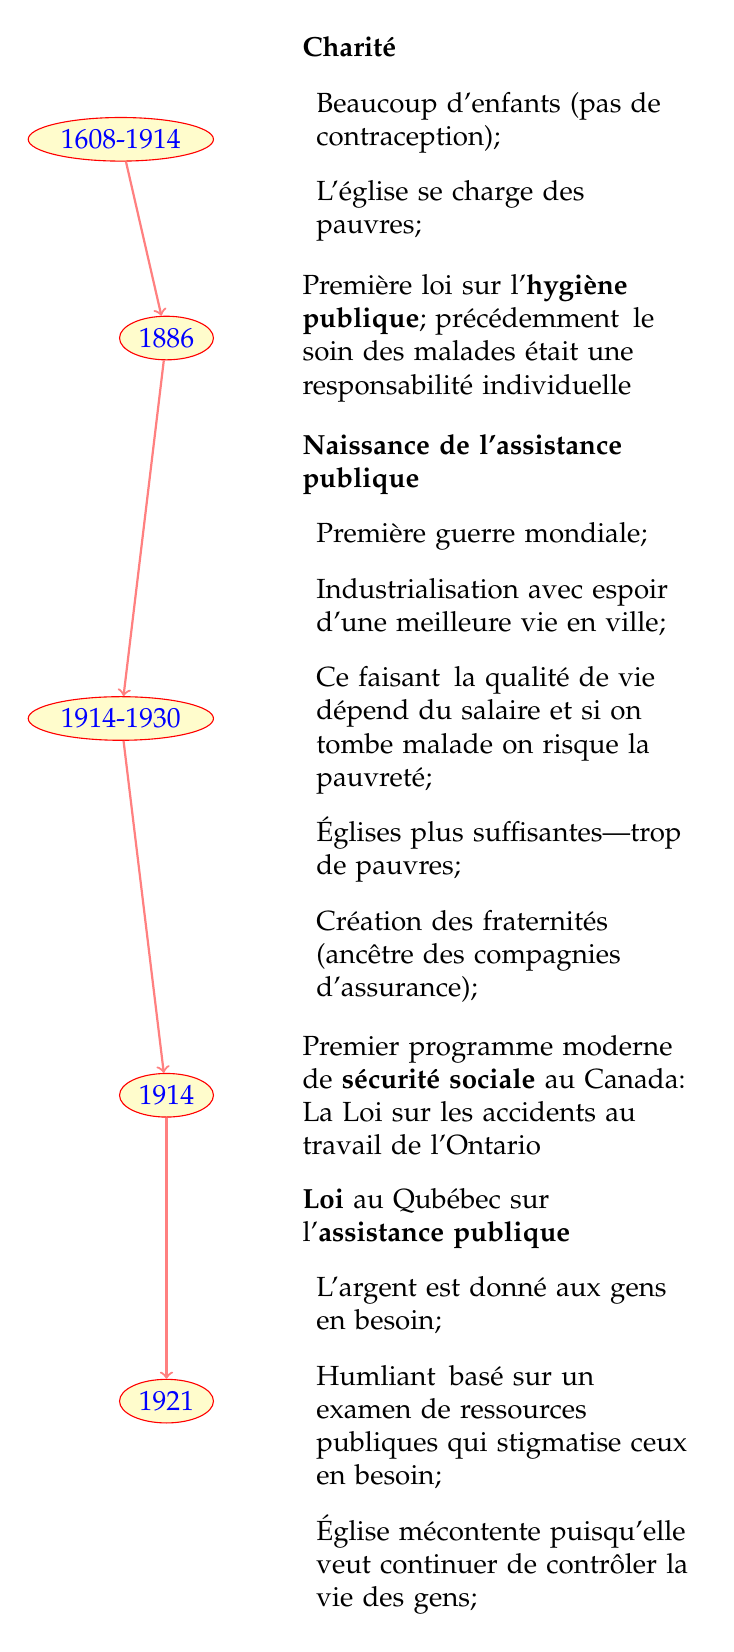
\begin{tikzpicture}[yscale = 0.5,%
           year/.style = {draw	= red,%
           				 text 	= blue,%
           				 fill 	= yellow!20,%
           				 shape 	= ellipse,%
           				 inner sep = 2pt%
           				 },%
           description/.style = {rectangle,%
           				 		align		= left,%
           				 		text width	= 50mm,%
           				 		anchor		= west%
           				 		},%
           timeline/.style = {->,%
           				 	 thick,%
           				 	 red!50%
           				 	 }%
           			]
    \foreach \year/\desc [count=\y] in {%
       1608-1914	/ \textbf{Charité}
       	\begin{itemize}[leftmargin = *]
      		\item	Beaucoup d'enfants (pas de contraception);
      		\item	L'église se charge des pauvres;
      	\end{itemize},%
      	1886	/	Première loi sur l'\textbf{hygiène publique}; précédemment\, le soin des malades était une responsabilité individuelle,%
       1914-1930	/	\textbf{Naissance de l'assistance publique}
       	\begin{itemize}[leftmargin = *]
	       	\item	Première guerre mondiale;
	       	\item	Industrialisation avec espoir d'une meilleure vie en ville;
	       	\item[]	Ce faisant\, la qualité de vie dépend du salaire et si on tombe malade on risque la pauvreté;
	       	\item	Églises plus suffisantes---trop de pauvres;
	       	\item	Création des fraternités (ancêtre des compagnies d'assurance);
       	\end{itemize},%
       	1914	/	Premier programme moderne de \textbf{sécurité sociale} au Canada: La Loi sur les accidents au travail de l'Ontario,%
       	1921	/	\textbf{Loi} au Qubébec sur l'\textbf{assistance publique} 
       	\begin{itemize}[leftmargin = *]
       		\item	L'argent est donné aux gens en besoin;
      	 	\item	Humliant\, basé sur un examen de ressources publiques qui stigmatise ceux en besoin;
     	  	\item	Église mécontente puisqu'elle veut continuer de contrôler la vie des gens;
       	\end{itemize}%
       } { \ifnum\y=1 \node[description](\y){\desc};
           \else\node[description,below=1ex of \z](\y){\desc};
           \fi
           \node[year](y-\y) [left=of \y] {\year};
           \ifnum\y>1\draw[timeline] (y-\z)-- (y-\y);\fi
           \global\let\z=\y% for drawing from last node
       }
\end{tikzpicture}
\begin{tikzpicture}[yscale = 0.5,%
           year/.style = {draw	= red,%
           				 text 	= blue,%
           				 fill 	= yellow!20,%
           				 shape 	= ellipse,%
           				 inner sep = 2pt%
           				 },%
           description/.style = {rectangle,%
           				 		align		= left,%
           				 		text width	= 50mm,%
           				 		anchor		= west%
           				 		},%
           timeline/.style = {->,%
           				 	 thick,%
           				 	 red!50%
           				 	 }%
           			]
    \foreach \year/\desc [count=\y] in {%
       1930-1940		/	\textbf{Premières étapes d'une politique sociale}%
       	\begin{itemize}[leftmargin = *]
	       	\item	\textbf{Crise} de 1929---chômage en forte hausse;
	       	\item	Accroissement des interventions gouvernementales --- le gouvernement est encore timide car il doit avoir le soutien de l'Église;
       	\end{itemize},%
       	1927	/	\textbf{Assurance vieillesse} (\textbf{\textcolor{bulgarianrose}{fédéral}}); programme très strict,%
       	1935	/	\textbf{Hôpitaux provinciaux} au lieu de municipaux; cependant\, encore trop cher pour la majorité de la population,
		1940-1960	/\textbf{Prépondérance \textcolor{bulgarianrose}{fédéral}e}: 
		\begin{itemize}[leftmargin = *]
		  \item	Les besoins engendrés par la guerre règle le problème de chômage;
			\item	Dynamisme du gouvernement \textcolor{bulgarianrose}{fédéral};
			\item	L'idée de donner à \textit{tous} un certain niveau de vie\, et non juste ceux en besoin\, pousse de l'assistance sociale à la sécurité sociale;
		\end{itemize},%
			1940	/	 \textbf{assurance chômage} (\textcolor{bulgarianrose}{fédéral}) Premier programme national,%
			1949	/	 \textbf{allocations familiales} (\textcolor{bulgarianrose}{fédérales}),%
			1952	/	 \textbf{pensions} de \textbf{vieillesse} (\textcolor{bulgarianrose}{fédérales}) non liée à la démonstration du manque de ressources%
       } { \ifnum\y=1 \node[description](\y){\desc};
           \else\node[description,below=1ex of \z](\y){\desc};
           \fi
           \node[year](y-\y) [left=of \y] {\year};
           \ifnum\y>1\draw[timeline] (y-\z)-- (y-\y);\fi
           \global\let\z=\y% for drawing from last node
       }
\end{tikzpicture}

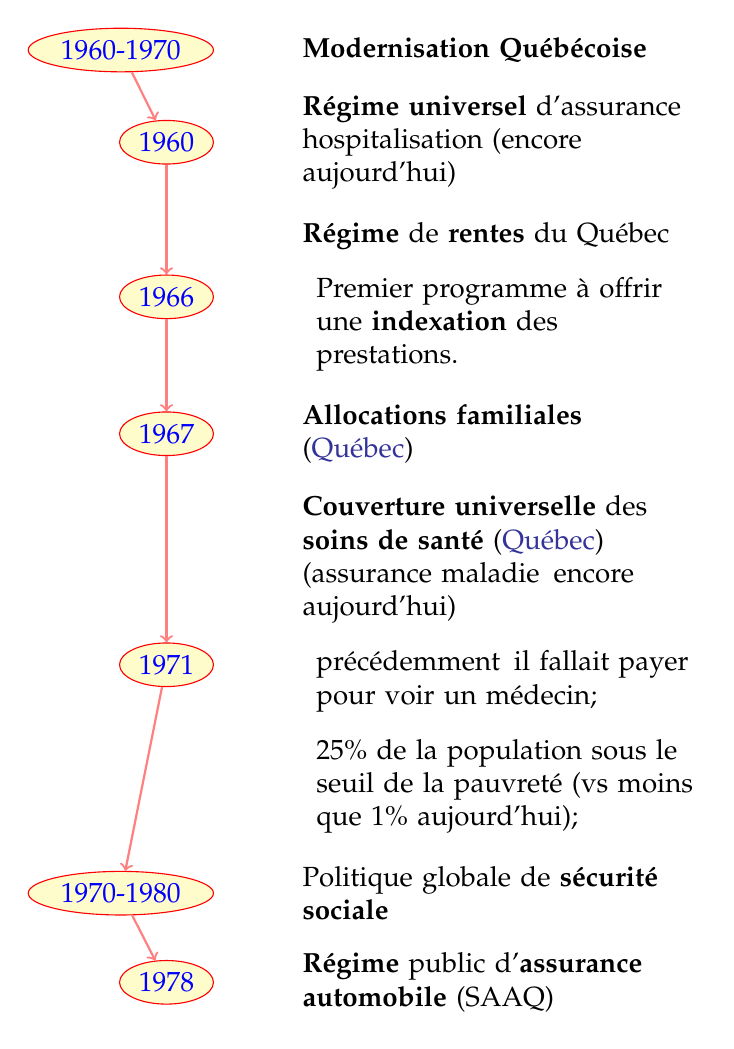
\begin{tikzpicture}[yscale = 0.5,%
           year/.style = {draw	= red,%
           				 text 	= blue,%
           				 fill 	= yellow!20,%
           				 shape 	= ellipse,%
           				 inner sep = 2pt%
           				 },%
           description/.style = {rectangle,%
           				 		align		= left,%
           				 		text width	= 50mm,%
           				 		anchor		= west%
           				 		},%
           timeline/.style = {->,%
           				 	 thick,%
           				 	 red!50%
           				 	 }%
           			]
    \foreach \year/\desc [count=\y] in {%
       	1960-1970	/	\textbf{Modernisation Québécoise},%
			1960		/	\textbf{Régime universel} d'assurance hospitalisation (encore aujourd'hui),%
			1966		/	\textbf{Régime} de \textbf{rentes} du Québec
				\begin{itemize}[leftmargin = *]
				\item	Premier programme à offrir une \textbf{indexation} des prestations.
				\end{itemize},%
			1967	/	 \textbf{Allocations familiales} (\textcolor{blue(pigment)}{Québec}),%
			1971	/	 \textbf{Couverture} \textbf{universelle} des \textbf{soins de santé} (\textcolor{blue(pigment)}{Québec}) (assurance maladie\, encore aujourd'hui)
				\begin{itemize}[leftmargin = *]
				\item	précédemment\, il fallait payer pour voir un médecin;
				\item	25\% de la population sous le seuil de la pauvreté (vs moins que 1\% aujourd'hui);
				\end{itemize},%
       	1970-1980	/	Politique globale de \textbf{sécurité sociale},%
			1978	/	\textbf{Régime} public d'\textbf{assurance automobile} (SAAQ)%
       } { \ifnum\y=1 \node[description](\y){\desc};
           \else\node[description,below=1ex of \z](\y){\desc};
           \fi
           \node[year](y-\y) [left=of \y] {\year};
           \ifnum\y>1\draw[timeline] (y-\z)-- (y-\y);\fi
           \global\let\z=\y% for drawing from last node
       }
\end{tikzpicture}

\textbf{Suite : Recul de la protection Sociale}
\begin{itemize}
	\item	Poussée inflationniste, récession \textbf{(1981-1983)}, taux de chômage élevé;
	\item	Hausse des déficits et baisse des revenus fiscaux, crise de l'endettement public;
	\item	Recul de la protection sociale avec des programmes jugés extravagants;
	\item	Politiques de restriction budgétaire;
	\item	Explosion des coûts de l'assurance maladie
		\begin{itemize}
		\item[1984: ]	Loi canadienne sur la santé---pour préserver l'universalité des soins de santé;
		\end{itemize}
	\item	Coûts d'aucun \og bon sens \fg{} avec un régime qui \textbf{va} devoir changer;
		\begin{itemize}
		\item[1997:]	Assurance médicaments (\textcolor{blue(pigment)}{Québec});
		\item[2006:]	Création d'assurance parentale (\textcolor{blue(pigment)}{Québec});
		\end{itemize}
\end{itemize}

%%%%%%

\begin{conceptgen}{Programmes sociaux au Québec / Canada}
Les 9 fonctions de l'OIT sont couvert par ces programmes:
\begin{itemize}
	\item	Assurance sociale;
	\item	Assurance emploi;
	\item	Allocations familiales;
	\item	Indemnisation accidents travail (CEESST);
	\item	Régime de Rentes du Québec (RRQ);
	\item	Régime de Pension du Canada (RPC);
	\item	Pension sécurité vieillesse (\textcolor{bulgarianrose}{fédéral}) \textbf{\textit{ET}}\\ supplément de revenu garanti (\textcolor{bulgarianrose}{fédéral})\textbf{\textit{ET}}\\ allocation au conjoint ;
	\item	Régime de santé (maladie \textbf{\textit{ET}} hospitalisation---conjoint Canada-Québec);
	\item	\textcolor{amaranth}{Assurance Automobile (\textcolor{blue(pigment)}{Québec}) (SAAQ) (Couvert dans le cours \textit{Introduction à l'actuariat I})} ;
	\item	Assurance parentale (\textcolor{blue(pigment)}{Québec});
	\item	Assurance médicaments (\textcolor{blue(pigment)}{Québec})
\end{itemize}
\end{conceptgen}

Catégories de programmes

\begin{tabularx}{\columnwidth}{| >{\columncolor{airforceblue!80}}>{\setlength\hsize{.25cm}} l | >{\columncolor{beaublue}}X  | >{\columncolor{beaublue}}X	|  >{\columncolor{beaublue}}X  |}
\hline\rowcolor{airforceblue} 
\textcolor{white}{\textbf{Programme}}	&	\textcolor{white}{\textbf{Assistance sociale}}	&	\textcolor{white}{\textbf{Assurance sociale}}		&	\textcolor{white}{\textbf{Régimes universels}}	\\\specialrule{0.1em}{0em}{0em} 
Objectif	&	protection minimale (dernier recourt)	&	protection de base			\\\hline
\end{tabularx}

\textbf{Assistance sociale}

\begin{itemize}[leftmargin = *]
	\item	\textbf{Caractéristiques}:
	\item[]	Test de résidence;
	\item[]	Test de besoin;
	\item[]	Financement gouvernementale (\textcolor{darkgreen}{pay-as-you-go});
	\item	\textbf{Aide Sociale} au \textcolor{blue(pigment)}{Québec}:
	  \item[] Prestations non-imposable;
	  \item[] 3 programmes pour ceux dans le besoin :
		  \begin{enumerate}
		  \item	Programme d'\textbf{assistance sociale} (qui s'appelait le bien-être social);
		  \item	Prime au travail;
			  \begin{itemize}
			  \item	crédit d'impôt qui vise à encourager les individus à faible revenu à rester sur le marché du travail en bonifiant leur offrant un certain soutien financier;
			  \end{itemize}
			 \item	\textbf{Supplément de revenu garanti} (\textit{SRG}) et \textbf{allocation au conjoint} (\textcolor{bulgarianrose}{fédéral});
		  \end{enumerate}
\end{itemize}


\textbf{Assurance sociale}
\begin{itemize}[leftmargin = *]
	\item	\textbf{Caractéristiques}:
	  \item[]	Contributions obligatoires;
	  \item[]	Les prestations sont en fonction de la participation (reliés aux gains);
	  \item[]	Supervision gouvernementale;
	  \item[]	Capitalisation : totale ou partielle;
		  \begin{itemize}
		  \item	L'idée de la capitalisation est que c'est de l'argent mis de côté et pas inclus dans les revenus puisqu'elle sera éventuellement dépensée comme revenu.
		  \end{itemize}
	\item Similitudes avec l'assurance privée:
	  \begin{itemize}
		  \item	Mise en commun des risques
		  \item Description des prestations
		  \item Calcul mathématique des prestations
		  \item Contributions pour financer le coût
		  \item Pas de test de besoins
		  \item Contribue à la sécurité économique
		\end{itemize}
%%%	-----
%%%	NOTES (AJVR):
%%%	+	Développer sur contributions? 
%%%	+	Donner des exemples de programmes obligatoires;
%%%	+	Les prestations ça m'est un peu flou live j'ai moyen compris la façon qu'elle l'a dit mais j'en n'ai pas saise une assez bonne compréhension pour bien l'expliquer, toi?
%%% + va falloir aller lui demander ! Je me fais une liste de questions 
%%%	-----
\begin{center}
\begin{tabular}{| >{\columncolor{beaublue}}c | >{\columncolor{beaublue}}c  |}
\hline\rowcolor{airforceblue} 
\textcolor{white}{\textbf{Avantages}}	&	\textcolor{white}{\textbf{Désavantages}}		\\\specialrule{0.1em}{0em}{0em} 
Protection de base	&	non-universel	\\\hline
Redistribution de l'argent	&	insuffisant	\\\hline
\end{tabular}
\end{center}
%%%	-----
%%%	Comment trouves-tu ce format pour les commentaires? Je trouve ça pourrait être idéal!
%%%	NOTES (AJVR):
%%%	+	Reste à développer sur ceci, voudrait peut-être la peine de ne pas le mettre en forme de tableau mais je me pratiquais;
%%%	+	Ajouter similitude avec assurance privée?
%%% + J'aime ca ! Je vois pas quoi ajouter d'Autres et meme le tableau est clean je trouves ca ok. 
%%%	-----
\end{itemize}
%%%	-----
%%%	Breakdown de tableaux (AJVR):
%%%	Les tableaux c'est compliqué en LaTeX, je t'explique divers composantes ici:
%%%	+	Le premier argument après "begin{tabular}" est l'alignement des colonnes;
%%%	+	"c" pour center, "l" pour left-aligned, "r" pour right-aligned;
%%%	+	les barres "|" ajoute une barre verticale entre colonnes;
%%%	+	on met autant de lettre d'alignement que de colonnes désirées;
%%%	+	"tabular" est l'environnement pour créer les tables;
%%%	+	"airforceblue" est une des couleurs que j'ai défini dans le préambule, airforceblue!80 implique que j'y donne une opacité de 80%;
%%%	+	\columncolor va ensuite appliquer cette couleur à la _colonne_ en entier;
%%%	+	il est entouré de >{} pour y dire d'appliquer cette couleur à la position d'alignement "c"
%%%	+	en revanche, \rowcolor applique une couleur à une _rangée_ en entière;
%%%	+	\hline crée une _ligne_ _h_orizontale;
%%%	+	On sépare les items de la table avec "&" et fini la ligne avec "\\";
%%%	+	\shortstack crée comme une "boite" de texte ce qui fait que je peux créer plusieurs lignes;
%%%	+	Ceci sert uniquement à avoir plusieurs lignes de texte dans une même cellule;
%%%	+	\shortstack[l] est pour y indiquer d'aligner le texte à la gauche.
%%%	-----
\begin{center}
	\textbf{Comparaison d'assurance sociale et privée}
\begin{tabular}{| >{\columncolor{airforceblue!80}}l | >{\columncolor{beaublue}}l  | >{\columncolor{beaublue}}l |}
\hline\rowcolor{airforceblue} 
\textcolor{white}{\textbf{Assurance}}		&	\textcolor{white}{\textbf{Sociale}}		&	\textcolor{white}{\textbf{Privée}}		\\\specialrule{0.1em}{0em}{0em} 
Participation	&	obligatoire	&	facultative		\\\hline
Équité			&	sociale		&	individuelle		\\\hline
Base				&	légale		&	contractuelle	\\\hline
Contexte			&	monopole		&	compétition		\\\hline
\shortstack[l]{Facilité de \\ prévision des\\ coûts}	&	difficile 	&	\shortstack[l]{facile (tout\\ le monde\\ est couvert)}		\\\hline
Capitalisation	&	pas toujours	&	pleinement		\\\hline
\shortstack[l]{Sélection\\ des risques}	&	\shortstack[l]{aucune (peut pas \\ décider d'exclure\\ une personne)}	&	\\\hline
Indexation	&	au coût de la vie	&	rarement		\\\hline
But		&	sécurité sociale	&	\shortstack{couvrir ceux\\ qui le désirent}	\\\hline
\end{tabular}
\end{center}
Donc il y a des similitudes mais leur objectif diffère de façon significative.





\textbf{Régimes universels}
\begin{itemize}[leftmargin = *]
	\item	\textbf{Caractéristiques}:
	  \item[]	Obligatoire et universel;
	  \item[]	Pas de tests de besoins;
	  \item[]	Éligibilité basée sur la résidence (Citoyenneté);
	  \item[]	Prestations fixes définies par la loi;
	  \item[]	Pas de Capitalisation (financés par les recette du gouvernement);
%%%	-----
%%%	NOTES: (AJVR)
%%%	+	J'étais tanné et je n'ai vraiment pas mis beaucoup de détails rendu ici;
%%%	+	Ajouter
%%%	-----
\begin{center}
\begin{tabular}{| >{\columncolor{beaublue}}c | >{\columncolor{beaublue}}c  |}
\hline\rowcolor{airforceblue} 
\textcolor{white}{\textbf{Avantages}}	&	\textcolor{white}{\textbf{Désavantages}}		\\\specialrule{0.1em}{0em}{0em} 
Simple	&	Pas relié aux besoins	\\\hline
Combat la pauvreté	&	Coût caché	\\\hline
	&	Faibles prestations	\\\hline
\end{tabular}
\end{center}
\end{itemize}

Classement des régimes existants

\begin{tabular}{| >{\columncolor{beaublue}}m{2cm} | >{\columncolor{beaublue}}m{2.5cm} | >{\columncolor{beaublue}}m{2.5cm} |}
\hline\hline\rowcolor{airforceblue} 
\textcolor{white}{\textbf{Assurance emploi}}						&	\textcolor{white}{\textbf{Assistance sociale}}	&	\textcolor{white}{\textbf{Régimes universels}}	\\\hline
Assurance parentale					&	Assistance sociale						&	Allocations familiales	\\
\hline
Régime de rentes du Québec (R.R.Q.)	&	Prime au travail				&	soins de santé	\\
\hline
Santé Sécurité	au Travail (SST)		&	Supplément de revenu garanti	&	Sécurité de la vieillesse	\\
\hline
Assurance automobile					&	Allocation au conjoint					&	\\
\hline
Assurance médicament					&											&	\\\hline
\end{tabular}

\textbf{Régimes sociaux sous tension}
\begin{itemize}[leftmargin = *]
	\item	Vieillissement de la population;
	\item Changements démographiques (Les \textit{Boomers} sont beaucoup !);
	\item Complexité administrative
	\item Évolution de la société depuis leur mise en place;
	  \begin{itemize}
	  \item Par exemple, la \textit{rente du Survivant}. Le salaire ne vient plus seulement du mari, à revoir ? 
	  \end{itemize}
	\item Répartition de la richesse
	\item Abus
	\item La mondialisation mène à la compétition
	  \begin{itemize}
	  \item Maintenant qu'on sait ce que les autres pays font, on sait ce qui se fait mieux, on veut compétitionner
	  \end{itemize}
\end{itemize}
Nos régimes craquent d'un peu partout. On mets en vigueur des changements et des lois pour cacher ces fissures, mais ça va sans doute exploser un jour.\\

\textbf{Les États-Unis}

\begin{itemize}[leftmargin = *]
	\item	Les droits sociaux ne sont pas dans la constitution;
	\item Vision différente:
	  \begin{itemize}
	  \item Selon eux, la meilleure assistance sociale reste le plein emploi : ils cherchent à maintenir la croissance économique et à faire baissser le chômage.
	  \end{itemize}
	\item Protection des démunis : axée sur l'aide sociale plutôt que la sécurité;
	  \begin{itemize}
	  \item On s'occupe des pauvres après (mesure humiliante : \textit{food ticket} pour l'épicerie)
	  \item 6 volets à la sécurité sociale:
	  \begin{enumerate}
	    \item Vieillesse et décès (survivants) (\textcolor{bulgarianrose}{fédéral})
	    \item Invalidité (\textcolor{bulgarianrose}{fédéral})
	    \item Médicare (Medicaid) (\textcolor{bulgarianrose}{fédéral})
	    \item Chômages (États)
	    \item Accidents de travail et maladies professionnelles (États)
	    \item Assurance maladie (Obama Care)
	  \end{enumerate}
	\item Obama Care (détails) : 
	  \begin{itemize}
	    \item Obligation aux individus de souscrire si non-couvert par leur employeur
	    \item Interdiction de refuser de couvrir un individu en raison d'antécédents médicaux (du côté des assureurs)
	    \item le gouvernement accorde de l'aide pour payer la prime si le revenu est entre 1 à 4 fois le seuil de la pauvreté
	    \item \textbf{supprimé le 1er Janvier 2019 }
	    \item Certains états ont maintenu l'obligation de détenir de l'assurance maladie
	    \item[] Exemple : \textit{Massachussett}, \textit{New Jersey} et \textit{Columbia}
	 \end{itemize}
	 \end{itemize}
	 \end{itemize}
 Les raisons d'un tel régime était qu'au \textit{États-Unis}, 64\% des faillites étaient liées aux frais de santé
\newpage

\section{Le système de retraite au Canada}

\begin{definitionNOHFILL}[Vie active]
Période de vie où 
\begin{itemize}[leftmargin = *]
	\item	On est \textbf{actif} sur le \textbf{marché du travail};
	\item	Les \textbf{revenus} proviennent principalement de revenus \textbf{d'emploi}.
\end{itemize}
\end{definitionNOHFILL}

\begin{definitionNOHFILL}[La retraite]
Période de la vie où l'on est, ou considéré comme étant, \textbf{incapable de travailler}. Il s'ensuit que le revenus ne provient pas d'emploi.

\begin{conceptgen}{Objectifs de la protection}
\begin{itemize}[leftmargin = *]
	\item	Compenser la \textbf{perte de revenu} associée à la retraite;
	\item	Contrer la pauvreté des personnes âgées;
	\item	Maintenir en emploi ou favoriser le retrait des travailleurs âgés (Incitatif).
\end{itemize}
\end{conceptgen} 

\begin{conceptgen}{\textbf{Types de revenus} à la retraite}
\begin{itemize}[leftmargin = *]
	\item	Rentes de l'état: gouvernement paye des rentes (régime public, souvent insuffisant);
	\item[] RRQ, PSV;
	\item	Rentes de l'employeur: certains employeurs payent des rentes (régime privé);
	\item	Épargne personnelle (patrimoine): la proportion du revenu dépend de l'épargne de l'individu;
	\item	Aide sociale pour personnes âgées;
	\item[] SRG pour les plus démunis.
\end{itemize}
\end{conceptgen} 
\end{definitionNOHFILL}

%%%

\begin{definitionNOHFILL}[Âge normal de retraite (ANR)]
Âge de début de retraite utilisée pour le calcul des prestations payables à la retraite. Cet âge est loin de l'âge effectif de la retraite actuel, il s'agit simplement de l'âge théorique utilisé pour les calculs.

\begin{rappel_enhanced}[Historique]
\begin{itemize}[leftmargin = *]
	\item	L'ANR est de 65 ans depuis 1970 (Harper avait décidé d'augmenter cet âge graduellement entre 2023 et 2029, Trudeau est venu contre cette décision);
	\item	Dans le passé, l'ANR était de 65 ans pour les hommes et 60 ans pour les femmes---cette pratique maintenant considérée discriminatoire et interdite;
	\item	Les régimes publics l'utilisent et c'est l'âge maximal permis pour les régimes privés;
	\item	Ce n'est pas un âge obligatoire pour les contribuables.
\end{itemize}
\end{rappel_enhanced}

\begin{conceptgen}{Retraite anticipée}
\begin{itemize}[leftmargin = *]
	\item	Prendre sa retraite plus tôt implique une \textbf{réduction actuarielle};
	\item	La loi peut prévoir qu'une rente sans réduction peut être versée à \textit{certaines conditions};
		\begin{itemize}[leftmargin = *]
		\item	Par exemple, selon le \textbf{nombre d'années de service}, comme dans l'armée, une pension complète peut-être payée après seulement 25 ans.
		\end{itemize}
	\item	\textcolor{red}{Ce sujet est vu plus en profondeur dans les cours de Régimes de retraites.}
\end{itemize}
\end{conceptgen} 
\end{definitionNOHFILL}

\begin{rappel_enhanced}[Historique de la retraite]
Historiquement, la retraite était rare et courte. Avec l'augmentation de l'espérance de vie est venu des changements majeurs au niveaux de la durée de la retraite. 

Ce tableau illustre assez bien l'historique de la retraite:

\centerline{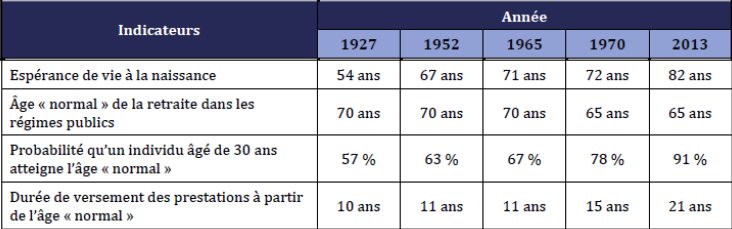
\includegraphics[scale=0.32]{src/ACT-1005/retraite-age-hist.png}}

\begin{itemize}[leftmargin = *]
		\item	La vie active a donc diminué avec la \textbf{diminution de l'ANR} et la \textbf{retraite anticipé};
		\item	La durée de la retraite est passée de 10 à 21 ans, menant à de grandes \textbf{pressions financières} sur le système de retraite;
		\item	De plus, le coût de la vie a augmenté et cette \textbf{inflation} \textit{multiplie les pressions} sur les \textbf{longues périodes de paiements} (20 ans et plus).
\end{itemize}
\end{rappel_enhanced}

%%%

\begin{rappel_enhanced}[Baby Boom]
\begin{itemize}[leftmargin = *]
	\item	Génération d'enfants nés après la fin de la Deuxième Guerre mondiale (taux de natalité élevé);
	\item[]	Nés dans les alentours \textit{approximatifs} de 1946 à 1965.
	\item	Le nombre moyen d'enfants par femme était de 3.7 (4.1 dans les années 50);
	\item[]	En contraste, c'est de 1.6 enfants par femme aujourd'hui.
	\item	Le départ des baby-boomers à la retraite a un impact socio-économique important.
	\item[] principalement car les hauts taux de natalité ne seront pas renouvelés.
\end{itemize}
\end{rappel_enhanced}

\begin{rappel_enhanced}[Baby Bust (génération X)]
\begin{itemize}[leftmargin = *]
	\item	Enfants nés dans les alentours \textit{approximatifs} de 1966 à 1976.
	\item	Génération coincée entre les baby-boomers et la génération Y;
	\item	Difficulté à trouver des emplois en raison du grand nombre de baby-boomers.
\end{itemize}
\end{rappel_enhanced}

\begin{conceptgen}{Proportion de la population active}
Les graphiques de pyramides d'âges permettent la visualisation de l'augmentation importante de la population âgée. L'\textbf{insuffisance} de la \textbf{population active} pour \textbf{soutenir} le \textbf{régime de retraite} actuel s'ensuit.

En \textbf{contraste} aux \textbf{États-Unis} (1.9\%) et le \textbf{reste du Canada} (5.1\%), la \textbf{population active du \textcolor{blue(pigment)}{Québec}} entre 20 et 64 ans va \textbf{diminuer} (-3.6\%) de 2015 à 2030. 
\end{conceptgen} 

\begin{itemize}[leftmargin = *]
	\item	Enfants nés dans les alentours \textit{approximatifs} de 1966 à 1976.
	\item	Génération coincée entre les baby-boomers et la génération Y;
	\item	Difficulté à trouver des emplois en raison du grand nombre de baby-boomers.
\end{itemize}
%%%

\begin{conceptgen}{Approches des régimes de retraite}
\textbf{Beveridge}
\begin{itemize}[leftmargin = *]
	\item	Approche d'une rente \textbf{universelle};
	\item	Verse à tous les individus une rente;
	\item	Prestations aux démunis.
\end{itemize}
\tcbline
\textbf{Bismark}
\begin{itemize}[leftmargin = *]
	\item	Approche d'une rente pour les \textbf{travailleurs}.
\end{itemize}
\end{conceptgen}

\begin{conceptgen}{Adhésion à un régime de revenu à la retraite}
Les régimes peuvent être \textbf{obligatoires} ou \textbf{volontaires}.

\textbf{Obligatoire}
\begin{itemize}[leftmargin = *]
	\item	Tous les individus doivent cotiser pour leurs retraites;
	\item	Garanti que tout le monde se constitue une retraite.
\end{itemize}

\textbf{Volontaire}
\begin{itemize}[leftmargin = *]
	\item	Les gens ont tendance à sous-estimer leurs besoins futurs et ne pas épargner suffisamment d'argent;
	\item	La présence d'un système obligatoire n'empêche pas celle d'une épargne supplémentaire par un régime facultatif;
\end{itemize}

\begin{center}
	\textbf{Exemples}
\end{center}

\textbf{État}
\begin{itemize}[leftmargin = *]
	\item	Pension de la sécurité de vieillesse (PSV) \textcolor{brickred}{(obligatoire)};
	\item	Régie des rentes du Québec (RRQ) \textcolor{brickred}{(obligatoire)}.
	\item	Régime de Pension du Canada (RPC) \textcolor{brickred}{(obligatoire)}.
\end{itemize}
\textbf{Privé}
\begin{itemize}[leftmargin = *]
	\item	Régimes complémentaires de retraite (RCR) \textcolor{brickred}{(habituellement obligatoire s'il est présent)};
	\item	Régime \textbf{volontaire} d'épargne-retraite (RVER) \textcolor{blue}{(facultatif)};
	\item	Régime enregistré d'épargne-retraite (REER) \textit{collectif} \textcolor{blue}{(facultatif)}.
\end{itemize}
\textbf{Individuel} \textcolor{blue}{(facultatifs)}
\begin{itemize}[leftmargin = *]
	\item	Compte d'épargne libre d'impôt (CELI), REER, épargne, biens (maisons, \dots).
\end{itemize}
\end{conceptgen}

\begin{conceptgen}{Financement}
\begin{center}
\textbf{Capitalisation} (\textbf{funded})
\end{center}

\textbf{Procédure}
\begin{enumerate}[leftmargin = *]
	\item	Participants actifs versent leurs cotisations;
	\item	Le régime place les sommes au nom de chaque participant;
	\item	Au moment de la retraite, ces mêmes montants lui sont restitués sous forme de rente.
\end{enumerate}

\textbf{Détails}
\begin{itemize}[leftmargin = *]
	\item	Il est possible d'avoir une capitalisation totale ou partielle;
	\item	Les sommes sont considérables et servent de financement pour les gouvernements et industries;
	\item	Fonctionnement se rapproche à celui d'une compagnie d'assurance.
\end{itemize}

\textbf{Risques}
\begin{itemize}[leftmargin = *]
	\item	\textbf{Fluctuations} de l'économie;
	\item	\textbf{Faillites} d'entreprises;
	\item	\textbf{Corruption} (malversations).
\end{itemize}

\tcbline

\begin{center}
\textbf{Répartition} (\textcolor{darkgreen}{Pay-as-you-go (PAYG)})
\end{center}

\textbf{Procédure}:
\begin{enumerate}[leftmargin = *]
	\item	Participants actifs versent leurs cotisations;
	\item	Le régime utilise les sommes pour payer les pensions des retraités actuels.
\end{enumerate}

\textbf{Détails}
\begin{itemize}[leftmargin = *]
	\item	Repose sur une forte solidarité entre générations;
	\item	Sa viabilité dépend du rapport entre le nombre de cotisants et le nombre de personnes retraitées;
	\item	Aucun actif mis de côté;
	\item	Dois presque forcément être un régime obligatoire et public.
\end{itemize}

\textbf{Risques}
\begin{itemize}[leftmargin = *]
	\item	Dépend de la \textbf{croissance de la masse salariale} puisque les cotisations sont prélevés sur les payes;
\end{itemize}
\end{conceptgen}

\begin{conceptgen}{Paliers du système équilibré canadien de la retraite}
\centerline{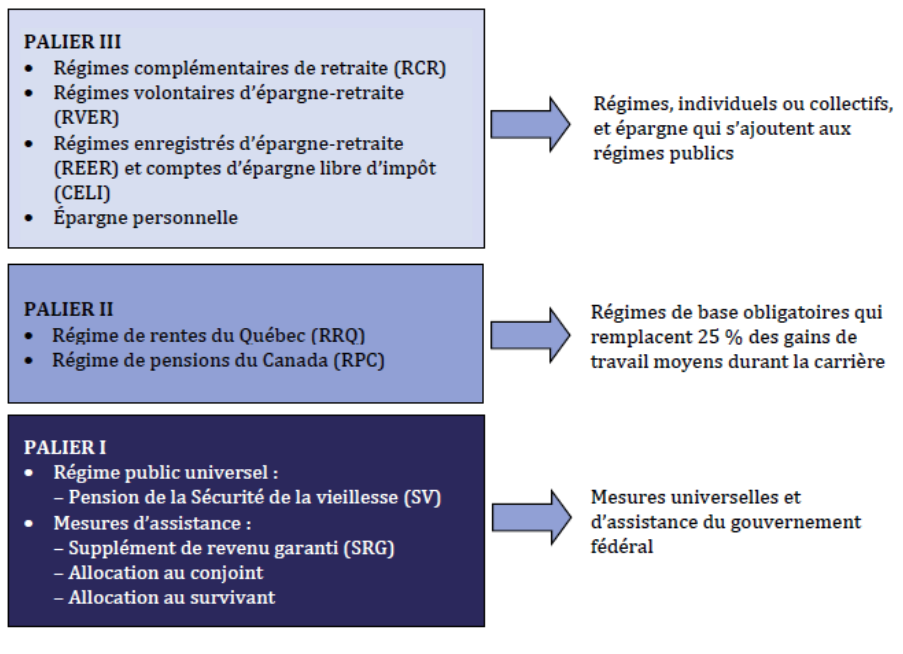
\includegraphics[scale=0.25]{src/ACT-1005/retraite-paliers.png}}

\textbf{Palier I et II}
\begin{enumerate}[leftmargin = *]
	\item	Composante \textbf{publique};
	\item	But d'\textbf{éliminer} au maximum la \textbf{pauvreté} des personnes âgées;
	\item	\textbf{Répartit les revenus} des gens tout au long de leur vie pour assurer un certain niveau de remplacement de revenu.
\end{enumerate}

\textbf{Palier III}
\begin{enumerate}[leftmargin = *]
	\item	Composante \textbf{privée}.
\end{enumerate}
\end{conceptgen}

\begin{conceptgen}{Remplacement de revenu à la retraite}
\paragraph{Principe de base}Règle générale qu'on doit compter sur un remplacement de 70\% de son revenu avant la retraite afin de maintenir le \textbf{même} niveau de vie. Cela ne tient pas compte cependant du \textbf{niveau de revenu} ni du \textbf{type de retraite} visé.
\\

Raisons pourquoi pas 100\%:
\begin{itemize}[leftmargin = *]
	\item	Dépenses transport moindre;
	\item	Fin de dépenses hypothécaires;
	\item	Départ d'enfants (études, nourriture, \dots);
	\item	Dépenses générales moindres (rabais, \dots);
	\item	Fin des charges sociales (parents à charge);
	\item	Fin de l'épargne retraite.
\end{itemize}
\tcbline
\textbf{Provenance} de revenu à la retraite
\begin{itemize}[leftmargin = *]
	\item	L'objectif des régimes gouvernementaux est de remplacer $Y\%$ pour les personnes gagnant un certain salaire;
	\item	Ce salaire, appelé le \textbf{maximum des gains admissibles} (\textit{MGA}), est déterminé annuellement par la \textit{RRQ};
	\item	L'importance de chaque palier va donc varier entre individus selon leur revenu.
	\item[] Plus les revenus de travail moyens sont faibles avant le retrait du marché du travail, plus les régimes publics jouent un rôle important (les gens à faibles revenus n'aurons pas assez d'argent pour en mettre de côté) 
\end{itemize}
\end{conceptgen}

\newpage

\section{Loi sur la sécurité de la vieillesse}
\begin{conceptgen}{Types de prestations}
Il existe plusieurs types de prestations dont:
\begin{itemize}[leftmargin =  *]
	\item	\hyperref[sec:PSV]{Pension de la sécurité de la vieillesse (\textit{PSV})};
	\item	\hyperref[sec:SRG]{Supplément du revenu garantie (\textit{SRG})};
	\item	\hyperref[sec:Alloc]{Allocation (au conjoint)};
	\item	\hyperref[sec:Alloc_survival]{Allocation (de survivant)}.
\end{itemize}
\end{conceptgen}

\begin{rappel_enhanced}[Historique]
%%%	--------------
%%%	NOTE
%%%	+	Voir cette page de "l'encyclopédie canadienne" (https://www.thecanadianencyclopedia.ca/fr/article/pension-de-vieillesse);
%%% +   Intéressant, explique bien en détail avec une meilleure idée sur les contextes de l'époque. (OC)
%%%	--------------
\begin{description}
	\item[1952]	Entrée en vigueur de la loi de la sécurité et vieillesse;
		\begin{itemize}[leftmargin = *]
		\item	Programme \textcolor{bulgarianrose}{fédéral};
		\item	Au niveau \textcolor{blue(pigment)}{provincial}, il n'y a pas encore grand-chose de développé;
		\item	Idée de \hl{garantir à \textbf{tous}} les citoyens \hl{âgés} (70 ans et plus) une \hl{pension non-liée au revenu} avec la PSV.
		\end{itemize}
	\item[1966]	Entrée en vigueur du \textit{RPC} et \textit{RRQ};
		\begin{itemize}[leftmargin = *]
		\item	Inclut une révision de la \textit{PSV}---élargir la portée, revoir le programme, etc.;
		\item	Programmes obligatoires.	
		\end{itemize}
	\item[1967]	Entrée en vigueur du \textit{SRG}
		\begin{itemize}[leftmargin = *]
		\item	Supplément au \textit{PSV} temporaire jusqu'au début des paiements du \textit{RCP} et \textit{RRQ};
		\item	Initialement supposé être temporaire pour aider ceux déjà à la retraite, car le \textit{RCP} et \textit{RRQ} n'allaient pas payer de prestations avant 10 ans;
		\item	Diminution de l'âge d'admissibilité à 65 ans;
		\item	Augmentation du montant des pensions.
		\end{itemize}
%%%	--------------
%%%	NOTE
%%%	+	Je trouves ça hyper pertinent, mais penses-tu qu'on devrait se limiter au contenu du cours ? (je penses à ceux qui paniquent pour rien en lisant du "nouveau contenu")(OC)
%%%	+	Ajout de colour code --- orange pour l'extra (AJVR)
%%%	--------------
	\item[1975]	Entrée en vigueur de l'Allocation au conjoint ;
		\begin{itemize}[leftmargin = *]
		\item	{\color{burntorange} Lorsqu'un seul membre du couple reçoit la \textit{PSV} et le \textit{SRG} et que l'autre a entre 60 et 64 ans;
		\item	Éventuellement renommé \og Allocation \fg{}.}
		\end{itemize}
	\item[1985]	Entrée en vigueur de l'allocation au conjoint veuf.
		\begin{itemize}[leftmargin = *]
		\item	{\color{burntorange} Extension à l'allocation au conjoint pour inclure les veuf(ve)s à faible revenu entre 60 et 64 ans dont le conjoint décédé était prestataire de la PSV et le SRG;
		\item	Éventuellement renommé \og allocation de survivant \fg{}.}
		\end{itemize}
\end{description}
\end{rappel_enhanced}

\subsection{Pension de sécurité à la vieillesse (\textit{PSV})}
\label{sec:PSV}
\begin{definitionNOHFILL}[Définition]
Régime \textbf{universel} assurant un revenu \textit{minimum} à la retraite tout citoyen canadien \textbf{admissible}. 
\hl{Le but est de couvrir \textit{environ} 15\% des revenus avant retraite} pour le \hl{travailleur moyen}.
\end{definitionNOHFILL}

\begin{conceptgen}{Admissibilité}
\begin{itemize}[leftmargin = *]
	\item	Sujet à un \hl{test de résidence}---doit: 
		\begin{enumerate}[leftmargin = *]
		\item	être citoyen canadien \\
					\textbf{ou}\\
				être un résident autorisé;
		\item	avoir habité au Canada pendant au moins 10 ans après l'âge de 18 ans;
		\end{enumerate}
	\item	Si quitte le Canada, doit avoir habité au Canada pendant au moins 20 ans après l'âge de 18 ans;
	\item[]	\textbf{Note}: Il y existe d'autres possibilités selon ententes avec d'autres pays (comme les É.-U.);
	\item	Pas de test de besoin, mais possibilité de devoir la rembourser (\hypertarget{recup_tx_l8r1}{\hyperlink{recup_tx_explain}{\textcolor{blue_rectangle}{impôt de récupération}}});
	\item   Aucun critère lié au travail;
	\item	Doit être d'au moins l'ANR (65 ans), mais \textit{pas besoin d'être retraité};
\end{itemize}
\end{conceptgen}

\begin{conceptgen}{Montant de la rente}
Établi selon le nombre d'années où l'individu a habité au Canada après l'âge de 18 ans.

\paragraph*{Pension complète}
\begin{itemize}[leftmargin = *]
	\item	Si 40 ans de résidence au Canada après l'âge de 18 ans;
	\item	Dont au moins 10 ans immédiatement avant la demande \\
				\textbf{ou} 	\\
			1 an de résidence avant la demande et 3 ans de résidence avant l'âge de 55 ans pour chaque année manquante du 10 ans. \textcolor{burntorange}{(S'applique pour certaines personnes ayant passés des années à l'étranger avec un pays ayant une entente. Cas précis non important)}
\end{itemize}

\paragraph*{Pension partielle}
\begin{itemize}[leftmargin = *]
	\item	Au moins 10 ans de résidence au Canada après l'âge de 18 ans;
	\item	Un quarantième (1/40) de la pension pour chaque année après 18 ans;
	\item	Une pension partielle \textbf{ne} peut \textbf{pas} être augmentée après son approbation en fonction du nombre d'années de résidence supplémentaire.
\end{itemize}
\end{conceptgen}

\begin{conceptgen}{Particularités du paiements}
\begin{description}
	\item[Étranger]	Avoir vécu au Canada pendant au moins 20 ans après l'âge de 18 ans;
		\begin{itemize}[leftmargin = *]
		\item 	Si non respectée, les paiements à l'extérieur du Canada auront lieu seulement pour le mois du départ et les 6 mois suivants.
		\item	Note que l'on peut être absent du Canada pour plus que 6 mois sans perdre son droit de cumuler. Le temps avant le départ n'est pas perdu, il est possible de continuer à cumuler à partir du retour du voyage.
		\end{itemize}
	\item[Report] En échange d'une pension plus élevée, il est possible depuis juillet 2013 de reporter la PSV jusqu'à 5 ans;
		\begin{itemize}[leftmargin = *]
		\item	Augmentation de 0.6\% pour chaque mois de report jusqu'à un maximum de 36\% à l'âge de 70 ans (modification actuarielle).
		\item   L'impôt de récupération explique pourquoi certaines personnes pourraient vouloir reporter leur PSV (\textcolor{red}{expliqué plus tard}).
		\end{itemize}
	\item[Indexation]	Le montant de la rente est indexé à l'IPC à chaque trimestre.
\end{description}
\end{conceptgen}

\begin{conceptgen}{Fiscalité}
\begin{itemize}[leftmargin = *]
	\item	La prestation est imposable (\textcolor{bulgarianrose}{fédéral} et \textcolor{blue(pigment)}{provincial});
	\item	Depuis 1989, il existe un \hypertarget{recup_tx_explain}{\hyperlink{recup_tx_l8r1}{\textcolor{blue_rectangle}{impôt de récupération}}} qui s'impose lorsque le revenu excède un certain seuil;
	\item	Le seuil de revenu maximal en 2019 était de 77 580\$ et donc la récupération serait 15\% du revenu net \textbf{en excès de} ce montant (celle-ci n'est donc pas complètement universelle);
	\item	Il est possible de récupérer la PSV en entier (dès 126 058\$);
	\item	Puisque \hl{le test de revenu est individuel} et non par couple, il est possible d'être créatif avec ses finances.
\end{itemize}
\end{conceptgen}

\begin{conceptgen}{Âge à la retraite}
	\begin{itemize}[leftmargin = *]
		\item	Le gouvernement \textit{Harper} avait annoncé en 2012 l'intention de hausser graduellement l'âge de la retraite de 65 à 67 ans (2023-2029);
				\begin{itemize}[leftmargin = *]
				\item Le but était d'assurer la préservation du programme, compte tenu de l'augmentation de l'espérance de vie à la hausse.
				\end{itemize}
		\item	Le gouvernement \textit{Trudeau} a annoncé l'annulation de l'intention de hausser de l'\textit{ANR} en 2016;
		\item	La \hl{raréfaction de la main d'oeuvre} va mettre une \hl{pression} sur les travailleurs de \hl{rester sur le marché du travail plus longtemps};
		\item	L'ICA a pris position publiquement en avril 2019 pour une augmentation de l'ANR en échange de prestations plus élevées.
				\begin{itemize}[leftmargin = *]
				\item Pour la \textit{PSV}, cela impliquerait une prestation payable à 67 ans au lieu de 65 ans.
				\item Un revenu encore plus élevé à la retraite assurerait une meilleure protection contre les coûts associés au risque de longévité.
				\end{itemize}
	\end{itemize}
\end{conceptgen}

\begin{conceptgen}{Financement}
Le financement de la \textit{PSV} est \textcolor{darkgreen}{pay-as-you-go}, il n'y a pas de caisse distincte et sort directement des impôts.
\begin{itemize}[leftmargin = *]
	\item En raison du vieillissement de la population, le coût du programme augmente à un taux très supérieur à la croissance du \textit{PIB}.
\end{itemize}
\end{conceptgen}

\columnbreak

\subsection{Supplément de revenu garanti (\textit{SRG})}
\label{sec:SRG}
\begin{definitionNOHFILL}[Définition]
Prestation mensuelle non imposable offerte aux bénéficiaires de la \textit{PSV} ayant un faible revenu résidant au Canada. (Rappel : depuis 1967)
\end{definitionNOHFILL}

\begin{conceptgen}{Admissibilité}
\begin{itemize}[leftmargin = *]
	\item	Recevoir la \textit{PSV}---le \textit{SRG} peut être reçu à partir du même mois que la \textit{PSV};
	\item	Avoir des gains faibles---prestation réduite selon les autres revenus de la personne ou du conjoint;
	\item	Présenter une nouvelle demande annuellement.
\end{itemize}
\end{conceptgen}

\begin{conceptgen}{Montant de la prestation}
Établi en fonction de l'état conjugal et du revenu de l'année précédente.\\

La définition de revenus:
\begin{description}
	\item[exclus]	la \textit{PSV} et l'allocation;
	\item[inclus]	\textit{RRQ}, \textit{REER}, \textit{RCR}, placements, loyers, gains en capitaux, emplois, etc.
\end{description}

\textbf{Montants maximaux} mensuels (\textit{1$^{\text{er}}$ Janvier 2020}):
\begin{itemize}[leftmargin = *]
	\item	Personne seule ou personne ayant un conjoint qui ne \textit{reçoit pas la PSV} : 916.38\$;
	\item	Personne ayant un conjoint qui \textit{reçoit la PSV ou l'Allocation} : 551.63\$;
\end{itemize}

\textbf{Caractéristiques} : 
\begin{itemize}[leftmargin = *]
	\item	Depuis 2008, il est possible d'avoir jusqu'à 3 500\$ de revenus d'emploi sans impact sur la prestation---ce montant \textit{devrait} augmenter à 5 000 \$ en 2020 avec une pénalité de seulement 50\% pour les 10 000\$ suivants;
	\item	Réduction de 1\$ pour chaque 2\$ de revenu autre (1\$ par rentes pour chaque 4\$ de gains combinés dans le cas d'un couple tous deux prestataires);
	\item	Le montant est déterminé annuellement selon les gains de l'année précédente et donc il peut fluctuer dans le temps.
\end{itemize}
\end{conceptgen}

\begin{conceptgen}{Particularités du paiement}
\begin{description}
	\item[Demandes]	Les prestataires doivent faire leur demande annuellement;
	\item[Étranger]	Aucune prestation pour le non-résident du Canada (les prestations cessent si le pensionné quitte le Canada pendant plus de 6 mois);
	\item[Indexation]	Le montant de la rente est indexé à l'IPC à chaque trimestre comme la PSV;
	\item[Fiscalité]	Aucune imposition des montants de SRG;
	\item[Financement]	Par répartition (\textcolor{darkgreen}{pay-as-you-go});
\end{description}
\end{conceptgen}

\begin{conceptgen}{Cessation des paiements}
\begin{itemize}[leftmargin = *]
	\item	Si l'individu (couple) ne soumet pas de déclaration de revenus;
	\item	Départ pour plus de 6 mois consécutifs;
	\item	Revenu(s) supérieur au montant maximal établit pour l'année;
	\item	Incarcération;
	\item	Décès.
\end{itemize}
\end{conceptgen}

\columnbreak

\subsection{Allocation}
\label{sec:Alloc}
\begin{definitionNOHFILL}[Définition]
Prestation mensuelle payable à une personne entre 60 et 64 ans conjoint d'un prestataire du \textit{SRG} (anciennement appelée Allocation au conjoint, existe depuis 1975).
\end{definitionNOHFILL}

\begin{conceptgen}{Admissibilité}
\begin{itemize}[leftmargin = *]
	\item	Être conjoint d'un prestataire de la \textit{PSV} et du \textit{SRG};
	\item	Être âgé de 60 à 64 ans;
	\item	Citoyen canadien \\
			\textbf{ou}\\
			résident autorisé;
	\item	Habiter au Canada;
	\item	Avoir vécu au Canada pendant au moins 10 ans après l'âge de 18 ans;
	\item	Présenter une nouvelle demande annuellement;
	\item	Avoir des revenus faibles (le revenu combiné du couple, excluant PSV et SRG, ne doit pas excéder un certain seuil).
\end{itemize}
\end{conceptgen}

\begin{conceptgen}{Montant de la prestation}

\begin{itemize}[leftmargin = *]
	\item	Le maximum est la somme du PSV et SRG maximal au taux du couple marié---en 2018 ceci était de 1 141.08\$ par personne;
	\item	Aucune allocation si les autres revenus du couple excèdent 33 696\$;
	\item	Il y a des particularités sur la réduction du paiement.
			\begin{itemize}[leftmargin = *]
			\item   Allocation réduite selon les revenus autres que la \textit{PSV}, \textit{SRG} de 3\$ par 4\$ de revenus jusqu'à ce que le montant soit égal à la \textit{PSV};
			\item   Réduit de 1\$ par 4\$ de revenu ensuite. 
			\end{itemize}
\end{itemize}
\end{conceptgen}

\begin{conceptgen}{Cessation des paiements}
	\begin{itemize}[leftmargin = *]
		\item	Le couple ne soumet pas de déclaration de revenus;
		\item 	Le revenus du couple est supérieur au maximum définit;
		\item 	Le conjoint n'est plus admissibles au \textit{SRG};
		\item 	Départ pendant plus de 6 mois;
		\item 	Divorce ou séparation;
		\item 	Incarcération;
		\item	Atteinte de 65 ans;
		\item	Décès
			\begin{itemize}[leftmargin = *]
			\item	Du conjoint;
			\item 	De la personne qui reçoit l'Allocation.
			\end{itemize}
	\end{itemize}
\end{conceptgen}

\columnbreak

\subsection{Allocation au survivant}
\label{sec:Alloc_survival}


\begin{definitionNOHFILL}[Définition]
Prestation mensuelle payable à une personne entre 60 et 64 ans veuf(ve) (existe depuis 1985).
\end{definitionNOHFILL}

\begin{conceptgen}{Admissibilité} 
\begin{itemize}[leftmargin = *]
	\item	Être veuf(ve);
	\item	Être âgé entre 60 et 64 ans;
	\item	Citoyen canadien \\
			\textbf{ou}\\
			résident autorisé;			
	\item	Avoir vécu au Canada pendant au moins 10 ans après l'âge de 18 ans;
	\item	Avoir des revenus faibles.
\end{itemize}
\end{conceptgen}

\begin{conceptgen}{Montant de la prestation}
\begin{itemize}[leftmargin = *]
	\item	Le maximum est de 1 360.20 \$.
	\item	Aucune allocation si les autres revenus excèdent 24 552\$;
	\item	Il y a des particularités sur la réduction du paiement.
		\begin{itemize}[leftmargin = *]
		\item   Allocation réduite selon les revenus autres que la \textit{PSV}, \textit{SRG} de 3\$ par 4\$ de revenus jusqu'à ce que le montant soit égal à la \textit{PSV};
		\item   Réduite de 1\$ par 2\$ de revenu ensuite. 
		\end{itemize}
\end{itemize}
\end{conceptgen}

\begin{conceptgen}{Cessation des paiements}
\begin{itemize}[leftmargin = *]
	\item	Si les revenus de l'individu deviennent suffisants;
	\item 	Départ pendant plus de 6 mois;
	\item	Se remarie (ou union de fait) pendant plus de 12 mois;
	\item 	Atteinte de 65 ans;
	\item	Décès.
\end{itemize}
\end{conceptgen}


%%%
%%% PARLER DE LA SECTION "LE FUTUR... "? (OC)
%%%	Je l'ai exclus puisque je trouvais que ça recoupais et j'ai ajouté d'autres notes dans le reste du chapitre pour la balance (AJvR)
%%%

\newpage

\section{Le régime des rentes du Québec (\textit{RRQ})}

\begin{conceptgen}{Raison d'être}
\begin{itemize}[leftmargin = *]
	\item	Régime d'assurance sociale;
	\item	Offrir une \hl{protection financière de base aux travailleurs} (et leurs proches) à la \textit{retraite}, au \textit{décès} ou en cas d'\textit{invalidité};
	\item	Le \textcolor{blue(pigment)}{Québec} est la seule province à avoir son propre régime public de pensions qui couvre tous les emplois au \textcolor{blue(pigment)}{Québec} (RPC équivalent dans le reste du \textcolor{bulgarianrose}{Canada}).
\end{itemize}

\textbf{Caractéristiques}
\begin{description}
	\item[Public]	Administré entièrement par des organismes de l'état;
	\item[Universel]	Mais basé sur le travail (\textit{approche bismarckienne});
	\item[Obligatoire]	Tous les travailleurs sont obligés de cotiser;
	\item[Contributif]	Les cotisations des travailleurs et employeurs supportent les prestations du régime;
	\item[Autofinancé]	Tout comme les prestations, les coûts d'administration proviennent des cotisations;
	\item[Imposable]	Les prestations reçues sont imposables;
	\item[Transférable]	Le régime est pancanadien vers le RPC;
	\item[Indexé]	Le régime est indexé de 2 façons:
		\begin{enumerate}[leftmargin = *]
		\item	Lors du calcul initial des prestations;
		\item	L'augmentation des rentes déjà en paiement.
		\end{enumerate}
\end{description}
\end{conceptgen}

\begin{conceptgen}{Types de prestations}
\begin{description}
	\item[Retraite]	
		\begin{itemize}[leftmargin = *]
		\item	Rente de retraite (RR).
		\end{itemize}
	\item[Invalidité]	
		\begin{itemize}[leftmargin = *]
		\item	Rente d'invalidité (RI);
		\item	Rente d'enfant de personne invalide;
		\item	Montant additionnel pour invalidité pour les bénéficiaires de la RR.
		\end{itemize}
	\item[Décès]	
		\begin{itemize}[leftmargin = *]
		\item	Rente de conjoint survivant (RCS);
		\item	Rente d'orphelin (RO);
		\item	Prestation de décès.
		\end{itemize}
\end{description}
\end{conceptgen}

\begin{rappel_enhanced}[Mise en place]
\begin{description}
\item[Jusqu'en 1960] Famille et église;
		\begin{itemize}[leftmargin = *]
		\item	Le soin des personnes âgées est la responsabilité de la famille ou de l'Église.
		\item	L'avénement de la production industrielle entraîne une baisse des solidarités traditionnelles.
		\end{itemize}
	\item[1963]	Début de la conceptualisation du RRQ;
		\begin{itemize}[leftmargin = *]
		\item	L'idée d'un régime de pension universel administré par l'état est développée.
		\end{itemize}
	\item[1965]	Adoption de la loi sur le RRQ et création de la Régie des rentes du Québec;
		\begin{itemize}[leftmargin = *]
		\item	La Régie des rentes du Québec gère le RRQ.
		\end{itemize}
		
	\item[1966]	Entrée en vigueur;
		\begin{itemize}[leftmargin = *]
		\item	La \textbf{Caisse de dépôt et placements} a été crée en même temps pour supporter la mise en place du Régime;
		\item	La caisse est un investisseur institutionnel qui gère les actifs du RRQ ainsi que d'autres régimes de traite et d'assurance (para)publics.
%		\item	Gère 325G\$;
%		\item	Sa filliable Invanhoé Cambridge est au 2e rang au Canada en tant que propriétaire d'immeubles
%%%	--------------
%%%	NOTE
%%%	+	Recherche d'avantage sur ceci pour trouver une meilleur façon de le dire autre que "#2 propriétaire d'immeubles" (AJVR).
%%% + En fait, je me questionne à savoir si c'est important de le dire, je crois que on devrait focus à trouver une manière simple de dire que c'est un organisme très important. (OC)
%%%	+	Bon point (AJvR)	
%%%	--------------
		\end{itemize}
	\item[1966]	Conditions sur les personnes admissibles;
		\begin{itemize}[leftmargin = *]
		\item	Tous les travailleurs âgés de 18 à 70 ans gagnant un certain salaire doivent participer au régime.
		\end{itemize}
	\item[2016]	Cession du RRQ à Retraite Québec;
		\begin{itemize}[leftmargin = *]
		\item	Nouvel organisme après la fusion de la régie avec la commission administrative de régimes de retraite et d'assurance (CARRA);
		\item	CARRA administrait les régimes de retraire du secteur public.
		\end{itemize}
\end{description}
\end{rappel_enhanced}

\begin{rappel_enhanced}[Réforme de 1998]
En raison du vieillissement de la population, la dénatalité et le faible taux de cotisation, il y a des pressions financières sur le régime; le gouvernement propose de le revoir.\\

Acquis \textbf{conservés}:
\begin{enumerate}[leftmargin = *]
	\item	Taux de remplacement du revenu;
	\item	Âge normal de la retraite (ANR);
	\item	Indexation des prestations en fonction du coût de la vie;
	\item	Retranchement des gains faibles ou nuls.
\end{enumerate}

\

\textbf{Modifications} apportées
\begin{enumerate}[leftmargin = *]
	\item	Hausse des cotisations de 6\% en 1997 à 9.9\% en 2003;
	\item	Exemption admissible \hypertarget{seuil_link}{gelée à 3 500\$} afin de progressivement diminuer son importance;
%%%	--------------
%%%	NOTE
%%%	+	Développer sur cette exemption et ce qu'elle représente (AVJR).
%%%	--------------
	\item	Les retraités qui travaillent doivent maintenant cotiser au régime;
	\item	\hl{Ajustement des gains} passés avec la \hl{moyenne des 5} au lieu de 3 \hl{dernières années};
	\item	Diminution de la prestation de décès;
	\item	Réduction de la rente de retraite des personnes qui reçoivent une rente d'invalidité;
	\item	Évaluation actuarielle aux 3 au lieu de 5 ans;
	\item	Consultation publique aux 6 ans.
\end{enumerate}
\end{rappel_enhanced}

\begin{rappel_enhanced}[Consultations publiques]
\begin{description}
	\item[2004]	Adapter le régime de rentes aux nouvelles réalités du Québec;
		\begin{itemize}[leftmargin = *]
		\item	Problèmes soulevés: vieillissement démographique, changements du marché du travail et évolution des réalités familiales;
		\item	Malgré les modifications de 1998, le régime est sous haute tension;
		\item	L'écart entre la situation financière du RRQ et le RPC s'élargit;
		\item	Plusieurs propositions non adoptées.
		\end{itemize}
	\item[2008]	Vers un régime de rentes du Québec renforcé et plus équitable;
		\begin{itemize}[leftmargin = *]
		\item	La consultation de 2004 à permis de cerner les enjeux;
		\item	Cependant, pas de consensus sur les modifications à apporter au RRQ;
		\item	Plusieurs propositions non adoptées.
		\end{itemize}
\end{description}
\end{rappel_enhanced}

\begin{rappel_enhanced}[Évaluations actuarielles]
\begin{description}
	\item[2006]	Les enjeux sont essentiellement ceux identifiés en 2004:
		\begin{itemize}[leftmargin = *]
		\item	Stabilisation du financement du régime;
		\item	Maintien de l'équivalence avec le RPC;
		\item	Adaptation aux transformations du marché du travail;
		\item	Adaptation à l'évolution des familles.
		\end{itemize}
	\item[2009]	Conclusions:
		\begin{itemize}[leftmargin = *]
		\item	Le taux de cotisation de 9.9\% ne permet de payer les prestations que jusqu'en 2039 point auquel la réserve sera épuisée;
		\item	À ce moment, le taux de cotisation devra augmenter à 12.2\% en 2039 jusqu'à 12.6\% en 2055;
		\item	La situation du régime et l'équité intergénérationnelle commandent d'agir.
		\end{itemize}
	\item[2012]	Les modifications de 2011 portent fruit et le Régime se porte bien financièrement;
	\item[2015]	Les cotisations et revenus de placements sont \textbf{suffisants} pour financer le RRQ jusqu'en 2065 et aucune modification de cotisation n’est prévue;
	\item[2018]	Les entrées de fonds sont suffisantes et le taux de cotisation demeure à 10.80\% (le taux d'équilibre est de 10.61\%).
\end{description}
\end{rappel_enhanced}

\begin{rappel_enhanced}[Modifications]
\begin{description}
	\item[2011]	
		\begin{itemize}[leftmargin = *]
		\item	Augmentation de la réduction actuarielle pour la retraite anticipée (sauf les rentes faibles);
		\item	Hausse du facteur d'augmentation actuarielle pour la retraite reportée;
		\item	Augmentation graduelle du taux de cotisation de 9.9\% à 10.8\% en 2017;
		\item	Réduction de la rente de conjoint survivant combinée à une rente de retraite (ou d'invalidité);
		\item	Mécanisme permanent d'ajustement du taux de cotisation sera mis en place à compter de 2018.
		\end{itemize}
	\item[2019]	Mise en place d'un régime supplémentaire puisque le monde n'épargnait pas suffisamment d'argent pour la retraite. \\
				Le régime permet de:
			\begin{enumerate}[leftmargin = *]
			\item	Augmenter le taux de remplacement du revenu;
			\item	Augmenter le salaire admissible maximal.
			\end{enumerate}	
\end{description}
\end{rappel_enhanced}

\paragraph{Quelques chiffres}	L'important à retenir est la \textit{taille des chiffres} et \textbf{non} les \textit{chiffres eux-mêmes}. Il y a des milliards de dollars transigés qui représentent une partie importante de l'économie.\\

\begin{itemize}[leftmargin = *]
	\item	4M cotisants;
	\item	2M bénéficiaires;
	\item	60G\$ de réserve (régime de base) et 366 M\$ (régime supplémentaire);
	\item	11.1G\$ de revenus de cotisations;
	\item	13.8G\$ de dépenses de prestations.
\end{itemize}

\clearpage 

\section*{La retraite}

\subsection*{Régime de base (du RRQ)}
\begin{rappel_enhanced}[Historique]
Établit le 1er janvier 1966
\end{rappel_enhanced}
 
\subsubsection*{Financement}
\begin{description}
	\item[Cotisation]	obligatoire provenant des travailleurs et employeurs;
		\begin{itemize}[leftmargin = *]
			\item	Le régime est complètement autofinancé par les cotisations, et non du \textit{Fond consolidé du revenu} (taxes et impôts);
			\item	Le régime vise le travail rémunéré.
%%%	--------------
%%%	NOTE
%%%	+	pas certain ce que ça entend? (AJVR)
%%% +    Better now ? [OC] 
%%%	+	Oui :) (AJvR)
%%%	--------------
		\end{itemize}
	\item[Période cotisable]	Période servant au calcul de la rente de retraite;
		\begin{itemize}[leftmargin = *]
			\item	débute à 18 ans même si l'individu n'a pas encore commencé à travailler;
			\item	termine à la fin du premier du mois:  
				\begin{itemize}[leftmargin = *]
				\item	de décès;
				\item	suivant le 70e anniversaire;
				\item	précédent le début du versement d'un rente de retraite$^{*}$.
				\end{itemize}
			\item[]	$^{*}$ \textbf{Exception}: Si l'individu continu a travailler tout en recevant une rente de retraite, il doit continuer de cotiser au régime. (Sa rente sera plus élevée à sa vraie retraite!)
			\item	Si un travailleur reçoit une rente d'invalidité, il ne cotise plus au régime.
		\end{itemize}
	\item[Exemption générale]	toute personne ayant un salaire inférieur à cette limite n'a pas à cotiser au RRQ;
		\begin{itemize}[leftmargin = *]
			\item	Le seuil est \hyperlink{seuil_link}{\textcolor{blue_rectangle}{gelé depuis 1998}} à 3 500\$;
			\item	Geler le seuil \textbf{augmente} le \textit{nombre de cotisants} ainsi que la \textit{masse salariale cotisable}.
		\end{itemize}
	\item[Maximum des gains admissibles (MGA)] toute tranche salaire supérieur à cette limite n'est pas assujetties à des cotisations;
		\begin{itemize}[leftmargin = *]
			\item	Le \hl{MGA augmente selon la croissance du salaire moyen} hebdomadaire au Canada mais est un peu plus élevé que le salaire moyen;
			\item	\textcolor{red}{en 2020 ce montant est de 58 700\$};
			\item	L’interprétation est que le gouvernement veut s’assurer que \textit{tous} les Québécois aient un certain niveau de vie \textit{minimal} et, qu’au-delà du MGA, c’est à l’individu de gérer ses finances.
		\end{itemize}
	\item[Taux de cotisation]	L'employeur et l'employé cotisent chacun la moitié, sauf les travailleurs autonomes qui cotisent l'entièreté du taux;
		\begin{itemize}[leftmargin = *]
			\item	Était stable à 1.8\% de 1966 à 1986;
			\item	Il a ensuite été augmenté graduellement jusqu'en 1998;
			\item	Suite aux réformes de 1998, il a augmenté graduellement, puis rapidement lorsqu'on sentait la soupe chaude;
			\item	Depuis 2018, un \hl{mécanisme d'ajustement} est en place pour \hl{rétablir l'équilibre du financement} jusqu'à un \hl{taux de cotisation d'équilibre};
			\item	Aujourd'hui le taux est de 10.80\% voulant dire qu'on cotise beaucoup plus pour la même prestation---même si ça semble injuste, c'est \textit{actuariellement} juste;
		\end{itemize}
	\item[Taux de cotisation d'équilibre]	taux nécessaire pour maintenir constant à long terme le rapport entre la réserve et les sorties de fonds annuelles;
		\begin{itemize}[leftmargin = *]
		\item	Si le taux de cotisation excède d'au moins 0.10\% le taux d'équilibre, il est ajusté jusqu'à un maximum de 0.10\% par année jusqu'à ce que le taux redeviennent à l'équilibre.
		\end{itemize}
	\item[Varia]
		\begin{itemize}[leftmargin = *]
			\item	Les cotisations sont un crédit dans le calcul de l'impôt du \textcolor{blue(pigment)}{Québec} et \textcolor{bulgarianrose}{fédéral};
			\item	On cotise uniquement sur des revenus d'emploi;
			\item	Contrairement à un fond de pension, il n'est pas possible de racheter des années de revenus de travail manquantes;
			\item	Il est \hl{impossible de récupérer des cotisations versées}, car elles sont acquises au régime.
		\end{itemize}
\end{description}

\columnbreak

\subsubsection*{Prestations}

\begin{conceptgen}{Admissibilité}
La rente de retraite est payée à la personne :
\begin{itemize}[leftmargin = *]
	\item	qui en fait la demande;
	\item	âgée d'au moins 60 ans;
	\item	ayant cotisé au moins 1 an au régime.
\end{itemize}
\tcbline
Notes:
\begin{itemize}[leftmargin = *]
	\item	L'individu peut recevoir sa rente tout en continuant de travailler;
	\item	Une retraite anticipée (avant l'ANR de 65 ans) mène à une réduction actuarielle.
\end{itemize}
\end{conceptgen}

\begin{conceptgen}{Montant de la rente}
Le montant de la \textbf{rente de retraite de base (RRB)} équivaut à 25\% de la moyenne mensuelle des gains admissibles de travail après exclusion de certains mois, retranchement de certains mois et ajustement pour l'inflation (indexation selon l'IPC le 1er janvier).
\end{conceptgen}

\begin{algo}{Étapes du calcul de la rente de retraite}
\begin{enumerate}[leftmargin = *]
	\item	Établissement de la période de cotisation;
		\begin{itemize}[leftmargin = *]
		\item	Ensemble des années considérées pour le calcul de prestations, mentionné précédemment;				
		\item	Établit le montant et le \textbf{droit} à une prestation.
		\end{itemize}
	\item	Exclusion de certains mois (s'il y a lieu);
		\begin{itemize}[leftmargin = *]
		\item	Mois d'admissibilité à des allocations familiales pour des enfants de moins de 7 ans si les revenus étaient inférieurs à l'exemption générale;
		\item	Mois de paiement d'une \textit{rente d'invalidité }(RRQ ou RPC);
		\item	Mois de paiement d'une \textit{indemnité} (CNESST);
		\item	\textit{Exclure des mois est bénéfique} pour le travailleur puisque ça augmente sa moyenne de salaire.
		\end{itemize}
	\item	Rajustement de gains admissibles (selon l'inflation);
		\begin{itemize}[leftmargin = *]
		\item	Gain admissible non ajusté 
		$\text{(GANA)} \times \frac{\text{\shortstack{la moyenne du maximum des gains\\ admissibles (MGA) des 5 dernières années}}}{\text{ sur le MGA de l'année du gain}}$.
		\end{itemize}
	\item	Retranchement de certains mois (s'il y a lieu);
		\begin{itemize}[leftmargin = *]
		\item	Soustrait des mois où les GANA sont faibles ou nuls afin d'augmenter la moyenne;
		\item	Jusqu'à 15\% des mois contenus dans la nouvelle période cotisable (cependant, il doit rester au moins 120 mois (10 ans) après le retranchement).
		\end{itemize}
	\item	Calcul de la RRB;
	\item	Application du facteur d'ajustement actuariel.
		\begin{itemize}[leftmargin = *]
		\item	Il y a une pénalité pour une retraite anticipée et une compensation pour une retraite repoussée;
		\item	augmentation de 0.7\% par mois après 65 ans et diminution de 0.5 à 0.6\% par mois  avant 65 ans.
		\end{itemize}
\end{enumerate}
\end{algo}

\subsubsection*{Partage des gains admissibles}
Objectif: Équilibrer les revenus de travail des conjoints qui \og mettent fin à leur union \fg{}. C'est-à-dire, une divorce, séparation légale ou dissolution d'une union civile.
\begin{itemize}[leftmargin = *]
	\item	Seulement pour les revenus durant la période d'union légale;
	\item	\textbf{Automatique} sauf si renonciation lors de la fin de l'union;
	\item	Aucune entrée d'argent immédiate---les revenus sont simplement corrigés pour le calcul des rentes futures.
		\item 	Peut aussi s'effectuer pour les conjoints de fait s'il y a accord mutuel.
\end{itemize}


\paragraph*{Exemple}
\begin{center}
	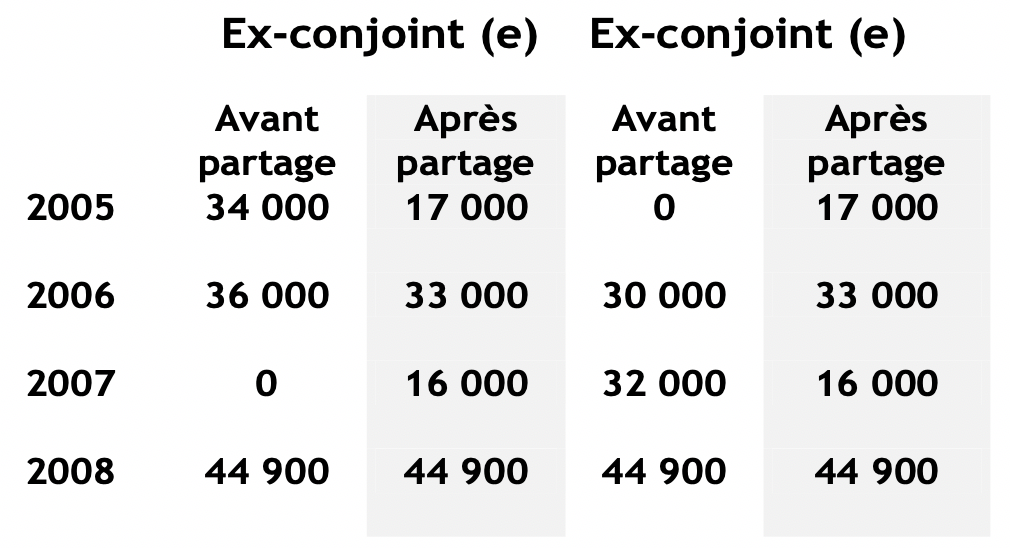
\includegraphics[scale=0.4]{src/ACT-1005/exemple-DIVORCE.png}
\end{center}


\subsubsection*{Division de la rente de retraite}
Conditions:
\begin{itemize}[leftmargin = *]
	\item	Les 2 conjoints doivent avoir au moins 60 ans;
	\item	\hl{L'objectif est l'égalité économique des conjoints};
	\item	La raison principale est fiscale et elle existe depuis 1994;
	\item	Si les conjoints sont mariés, c'est automatique à la demande d'un des deux sinon les deux doivent faire la demande.
\end{itemize}
\textcolor{red}{selon Isabelle, on ne va pas loin sur ce sujet.}


%%%	---------------
%%%	NOTE:
%%%	+	Je ne savais pas trop comment / si je devrais reformuler ces deux prochaines sous-sous-sections parce-que je n'ai pas écris grand chose à propos (AJVR).
%%%	+	Dayum thx big (AJvR)
%%%	---------------
\subsubsection*{Suffisance de la rente}
La PSV et le RRQ fournissent 40\% du salaire (MGA) et l'objectif est d'environ 70\%. Cela est atteint avec des RCR, l'épargne personnelle, etc. Le gouvernement tentera de pallier à ce manque avec l'instauration du régime supplémentaire 1 (1er Janvier 2019).

\subsubsection*{Provisionnement}

Le provisionnement est l'accumulation de la différence entre les entrées et les sorties de fonds (réserve).
\begin{itemize}
\item Dans notre cas, on a un mélange entre un régime par répartition (sans réserve) et un régime à capitalisation (avec réserve)
\item ça emmène un autre type de revenu : le rendement sur les actifs financiers.
\item un régime par répartition emmène quelques problèmes en lien avec la démographie: 
\begin{itemize}
\item On ne peut pas bonifier le régime à cause de la population vieillissante qui va amplifier les problèmes du régime.
\item On est forcer d'augmenter les cotisations à cause de la population vieillissante, faisant en sorte que les retraités actuels auront une rente pour laquelle ils n'ont pas contribués.
\end{itemize}
\end{itemize}


\columnbreak

\subsection*{Régime supplémentaire}
\begin{rappel_enhanced}[Historique]
Entrée en vigueur:
\begin{description}
	\item[Premier volet]	1er janvier 2019 (régime S1);
	\item[Deuxième volet]	1er janvier 2024	(régime S2).
\end{description}
\end{rappel_enhanced}

\begin{conceptgen}{But}
\begin{itemize}[leftmargin = *]
	\item	Améliorer la qualité de vie des futurs retraités au Québec;
	\item	Assurer \hl{l'équité intergénérationnelle};
	\item	Harmoniser le RRQ avec le RPC;
	\item	Renforcer le financement du régime.
\end{itemize}
\end{conceptgen}

\begin{conceptgen}{Financement}
Le régime est \hl{obligatoire} et est en surplus du régime de base.

\begin{description}
	\item[S1]	Pourcentage applicable aux gains entre l'exemption générale et le MGA;
		\begin{itemize}[leftmargin = *]
		\item	La cotisation est équitablement séparée entre l'employeur et l'employé;
		\item	Va augmenter de 0.3\% en 2019 jusqu'à 2\% en 2023.
		\end{itemize}
	\item[S2]	Pourcentage applicable aux gains entre le MGA et le \textbf{MSGA};
		\begin{itemize}[leftmargin = *]
		\item	Le taux est de 8\% (4\% employeur et 4\% employé).
		\end{itemize}
	\item[MSGA]	Le nouveau maximum établit avec le régime supplémentaire.
		\begin{itemize}[leftmargin = *]
		\item	2024 MSGA = $1.07 \times$ MGA;
		\item	2025 MSGA = $1.14 \times$ MGA.
		\end{itemize}
	\item[Fiscalité]		Les cotisations sont déductibles d'impôts.
\end{description}
\end{conceptgen}

\begin{conceptgen}{Prestations}
Toute personne admissible au régime de base est automatiquement admissible au régime supplémentaire. Cependant, le montant de prestation est \hl{proportionnel} au nombre d'années de cotisation.\\

\paragraph*{Taux de remplacement de revenu}
\begin{description}
	\item[S1]	8.33\% de la moyenne des 40 gains admissibles les plus élevés;
	\item[S2]	33.33\% de la moyenne des 40 gains admissibles les plus élevés.
\end{description}


\paragraph*{Proportionnalité}
\begin{itemize}[leftmargin = *]
	\item	Chaque année de participation permet d'accumuler $1/40^{\text{ème}}$ du taux de remplacement de revenu;
	\item	Si on cotise plus de 40 ans, ça permet de sélectionner les 40 années ayant les salaires les plus élevés.
\end{itemize}

Les autres caractéristiques du régime (indexation, partage des droits, etc.) sont comme le régime de base.
\end{conceptgen}

\begin{conceptgen}{Provisionnement}
\begin{itemize}[leftmargin = *]
	\item	Régime capitalisé---les cotisations d'aujourd'hui serviront à payer les prestations des cotisants actuels seulement;
	\item	Il y a donc beaucoup plus d'actifs et les revenus de placements vont représenter la majorité des revenus à long terme;
	\item	Les résultats du régime sont donc plus sensibles au taux de rendement des placements que le régime de base.
\end{itemize}
\end{conceptgen}

\columnbreak

\subsection*{L'invalidité}

\begin{definitionNOHFILL}[Invalide]
\begin{itemize}[leftmargin = *]
	\item	Incapacité grave et permanente;
	\item	Aucune amélioration possible;
	\item	Aucun emploi possible;
	\item	Durée indéterminée.
\end{itemize}

Cette définition est très différente que celle d'une compagnie d'assurance. \\
Par exemple, celle de SSQ:
\begin{center}
	\colorbox{asparagus}{\parbox{0.9\textwidth}{Limitation physique ou mentale, d’une durée temporaire ou permanente, qui empêche un assuré de remplir partiellement ou totalement les principales fonctions de son emploi.}}
\end{center}
\end{definitionNOHFILL}
		
\paragraph*{Note}	Les deux rentes sont payables mensuellement, indexées et imposables.
	
\subsubsection*{Rente d'invalidité}

\begin{conceptgen}{Admissibilité}
\begin{itemize}[leftmargin = *]
	\item	Être déclaré invalide \textit{par la Régie};
		\begin{itemize}[leftmargin = *]
		\item	Évaluation par l'équipe médicale de Retraite Québec.
		\end{itemize}
	\item	Avoir moins de 65 ans;
	\item	Avoir cotisé au moins 2 des 3 dernières années\\
			\textbf{ou}	\\
			5 des 10 dernières années	\\
			\textbf{ou}	\\
			la moitié des toutes les années dans la période cotisable (période d'au moins 4 ans)
\end{itemize}
\end{conceptgen}

\begin{definitionNOHFILL}[Délai de carence]
Période entre le moment où survient l'invalidité et le début des prestations.
\end{definitionNOHFILL}

%%%	----------------------------
%%%	NOTE
%%%	+	manque l'info sur le montant de prestation pour la rente d'invalidité.
%%%	----------------------------

\begin{conceptgen}{Prestation}
\begin{itemize}[leftmargin = *]
	\item	Le paiement est \hl{non-rétroactif} et payable à compter du \hl{quatrième mois suivant celui où le cotisant est reconnu invalide};
	\item	Le paiement cesse lorsqu'il y a :
		\begin{itemize}[leftmargin = *]
		\item	Décès (35\% des cas);
		\item	Cessation d'invalidité (2\% des cas);
		\item	L'obtention de l'âge de 65 ans dans quel cas elle est remplacée par une rente de retraite (63\% des cas).
		\end{itemize}
\end{itemize}
\end{conceptgen}

\subsubsection*{Rente d'enfant de personnes invalides}

\begin{conceptgen}{Admissibilité}
\begin{itemize}[leftmargin = *]
	\item	Cotisant admissible à une rente d'invalidité (RI);
	\item	Enfant du cotisant âgé de moins de 18 ans.
\end{itemize}
\end{conceptgen}

\begin{conceptgen}{Prestation}
\begin{itemize}[leftmargin = *]
	\item	En 2020, paiement mensuel fixe de 79.46\$;
	\item	Le paiement cesse lorsqu'il y a :
		\begin{itemize}[leftmargin = *]
		\item	L'obtention de l'âge de 18 ans par l'enfant;
		\item	Décès de l'enfant;
		\item	Cessation du paiement au cotisant.
		\end{itemize}
\end{itemize}
\end{conceptgen}

\columnbreak

\subsection*{Les prestations de survivants}

\begin{conceptgen}{Admissibilité}
Payable si la personne a décédée a cotisée:
\begin{itemize}[leftmargin = *]
	\item	1/3 des années de sa période cotisable (période d'au moins 3 années)	\\
%%%	--------------------------------
%%%	NOTE
%%%	+	Clarifier ici si c'est 3 ans ou 9 ans période cotisable ?
%%%	--------------------------------
			\textbf{ou}	\\
			10 années.
\end{itemize}
\end{conceptgen}

\subsubsection*{Rente de conjoint survivant}

\begin{definitionNOHFILL}[Conjoint]
\begin{itemize}[leftmargin = *]
	\item	Marriage	\\
			\textbf{ou}\\
			Union civile;
	\item	Conjoint de fait: 3 ans de vie commune (ou 1 s'il y a un enfant);
	\item	Inclut les couples du même sexe.
\end{itemize}
\end{definitionNOHFILL}

\begin{conceptgen}{Prestation}
\begin{itemize}[leftmargin = *]
	\item	Dans le cas d'un remariage, la rente continue d'être versée. \\
			S'il y a décès du nouveau conjoint, la rente la plus avantageuse des deux est versée;
	\item	Les prestations sont mensuelles.
\end{itemize}

Il y a plusieurs composantes à la rente donc certaines qui sont variables (c'est la seule rente avec cette caractéristique).
\begin{itemize}[leftmargin = *]
	\item	La partie uniforme varie selon l'âge et le nombre d'enfants à charge;
	\item	Il est possible que la rente soit réduite si la personne reçoit d'autres rentes (retraite, invalidité) mais est cumulative jusqu'à un maximum établi par la loi.
\end{itemize}
\begin{center}
	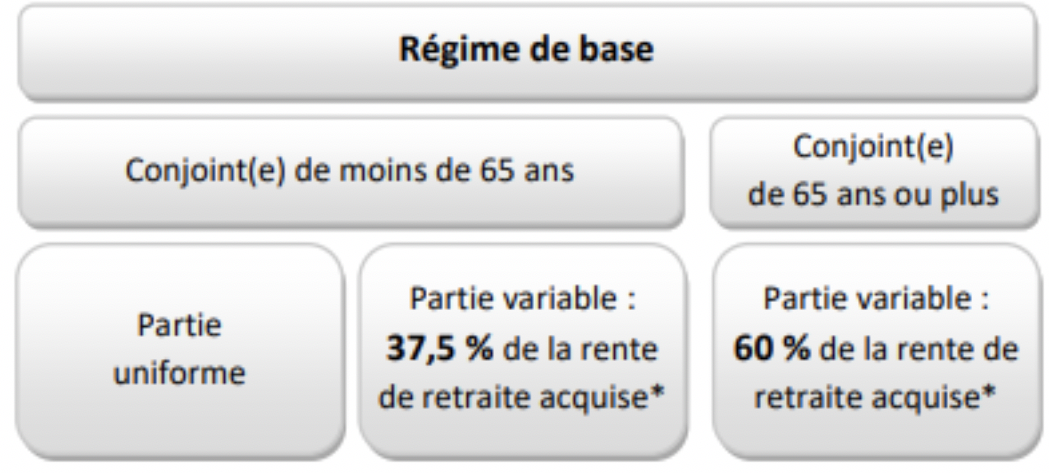
\includegraphics[scale=0.2]{src/ACT-1005/rente-conj-surv.png}
	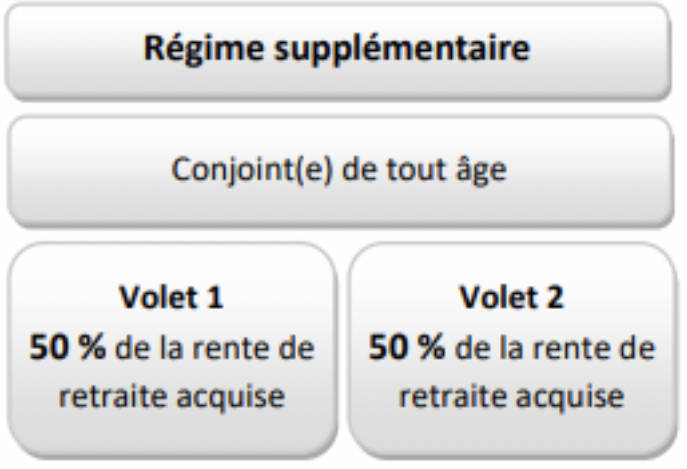
\includegraphics[scale=0.2]{src/ACT-1005/rente-conj-surv-2.png}
\end{center}
\end{conceptgen}

\subsubsection*{Rente d'orphelin}

\begin{conceptgen}{Détails}
\begin{itemize}[leftmargin = *]
	\item	Cesse à 18 ans (ou plus tard s'il est un étudiant à temps plein);
	\item	Montant mensuel fixe \red{(255.03\$ en 2020)};
	\item	Payable une seule fois même si les 2 parents décèdent.
\end{itemize}
\end{conceptgen}

\subsubsection*{Prestation de décès}

\begin{conceptgen}{Détails}
\begin{itemize}[leftmargin = *]
	\item	Montant unique de 2 500\$;
	\item	Priorité à la personne ayant acquitté les frais funéraires.
\end{itemize}
\end{conceptgen}

\newpage

\section{Les régimes volontaires d'épargne retraite (RVER)}

\subsection*{Objectifs}

\subsection*{Obligation d'offrir l'accès à un RVER}


\subsection*{Admissibilité}

\subsection*{Cotisations}

\subsection*{Placements}

\subsection*{Administration}

\subsection*{Fiscalité}

\subsection*{Pistes de réflexion}

\subsection*{Conclusion}

\subsection*{Exemple}

\newpage

\section{Les régimes complémentaires de retraite (RCR)}

Les compagnies peuvent mettre en place et offrir à leurs employés un régime de retraite qui vient en complément des régimes offerts par l'état. 

\begin{definitionNOHFILL}[Définition du RCR]

\begin{description}[leftmargin = *]
	\item[Globalement] Contrat en vertu duquel le participant bénéficie d'une prestation de retraite dont le financement est assuré soit par l'employeur uniquement ou l'employeur et le participant.
	\item[Selon la loi] Le principal objet doit être le paiement d'une rente viagère de retraite aux participants pour les services qu'ils ont accomplis à titre d'employés.
\end{description}

\paragraph{Notes}
\begin{itemize}[leftmargin = *]
	\item	Traditionnellement, ce sont surtout des employés gouvernementaux et de grandes compagnies privées qui ont accès à des RCR---ils sont rares pour les employés de petites entreprises;
	\item	Le gouvernement accorde des avantages fiscaux pour encourager la mise en place de RCR;
	\item	Le fonctionnement est d'accumuler du rendement sur les cotisations pour payer les prestations à la retraite.
\end{itemize}
\end{definitionNOHFILL}
\subsubsection*{Raison d'être}

La raison d'être des régimes complémentaires de retraite est de palier au fait que les rentes gouvernementales n'atteignent pas le 70\% du revenu avant la retraite visée. (sauf pour les faibles revenus)\\
En effet, le RCR a pour but de combler le manque, en emmenant l'épargne directement sur le milieu du travail.

\begin{description}
	\item[Objectif premier:] Fournir un revenu de retraite qui s'ajoute à celui versé par les régimes publics.
	\item[Principe de revenu différé:] C'est quand même de l'argent que l'employeur nous verse, seulement différé.
	\item[Fiscalement:] Pour encourager la mise en place d'un RCR, le gouvernement accorde des avantages fiscaux à l'argent mis de côté dans ces moyens d'épargne-retraite (autant pour les employeurs que les employés s'ils participent).
\end{description}

\subsubsection*{Pour ou contre?}

Point de vue des:
\begin{description}
	\item[Gouvernements]	Les gouvernements les encouragent.
		\begin{itemize}[leftmargin = *]
		\item	Le RCR est un régime \textbf{agréé} car il est \textit{agréé} par la loi pour profiter d'avantages fiscaux;
		\item[$\color{blue}+$]	Utilité sociale des régimes de retraite;
		\item[$\color{blue}+$]	Réduction de la pauvreté parmi les aînés;
		\item[$\color{blue}+$]	Réduction du fardeau de la loi sur la sécurité du revenu;
		\item[$\color{blue}+$]	Accroissement du capital disponible pour investissement dans l'économie;
		\item[$\color{red}-$]	Diminution des revenus fiscaux.
		\end{itemize}
	\item[Entreprises]	L'employeur décide s'il établit un RCR ou non, ainsi que ses modalités et prestations.
		\begin{itemize}[leftmargin = *]
		\item[$\color{blue}+$]	Recrutement et rétention des employés  (Gestion des R-H);
		\item[$\color{blue}+$]	Pression des compétiteurs;
		\item[$\color{blue}+$]	Outil de négociations syndicales;
%%%		--------------------
%%%		NOTE
%%%		+	Vérifier ce que ça veut dire efficacité fiscale. (AJVR)
%%%  + Je suis pas sûr que j'aime la formulation, j'ai mis ce que j'avais noté [OC]
%%%		--------------------
		\item[$\color{blue}+$]	Avantageux fiscalement;
		\item[$\color{blue}+$]	Planification de la retraite des employés simplifiée.
		\item[$\color{red}-$]	Argent non disponible à d'autres fins (e.g., faire grossir la compagnie);
		\item[$\color{red}-$]	Coûts et complexité administrative.
		\end{itemize}
	\item[Employés]	L'employé bénéficie d'un RCR.
		\begin{itemize}[leftmargin = *]
		\item[$\color{blue}+$]	Meilleur revenu de retraite;
%%%		--------------------
%%%		NOTE
%%%		+	Vérifier ce que ça veut dire que les sommes sont provisionnées. (AJVR)
%%% 		+ 	Ça veut dire qu'elles sont capitalisés, qu'elles ne servent pas à la retraite de quelqu'un d'autres, elles sont sécurisés à toi. (OC)
%%%		--------------------
		\item[$\color{blue}+$]	Sécurité des prestations---les sommes sont provisionnées;
		\item[$\color{blue}+$]	Planification de la retraite simplifiée;
		\item[$\color{blue}+$]	Contribution de l'employeur à l'épargne-retraite;
		\item[$\color{red}-$]	Préférence pour un salaire plus élevé plutôt que des prestations de retraite  futures (Avoir l'argent maintenant).
		\end{itemize}
\end{description}

\subsubsection*{Mise en place}
Il n'y a \hl{aucune obligation légale de mettre en place} un régime, \hl{n'y de couvrir tous les employés}. On peut couvrir seulement certains groupes. Cependant, on doit couvrir tous les employés d'une catégorie. Par exemple, on ne peut pas couvrir seulement 3 sur 4 des professeurs d'un département.

\paragraph*{Caractéristiques}	Les dispositions du régime sont déterminées par les compagnies.
\begin{description}
	\item[Participation]	Le régime peut être obligatoire ou facultatif;
		\begin{itemize}[leftmargin = *]
		\item 	S'il est obligatoire, tous les employés de la catégorie visée doivent y adhérer.
		\item	S'il est facultatif, un refus d'y adhérer ne nous fait pas perdre le droit d'y participer plus tard.
		\end{itemize}
	\item[Admissibilité]	Le maximum de temps avant d'être admissible ne peut pas être plus que 2 ans;
	\item[Autres]	La compagnie décide comment gérer:
		\begin{itemize}[leftmargin = *]
		\item	Prestations en cas de décès, cessation d'emploi, d'invalidité;
		\item	La formule de calcul de la rente;
		\item	Les cotisations
		\item	L'âge de retraite sans réduction (Maximum ANR);
		\item	Le service pris en considération;
		\item	Protection contre l'inflation.
		\end{itemize}
\end{description}


\subsubsection*{Contributions}
Les régimes peuvent être:
\begin{description}
	\item[contributifs]	cotisations d'employeurs \textit{et} d'employés.
	\item[non-contributifs]	cotisations seulement des employeurs.
\end{description}

\subsubsection*{Types de régimes}

\paragraph{Note:}	On ne fait qu'énumérer les types de régimes, ils seront tous couverts en détails plus tard.

\begin{description}
	\item[prestations déterminées]	On sait ce qu'on va payer à la retraite, les cotisations sont calculées pour que ça puisse fonctionner.
	\item[cotisations déterminées]	On sait combien on va cotiser, c'est au moment de la retraite qu'on découvre le montant accumulé. 
	\item[hybrides] Un mélange entre les deux types précédents, sera discuté en détail plus tard.
\end{description}

\begin{center}
	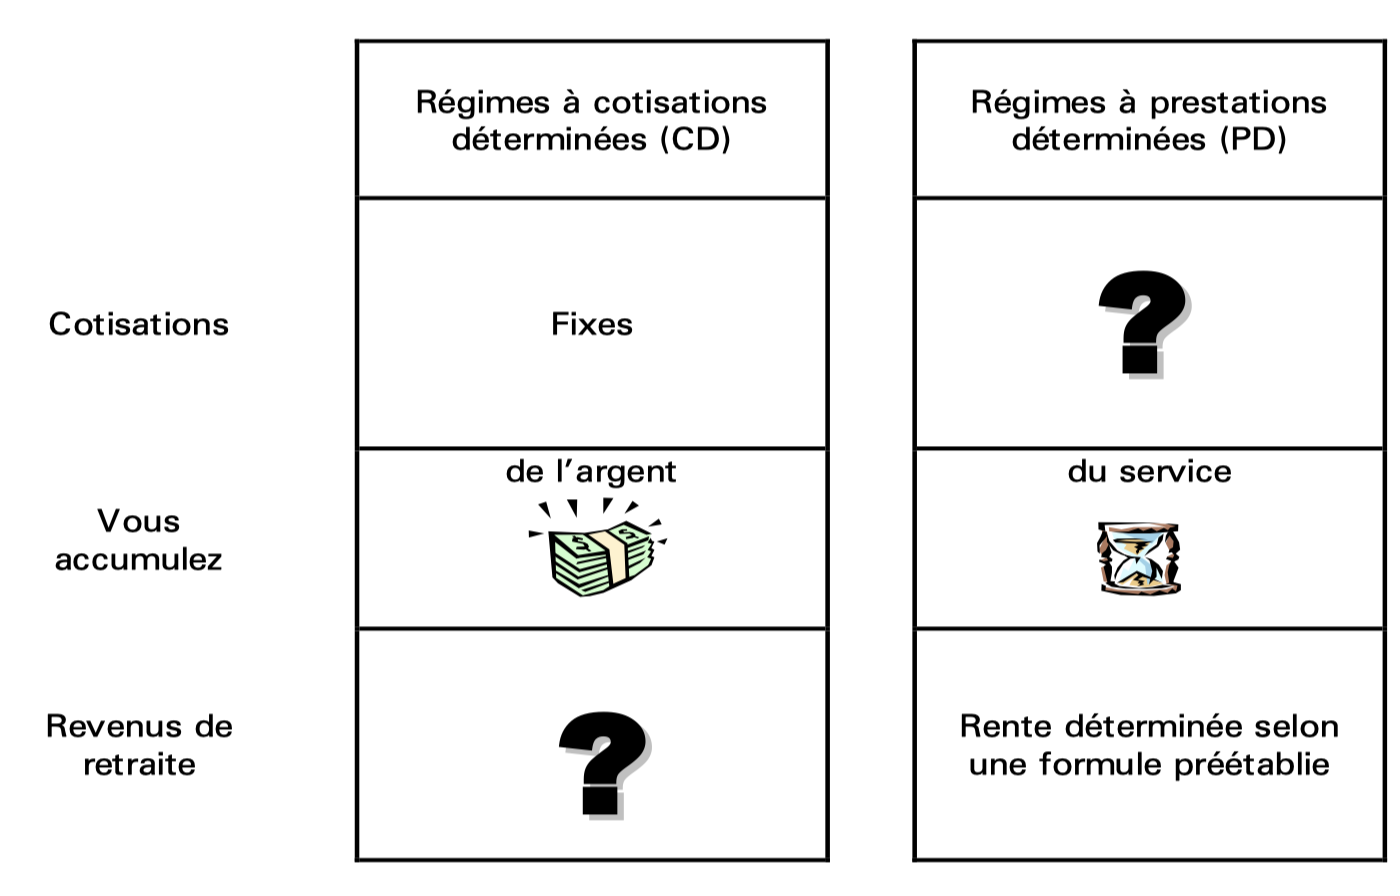
\includegraphics[scale=0.33]{src/ACT-1005/CD-PD-table.png}
\end{center}

\columnbreak

\subsection{Régimes à prestations déterminées (PD)}

\begin{definitionNOHFILL}[Description]
Promesse (pas nécessairement garantie) de payer aux participants un \hl{montant de rente déterminé}.

\paragraph{Notes}
\begin{itemize}[leftmargin = *]
	\item	Le \textit{niveau} des prestations est connu.\\
			C'est-à-dire que la \textit{formule} utilisée pour déterminer les prestations est connue mais \textbf{pas} le \textit{montant} comme tel (même si ça semble pareil);
		\begin{itemize}
		\item	 Exemple : 70\% d'un meilleur salaire qui est aujourd'hui inconnu.
		\end{itemize}
	\item	Le montant varie habituellement selon le nombre d'années de service;
\end{itemize}
\begin{description}
	\item[Années de service]	Période calculée comme le nombre d'années de travail pour un même employeur.
\end{description}
\end{definitionNOHFILL}

\subsubsection*{Financement et investissement}

Le régime est financé par l'employeur (cotisations \textit{patronales}) et, si le régime est contributif, l'employé (cotisations \textit{salariales}).\\

Il n'y a aucune décision d'investissement pour le participant---l'\hl{employeur} investit les cotisations et \hl{c'est lui qui prend les risques d'investissements}. \\

Le provisionnement (capitalisation) est obligatoire (Exigence de la loi sur les RCR) : 
\begin{itemize}
	\item Pour assurer la sécurité des prestations promises;
	\item Pour éliminer les transferts de coût entre les générations;
	\item Ultimement, ça réduit les cotisations requises (rendement sur les sommes accumulés).
\end{itemize}

L'employeur doit être en mesure de payer les prestations futures aux participants du régime et détermine les cotisations patronales (et salariales si contributif) en fonction d'une \textbf{évaluation actuarielle} périodique. 


\begin{definitionNOHFILLsub}[Évaluation actuarielle]
Détermine les cotisations (patronales et salariales s'il y a lieu) requises pour payer les prestations promises selon des \textit{hypothèses prévisionnelles}.

\begin{itemize}[leftmargin = *]
	\item	Exemples d'hypothèses prévisionnelles:
		\begin{itemize}[leftmargin = *]
		\item	Niveau futur des salaires.
		\item	Rendement des placements.
		\item	Moment du départ à la retraite.
		\item	Moment de décès.
		\end{itemize}
	\item	La loi requiert des évaluations aux 3 ans;
	\item	Les objectifs d'une évaluation sont:
		\begin{enumerate}
		\item	Estimer la \textbf{situation financière du régime} à une date donnée;
		\item	Recommander le niveau requis de cotisations;
		\item	Se conformer aux exigences légales.
		\end{enumerate}
\end{itemize}
\end{definitionNOHFILLsub}

\begin{definitionNOHFILLsub}[Situation financière du régime]
Les hypothèses de l'évaluation précédente vont rarement correspondre à la réalité ce qui impact la situation financière.\\

Le régime peut avoir un:
\begin{description}
%%%	--------------------
%%%	NOTE (AJvR)
%%%	+	Faudrait trouver un terme plus simple que "expérience" je trouve ça pourrait throw off du monde d'utiliser un terme actuariel lorsque je ne pense pas que c'est vraiment nécessaire.
%%%	+	J'ai écris ce qui a été observé, qu'est-ce t'en penses?
%%% + 	J'ai modifié ta phrase, quelque chose de plus simple pour quelqu'un en première session peut-être ? On pourra faire un entredeux au besoin, jai conservé la phrase que tu avais fait (OC)
%%%	+	J'aime :) (AJvR)
%%%	--------------------
	\item[Déficit]	Lorsque les choses vont moins bien que prévu et qu'on a une perte (car on aurait reçu des cotisations pas assez élevées pour les coûts qui sont survenus) 
	%selon ce qui a été observé (\textit{l'expérience}).
	\item[Surplus]	Lorsque les choses vont mieux que prévu et qu'on a un gain (car on aurait reçu des cotisations plus élevées pour les coûts qui sont survenus) 
	%selon ce qui a été observé (\textit{l'expérience}).
\end{description}

Exemples d'événements qui peuvent mener à un déficit:
\begin{itemize}[leftmargin = *]
	\item	Niveau futur des salaires---les salaires sont plus élevés que prévu.
	\item	Rendement des placements---les rendements sont moins élevés que prévu.
	\item	Moment de décès---l'espérance de vie augmente.
\end{itemize}


\paragraph{Note} S'il y a un déficit, l'employeur doit verser des cotisations additionnelles pour combler l'écart. Par contre, l'excédent d'\hl{un surplus ne va pas automatiquement à l'employeur} et peut avoir d'autres utilités.
\end{definitionNOHFILLsub}

Les principaux types de régimes à prestations déterminées observés en pratique sont présentés aux boîtes de couleurs qui suivent. 

\subsubsection*{Calcul des prestations de la rente selon un montant fixe forfaitaire}

\begin{definitionNOHFILL}[Prestation forfaitaire]
La rente annuelle est un montant fixe pour chacune des années de service. (Exemple : Chaque mois de service permet d'avoir 100\$ de revenu à la retraite)

Désavantages:
\begin{itemize}
	\item[$\color{red}-$]	Ne tient pas compte du salaire du participant;
	\item[$\color{red}-$]	Les prestations sont en dollars courants et perdent leur pouvoir d'achat s'ils ne sont pas indexés;
	\item[$\color{red}-$]	Pas de notion du remplacement de revenu.
\end{itemize}

Avantages:
\begin{itemize}
	\item[$\color{blue}+$]	Facile à comprendre pour les participants;
	\item[$\color{blue}+$]	Administration simple.
\end{itemize}
\end{definitionNOHFILL}

\subsubsection*{Calcul des prestations de la rente selon un pourcentage du salaire}

La rente est fonction d'un pourcentage de salaire, ou d'une moyenne de salaires, pour chacune des années de service.

Il y a plusieurs types de régimes fonction du pourcentage de salaire.

\begin{definitionNOHFILL}[Salaire de carrière]
La rente est un pourcentage du salaire pour chaque année de participation au régime. \\
La rente payable à la retraite est donc la somme des rentes créditées annuellement durant la carrière du participant.

Désavantages:
\begin{itemize}
	\item[$\color{red}-$]	Les rentes créditées en début de carrière sont un faible pourcentage du salaire final.\\
							Il s'ensuit que c'est moins avantageux s'il y a une progression salariale importante;
	\item[$\color{red}-$]	Puisque la rente n'est pas basée sur des dollars actualisés, le taux de remplacement de revenu peut être inadéquat;
	\item	La revalorisation périodique des rentes créditées serait nécessaire pour atténuer ce problème, mais c'est plus compliqué.
\end{itemize}

Avantages:
\begin{itemize}
	\item[$\color{blue}+$]	Simple à comprendre pour le participant;
	\item[$\color{blue}+$]	Simple à administrer et calculer.
\end{itemize}
\end{definitionNOHFILL}

\begin{conceptgen}{Exemple salaire de carrière}
Formule de rente: 2\% du salaire par année.\\
Adhésion le 1er janvier 2004 et retraite le 1er janvier 2007.
\begin{center}
\begin{tabular}{|	>{\columncolor{airforceblue}}c	| >{\columncolor{beaublue}}c | >{\columncolor{beaublue}}c  |}
\hline\rowcolor{airforceblue} 
\textcolor{white}{\textbf{Année}}	&	\textcolor{white}{\textbf{Salaire}}	&	\textcolor{white}{\textbf{Rente constituée}}		\\\specialrule{0.1em}{0em}{0.0em} 
2004	&	35 000\$	&	700\$	\\
2005&	40 000\$	&	800\$	\\
2006	&	33 000\$	&	860\$	\\\hline
\textbf{Total}	&		&	2 360\$	\\\hline
\end{tabular}
\end{center}
La rente annuelle payable par le régime est 2 360\$.
\end{conceptgen}

\begin{definitionNOHFILL}[Derniers salaires]
La rente est basée sur le nombre d'années de service \textit{et} sur le salaire moyen au cours des $Y$ années précédant la retraite.
\begin{itemize}[leftmargin = *]
	\item	Habituellement 3 ou 5 dernières années;
	\item	Ce sont les prestations les plus généreuses et coûteuses.
\end{itemize}

Désavantages:
\begin{itemize}
	\item[$\color{red}-$]	Administration plus complexe;
	\item[$\color{red}-$]	Coût du régime plus difficile à prévoir;
	\item[$\color{red}-$]	Pénalise les retraites progressives ou changements d'emploi en fin de carrière pour un salaire inférieur (si ce n'est pas prévu au régime).
\end{itemize}

Avantages:
\begin{itemize}
	\item[$\color{blue}+$]	Rente de retraite souvent liée aux meilleurs salaires;
	\item[$\color{blue}+$]	Puisque les augmentations salariales reflètent l'inflation, les rentes aussi.
\end{itemize}

\tcbline

\begin{center}
	\textbf{Salaire meilleurs années}
\end{center}
La rente est la moyenne des $Y$ années de meilleurs salaires. 

\begin{itemize}
	\item	Variante du régime derniers salaires;
	\item	L'avantage additionnel est la correction de l'impact négatif pour les personnes dont le salaire diminue à l'approche de la retraite.
\end{itemize}
\end{definitionNOHFILL}

\begin{conceptgen}{Exemple derniers et meilleurs salaires}
Formule de rente: 2\% $\times$ salaire final moyen sur 3 ans (SFM3) $\times$ années de participation (AP).\\
Adhésion le 1er janvier 1975 et retraite le 1er janvier 2010 (35 ans de service).
\begin{center}
\begin{tabular}{|	>{\columncolor{airforceblue}}c	| >{\columncolor{beaublue}}c |}
\hline\rowcolor{airforceblue} 
\textcolor{white}{\textbf{Année}}	&	\textcolor{white}{\textbf{Salaire}}	\\\specialrule{0.1em}{0em}{0.0em} 
1975		&	21 000\$		\\
\dots	&	\dots		\\
2006		&	70 000\$		\\
2007		&	74 000\$		\\
2008		&	77 000\$		\\
2009		&	65 000\$		\\\hline
\end{tabular}
\end{center}
\textbf{Selon derniers salaires}:
\begin{itemize}
	\item	SFM3 = $\frac{65000\$ + 77 000\$ + 74 000\$}{3} = 72 000\$$.
	\item	Rente annuelle de retraite = $2\% \times 72 000\$ \times 35 \text{ ans} = 50 400\$$.
\end{itemize}

\textbf{Selon meilleurs salaires}:
\begin{itemize}
	\item	SFM3 = $\frac{70 000\$ + 77 000\$ + 74 000\$}{3} = 73 667\$$.
	\item	Rente annuelle de retraite = $2\% \times 73 667\$ \times 35 \text{ ans} = 51 567\$$.
\end{itemize}
\end{conceptgen}

\begin{definitionNOHFILL}[Régimes flexibles]
Permets aux participants de verser des cotisations optionnelles (CO) pour acheter des prestations accessoires (PA) de leur choix.\\

Quelques exemples:
\begin{itemize}[leftmargin = *]
	\item	Bénéfice de décès avant retraite;
	\item	Indexation après la retraite;
	\item	Retraite anticipée sans réduction.
\end{itemize}

Notes
\begin{itemize}[leftmargin = *]
	\item	Les CO sont déductibles d'impôts et ne réduisent pas la marge permise au REER;
	\item[$\color{red}-$]	Administration plus compliquée;
	\item[$\color{blue}+$]	Flexible selon la situation de l'employé.
\end{itemize}
\end{definitionNOHFILL}


\columnbreak
\subsection{Régimes à cotisations déterminées (CD)}

\begin{definitionNOHFILL}[Description]
\hl{Les cotisations} (de l'employeur et l'employé) \textit{ou} la méthode utilisée pour les calculer \hl{sont déterminées à l'avance.}

\paragraph{Notes}
\begin{itemize}[leftmargin = *]
	\item	Comme un compte de banque, la rente est fonction des cotisations. On ne connaitra le montant de la rente qu'à la date de la retraite du participant;
	\item	Puisque le montant dépend de la valeur accumulée des cotisations, le moment de la retraite peut être problématique s'il y a une chute des marchés.
\end{itemize}
\end{definitionNOHFILL}


\subsubsection*{Investissement}

L'\hl{employé assume le risque d'investissement} puisque son revenu à la retraite est directement lié au rendement du compte ayant les cotisations. \\

Il s'ensuit 	qu'il est généralement responsable du choix de placement et qu'il peut le changer en tout temps. \\

Puisque le but d'un régime à cotisations déterminées n'est pas de payer une rente de retraite, l'employé devra transférer le montant accumulé dans son compte pour ensuite l'emmener dans un autre véhicule financier destiné au paiement d'une rente de retraite. 

\begin{definitionNOHFILLsub}[Véhicules financiers destinés au paiement d'une rente]
Le montant accumulé peut être transféré dans un:
\begin{description}
	\item[Compte de retraite immobilisé (CRI)]	L'équivalent d'un REER auquel on peut transférer des fonds provenant d'un RCR sauf qu'ils sont immobilisés.
		\begin{itemize}[leftmargin = *]
		\item	Le compte sert donc uniquement à accumuler de l'épargne-retraite.
		\item	Pour en tirer un revenu, l'individu doit soit transférer les sommes à un FRV ou acheter une rente viagère d'un assureur.
		\end{itemize}
	\item[Fonds de revenu viager (FRV)]	Fonds enregistré de revenu de retraite (FERR).
		\begin{itemize}[leftmargin = *]
		\item	Le fonds a une \textbf{limite} du montant pouvant être retiré annuellement.
		\item	Les sommes proviennent soit d'un CRI ou directement d'un RCR.
		\end{itemize}
	\item[Une rente]d'un assureur variant selon:
		\begin{itemize}[leftmargin = *]
		\item	le montant accumulé;
		\item	le taux d'intérêt de l'assureur (au moment du transfert);
		\item	l'âge du rentier (et co-rentier s'il y a lieu);
		\item	la forme (viagère ou différée) et les garanties de la rente.
		\end{itemize}
\end{description}
\end{definitionNOHFILLsub}

\paragraph{Note}	Les régimes à CD ont le danger que le cotisant n'ait pas assez de revenus à la retraite. Ceci peut être dû à un faible taux de cotisation salariale, un rendement faible du fonds de placement par défaut, etc.

\subsubsection*{Types de formule pour calculer les prestations de rentes}

\begin{definitionNOHFILL}[Cotisation déterminées]
Les cotisations sont: 
\begin{itemize}[leftmargin = *]
	\item	un pourcentage fixe du salaire \\
			\textbf{ou}
	\item	un montant donnée par années de service\\
			\textbf{ou}
	\item	un montant donnée par heure travaillé
\end{itemize}
\end{definitionNOHFILL}

\begin{conceptgen}{Exemple cotisation déterminée}
\begin{description}
	\item[Salaire]	40 000\$
	\item[Service]	22 ans
	\item[Cotisation de l'employé] 4\% de son salaire	
\end{description}
\tcbline
Exemple 1: 
\begin{description}
	\item[Taux de cotisation de l'employeur]	3\% du salaire;
	\item[Cotisation de l'employeur]	= 40 000\$ $\times$ 3\% = 1 200\$.
\end{description}	 
	
\tcbline

Exemple 2: 
\begin{description}
	\item[Taux de cotisation de l'employeur]	= taux de l'employé = 4\% du salaire;
	\item[Cotisation de l'employeur]	= 40 000\$ $\times$ 4\% = 1 600\$;
	\item[$\color{blue}+$]	Lorsque l'employeur cotise de façon égale à l'employé cela incite l'épargne.
\end{description}
	
\tcbline

Exemple 3: taux de cotisation de l'employeur selon une table:
\begin{center}
\begin{tabular}{|	>{\columncolor{white}}c	| >{\columncolor{white}}c |}
\hline\rowcolor{airforceblue} 
\textcolor{white}{\textbf{Années de service $x$}}	&	\textcolor{white}{\textbf{Rapporté}}	\\\specialrule{0.1em}{0em}{0.0em} 
$x \le$ 10 ans	&	75\%	\\
10 ans $< x <$ 20 ans	&	100\%	\\
$x \ge$ 20 ans	&	125\%	\\\hline
\end{tabular}
\end{center}
\begin{description}
	\item[Taux de cotisation de l'employeur]	= taux de l'employé $\times$ 1.25 = 4\% $\times$ 1.25 = 5\% du salaire;
	\item[Cotisation de l'employeur]	= 40 000\$ $\times$ 5\% = 2 000\$;
	\item[$\color{blue}+$]	Reconnait le service,
\end{description} 
\end{conceptgen}

\begin{definitionNOHFILL}[Avec participation aux bénéfices]
Les cotisations de l'employeur sont liées à la rentabilité de l'entreprise.

\begin{itemize}[leftmargin = *]
	\item	L'agence du revenu du Canada (ARC) exige que l'entreprise verse un minimum de 1\% de la masse salariale. (même dans les années de faible rentabilité)
	\item	La répartition se fait selon une formule basée sur les années de service et/ou le salaire.
\end{itemize}

Désavantages:
\begin{itemize}
	\item[$\color{red}-$]	Augmente l'incertitude liée au montant de rente;
\end{itemize}

Avantages:
\begin{itemize}
	\item[$\color{blue}+$]	Peut motiver les employés à être plus productifs.
\end{itemize}
\end{definitionNOHFILL}

\begin{definitionNOHFILL}[Régime simplifié]
Régime à CD administré par un établissement financier offert aux employeurs (mélange de CD et REER).

\begin{itemize}[leftmargin = *]
	\item	Ce régime est un mélange de fonds immobilisés et non immobilisés. \\
			Les cotisations de l'employeur et de l'employé (à moins d’avis contraire de l’employeur) sont immobilisées. \\
			Les cotisations additionnelles de l'employé sont non immobilisées.
\end{itemize}
\end{definitionNOHFILL}


\columnbreak
\subsection{Résumé des différents RCR}

\subsubsection*{Régime à prestations déterminées (PD)}
\begin{center}
	\textbf{Employé}
\end{center}
Pour
\begin{itemize}
	\item[$\color{blue}+$]	Permets de comprendre la notion de remplacement de revenus.
	\item[$\color{blue}+$]	L'employeur assume le risque de placement.
	\item[$\color{blue}+$]	Bon pour les employés avec beaucoup d'années de service.
	\item[$\color{blue}+$]	Les cotisations salariales sont déductibles d'impôts. (S'il y en a)
	\item[$\color{blue}+$]	Les cotisations optionnelles (CO) permettent d'optimiser la valeur fiscale.
	\item[$\color{blue}+$]	Possibilité de racheter des années de service antérieures.
\end{itemize}

Contre
\begin{itemize}
	\item[$\color{red}-$]	Plus compliqué à comprendre.
	\item[$\color{red}-$]	Fonds immobilisés non disponibles pour autre chose.
	\item[$\color{red}-$]	Le facteur d'équivalence (FE) réduit les marges au REER.
\end{itemize}

\begin{center}
	\textbf{Employeur}
\end{center}
Pour
\begin{itemize}
	\item[$\color{blue}+$]	Développement des programmes de retraite pour gérer la fluctuation de la main-d'œuvre (retraite anticipée).
	\item[$\color{blue}+$]	Possibilité d'augmenter les prestations au besoin.
	\item[$\color{blue}+$]	Premier bénéficiaire des gains sur les rendements et l'expérience (surplus).
	\item[$\color{blue}+$]	Cotisations patronales déductibles d'impôts.
\end{itemize}

Contre
\begin{itemize}
	\item[$\color{red}-$]	Coût d'administration plus élevé.
	\item[$\color{red}-$]	Difficile de prévoir la charge de retraite et impossible de prévoir le coût réel du régime.
	\item[$\color{red}-$]	Plus de communication est nécessaire.
\end{itemize}

\subsubsection*{Régime à cotisations déterminées (CD)}
\begin{center}
	\textbf{Employé}
\end{center}
Pour
\begin{itemize}
	\item[$\color{blue}+$]	Facile à comprendre.
	\item[$\color{blue}+$]	Flexibilité des placements.
\end{itemize}


Contre
\begin{itemize}
	\item[$\color{red}-$]	Employé assume le risque d'investissement avant \textbf{et} après sa retraite.
	\item[$\color{red}-$]	Le montant de prestation de retraite n'est pas prévisible.
\end{itemize}

\begin{center}
	\textbf{Employeur}
\end{center}
Pour
\begin{itemize}
	\item[$\color{blue}+$]	Tenue de dossiers simple.
	\item[$\color{blue}+$]	Coûts facilement budgétisés.
	\item[$\color{blue}+$]	Aucun risque d'investissement.
%%%	--------------------
%%%	NOTE (AJvR)
%%%	+	Pas sur de ce que ça veut dire exactement / pourquoi c'est une bonne chose?
%%%	+	Me semble la compagnie ne serait pas contente d'avoir des fonds immobilisés puisqu'elle ne peut pas faire un rendement d'investissement / l'utiliser pour expansion / etc.?
%%% + 	Je suis d'accord avec toi ! C'est un avantage dans la mesure ou l'employé ne pourra pas aller au casino avec l'argent que l'employeur souhaite lui donner pour la retraite. (OC)
%%%	+	Ah je catch, merci :) (AJvR)
%%%	--------------------
	\item[$\color{blue}+$]	L'argent sera utilisé pour la retraite (immobilisation)
		\begin{itemize}
		\item	Ceci est un avantage pour l'employeur, car ça assure que l'employé ne pourra pas utiliser les fonds pour autre chose que sa retraite.
		\end{itemize}
\end{itemize}

Contre
\begin{itemize}
	\item[$\color{red}-$]	Administration des RCR réglementés.
%%%	--------------------
%%%	Voir note ci-dessus
%%%	--------------------
	\item[$\color{red}-$]	Pas d'outils pour gérer les ressources humaines. (On ne peut pas contrôler les retraites anticipés)
%%%	--------------------
%%%	NOTE
%%%	+	Pourquoi c'est un négatif pour eux?
%%%	+	Ce ne serait pas uniquement un négatif pour les employés ou est-ce que je manque de quoi ici?
%%%	+	J'ai l'impression que c'est parce que on peut pas nécéssairement Dire aux employés qu'on va leur donner un meilleur revenu... on peut juste cotiser plus. Ça parle moins directement aux employés.  (OC)
%%%	+	lol 10-4, merci (AJvR)
%%%	--------------------
	\item[$\color{red}-$]	Montant de prestation non-prévisible.
	\item[$\color{red}-$]	Certaine responsabilité sur les (mauvais) placements des employés et donc le besoin des informer sur le risque/rendement des placements.
	\item[$\color{red}-$]	Prestations peuvent être inadéquate pour les employés déjà âgés.
\end{itemize}

\newpage

\subsection{Hybrides}

\begin{definitionNOHFILL}[Description]
Régime à cotisations \textbf{et} prestations déterminées; les cotisations ainsi que la méthode du calcul de la rente sont prédéterminées.
\end{definitionNOHFILL}

\subsubsection*{Types de formule pour calculer les prestations de rentes}

\begin{definitionNOHFILL}[Cotisations et prestations déterminées]
Verse le maximum entre la \textcolor{teal}{rente à PD} et \textcolor{teal}{la rente pouvant être souscrite des cotisations accumulées}.


Désavantages:
\begin{itemize}
	\item[$\color{red}-$]	Plus d'administration par l'employeur qui doit gérer les investissements.
\end{itemize} 

Avantages:
\begin{itemize}
	\item[$\color{blue}+$]	Réduis l'incertitude d'un régime à CD, car il y garantit un revenu minimal à la retraite;
	\item[$\color{blue}+$]	Détermine si c'est un régime à PD ou CD seulement au moment de la retraite.
\end{itemize}
\end{definitionNOHFILL}

\begin{definitionNOHFILL}[Combiné]
Additionne les rentes de la composante à PD et de la composante à CD

\begin{itemize}[leftmargin = *]
	\item	Souvent l'employeur fournit la composante à PD et l'employé la composante à CD.
\end{itemize}

Désavantages:
\begin{itemize}
	\item[$\color{red}-$]	Complexe à administrer et expliquer.
\end{itemize}
\end{definitionNOHFILL}


\columnbreak
\subsection{Autres caractéristiques}

\subsubsection*{Coordination avec les régimes d'État}
\paragraph{Note:}	Le RCR tient compte du RRQ/RPC.\\

Les régimes d'état ont un maximum de contribution selon le MGA. Alors, \textbf{pour les salaires inférieurs au MGA}:
\begin{itemize}[leftmargin = *]
	\item	Les cotisations au RCR seront plus faibles afin de tenir compte des cotisations que  l'employé verse déjà;
	\item	Les prestations versées par le RCR seront moindres afin de tenir compte des prestations que l'employé reçoit déjà.
\end{itemize}

\subsubsection*{Enregistrement et fiscalité}
Les RCR sont (obligatoirement) enregistrés auprès des organismes de réglementation.

Chaque province a une loi sur les RCR. \\
Au Québec, la loi régit:
\begin{itemize}[leftmargin = *]
	\item	Les participants à un régime de retraite dans la province;
	\item	La conformité des régimes;
	\item	La diffusion d'information pour renseigner ses membres.
\end{itemize}
\begin{description}
	\item[Note]	Retraite Québec est responsable de l'administration de cette loi au Québec. 
\end{description}

\

Au niveau fédéral il y a la loi de l'impôt sur le revenu (LIR).
\begin{itemize}[leftmargin = *]
	\item	La loi prévoit un traitement favorable à l'impôt des RCR pour les encourager.
	\item	Les cotisations ne sont pas imposables, mais les prestations le sont lorsqu'elles sont versées.
	\item	Fondée selon le principe que tous les contribuables ayant le même revenu devraient bénéficier du même niveau d’aide fiscale à l’épargne retraite.\\
			Et cela, peu importe le mode d’épargne retraite utilisé (RCR, RVER, REÉR, \dots);
	\item	Il y a donc une \hl{limite globale d'aide fiscale} qui vise \textbf{tous} les modes d'épargne retraite;
	\item	Présentement, c'est 18\% du salaire de l'année précédente (sujet à un montant maximal également);
	\item	On a donc introduit le \textbf{facteur d'équivalence (FE)}.
\end{itemize}

\begin{definitionNOHFILL}[Facteur d'équivalence (FE)]
Le \textbf{facteur d'équivalence} représente la valeur présumée de la participation de l'année précédente au régime de retraite de l'employeur. Il sert à égaliser les retraités qui bénéficient d'un RCR à ceux qui n'en n'ont pas.

\begin{itemize}[leftmargin = *]
	\item	Le montant réduit la limite globale de cotisation aux REER/RVER;
	\item	Pour les régimes à PD, c'est une formule en fonction de la rente constituée durant l'année;
	\item	Pour les régimes à CD, c'est la somme des cotisations (patronales et salariales).
\end{itemize}
\end{definitionNOHFILL}

La LIR a été réformée en 1991


\subsubsection*{Âge d'admissibilité à la retraite}
Âge auquel on a prévu commencer à verser la rente sans réduction actuarielle

\begin{itemize}[leftmargin = *]
	\item	Habituellement, cet âge est l'ANR de 65 ans;
	\item	Cependant, certains régimes prévoient un ANR \textit{inférieur} à 65 ans, mais aucun ne peut prévoir un âge \textit{supérieur};
	\item	Certains régimes peuvent se baser sur un certain nombre d'années de service, ou un mélange d'âge et de nombre d'années de service;
	\item	Il y a possibilité d'une retraite 10 ans avant l'âge d'admissibilité (avec réduction actuarielle).
\end{itemize}


\subsubsection*{Prestations de décès avant la retraite}
\begin{itemize}[leftmargin = *]
	\item	Il est obligatoire pour le régime de définir les prestations que le conjoint, ou autres, recevront si le participant décède avant sa retraite.
	\begin{itemize}
	\item	Pour payer les frais funéraires;
	\item 	Car l'assuré a quand même contribué toute sa vie...
	\end{itemize}
	\item	Le montant de prestation doit être, au minimum, égal aux sommes versées accumulées du participant;
%%%	------------------------
%%%	NOTES
%%%	+	Quoi? (AJVR)
%%% +	Hypothèse : Pour que ce conjoint puisse utiliser ces fonds pour sa retraite à lui. Ça pourrait être à poser sur le forum. (OC)
%%%	+	hmmm intéressante hypothèse j'ai posé la question; à voir. (AJvR)
%%%	------------------------
	\item	immobilisé si le survivant est un conjoint (pour sa retraite à lui?)
	\item	Normalement un seul paiement forfaitaire.
\end{itemize}

\subsubsection*{Prestations de décès pendant la retraite}
\begin{itemize}[leftmargin = *]
	\item	Loi prévoit le versement d'une rente de survivant au conjoint admissible du retraité;
	\item	Doit être d'au moins 60\% de la rente du retraité et se surnomme donc une "\textbf{rente réversible}";
	\item	Versée même si le conjoint se remarie.
\end{itemize}

\paragraph{Note}	La loi n'oblige pas de protéger la rente contre l'inflation avec une indexation post-retraite.


\newpage
\section{Accidents du travail et maladies professionnelles}

\begin{conceptgen}{Santé et sécurité au travail (SST)}
Programme d'assurance sociale (type Bismarck) pour couvrir les accidents du travail et la maladie professionnelle. 
\begin{itemize}[leftmargin = *]
	\item	Au Canada c'est une couverture provinciale.
	\item	2 rôles:
		\begin{description}
		\item[Assureur public]	rôle traditionnel d'un assureur, soit compenser une perte lorsqu'elle survient.
		\item[Agent de prévention]	rôle additionnel de faire de la prévention du risque.
		\end{description}
\end{itemize}
\end{conceptgen}


\subsection{Historique}
\subsubsection*{Fin du 19e siècle}

Contexte historique:
\begin{itemize}[leftmargin = *]
	\item	La perception des accidents au travail était qu'ils font partie des risques inhérents au travail;
	\item	Le travailleur devait donc en supporter la responsabilité et les conséquences;
	\item	L'approche était que plus le travail était risqué, plus le salaire serait élevé (C'était la seule forme de \textit{protection salariale}).
\end{itemize}

\begin{rappel_enhanced}[\shortstack{Factory and Workshop Act\\ (1879 en Angleterre)}]
Objectif est de mettre fin à l'\textit{exploitation} des femmes et des enfants.

\begin{itemize}[leftmargin = *]
\item	On était pas rendu à régler la problèmatique des accidents de travail, on s'occupe d'abord de l'exploitation.
\end{itemize}
\end{rappel_enhanced}

\begin{rappel_enhanced}[\shortstack{Acte des manufactures\\ (1885 au Québec)}]
L’objectif est de \textit{protéger} la vie et la santé des femmes et des enfants au travail. C'est également la première fois qu'on parle de \textit{prévention}, mais toujours pas de \textit{compensation}.
\begin{itemize}[leftmargin = *]
	\item	Fixer l'âge minimum à l'embauche.
	\item	Premières règles sur la sécurité la maladie.
	\item	Tournées obligatoires de médecins.
	\item	Approbation municipale obligatoire de l'usine avant sa construction.
\end{itemize}
\end{rappel_enhanced}

Lorsqu'un travailleur était victime d'un accident de travail :
\begin{itemize}
\item On considérait que c'était à lui de supporter les conséquences financières qui en découlent car ça fait partie des risques inhérents au travail;
\item L'accidenté devait intenter un procès pour prouver la responsabilité de l'employeur (si c'était le cas). C'était au travailleur analphabète que revenait le fardeau de la preuve.
\end{itemize}

\subsubsection*{Fin du 20e siècle}

Contexte historique:
\begin{itemize}[leftmargin = *]
	\item	Période d'industrialisation;
	\item	Les accidents de travail sont plus fréquents;
	\item	Les tribunaux ne sont plus suffisants pour gérer tous les accidents de travail et les recours ne sont ni justes ni équitables;
	\item	La perception du marché de travail et des juges est: si un ouvrier ne fait pas attention, il est normal qu'il paie pour sa négligence;
	\item	Cela dit, les accidents ne viennent pas uniquement de négligence, mais aussi d'endroits de travail non sécuritaires.
\end{itemize}

Événements:
\begin{itemize}[leftmargin = *]
	\item	Institution d'une commission pour enquêter comment les autres pays régissent la responsabilité des employeurs pour les accidents de travail (Ontario en 1910);
	\item	L'Ontario devient ensuite la première province à adopter une loi, Loi sur les accidents de travail, et de créer une commission des accidents de travail en 1914;
	\item	Les autres provinces adoptent graduellement des lois: en 1915 la Nouvelle-Écosse, en 1916 le Manitoba et la Colombie-Britannique, en 1918 le Nouveau-Brunswick, en 1929 le Saskatchewan et au Québec en 1931;
	\item	Cette loi mène au nouveau \hl{régime québécois d'indemnisation des victimes d'accidents au travail}.	\\
			Les travailleurs victimes d'une \textbf{lésion professionnelle} sont indemnisés et les employeurs, en contrepartie, bénéficient d'un régime collectif d'assurance responsabilité \textbf{sans égard à la faute}.
\end{itemize}

Dans le temps, la loi était basée sur 5 éléments (encore présents aujourd'hui, mais pas tous au même niveau):
\begin{enumerate}
	\item	Couverture sans égard à la responsabilité (no fault);
		\begin{itemize}[leftmargin = *]
		\item	En échange d'indemnités automatiques en cas de blessure, les travailleurs ont renoncé à tout droit de poursuite;
		\item	Donc que ce soit la faute du travailleur ou de l'employeur, aucune poursuite.
		\end{itemize}
	\item	Responsabilité collective;
		\begin{itemize}[leftmargin = *]
		\item	En échange d'être dégagé de toute poursuite en cas de blessure, les employeurs financent le programme collectivement.
		\end{itemize}
	\item	Indemnités garanties;
		\begin{itemize}[leftmargin = *]
		\item	Le montant et paiement est garanti sur le plan legislatif;
		\end{itemize}
	\item	Administration indépendante;
		\begin{itemize}[leftmargin = *]
		\item	Administration libre de tout groupe de pression potentiel de travailleurs, d'employeurs ou du gouvernement (Ce sera la CNESST).
		\end{itemize}
	\item	Juridiction exclusive.
		\begin{itemize}[leftmargin = *]
		\item	Au lieu d'aller aux tribunaux, une contestation d'indemnisation se fait dans une commission dite "quasi judiciaire".
		\end{itemize}
\end{enumerate}


\subsubsection*{Aujourd'hui}
Deux lois en vigueur:

\begin{rappel_enhanced}[\shortstack{Loi sur la santé et\\ la sécurité du travail (1979)}]
Axée sur la prévention.
\end{rappel_enhanced}

\begin{rappel_enhanced}[\shortstack{Loi sur les accidents de travail et\\ les maladies professionnelles (1985)}]
Ajoute la réparation (indemnisation) et la réadaptation.
\end{rappel_enhanced}

La \textbf{C}ommission des \textbf{n}ormes, de l'\textbf{é}quité, de la \textbf{s}anté et de la \textbf{s}écurité du \textbf{t}ravail (CNESST) est maintenant l'organisme qui gère l'administration du régime.


\columnbreak
\subsection{Accidents de travail et Maladies professionnelles}
\begin{definitionNOHFILL}[Accidents de travail]
Événement: 
\begin{itemize}[leftmargin = *]
	\item	Imprévu et soudain, 
	\item	Attribuable à toute cause, 
	\item	Survenant à une personne par le fait, ou à l'occasion, de son travail et qui entraîne pour elle une lésion professionnelle.
\end{itemize}
\

Le dommage subi doit être apparu de façon soudaine, par exemple: 
\begin{itemize}[leftmargin = *]
	\item	Chute;
	\item	Blessure avec un outil;
	\item	Intoxication;
	\item	Lésions cervicales;
	\item    etc.
\end{itemize}
\end{definitionNOHFILL}

\begin{definitionNOHFILL}[Maladie professionnelle]
Maladie :
\begin{itemize}[leftmargin = *]
	\item	contractée par le fait, ou à l'occasion, du travail,
	\item	qui est caractéristique, ou reliée directement aux risques particuliers, de ce travail.
\end{itemize}
\

Exemple de maladies:
\begin{description}
	\item[reconnues]	Amiantose, tendinite, etc.
	\item[non reconnues]	Épuisement (difficile à relier au travail, rarement compensé)
\end{description}
\end{definitionNOHFILL}

Pour qu'il y ait un accident du travail, il faut qu'il y ait un \hl{fait accidentel} et qu'il ai entraîné une \hl{lésion professionnelle}.

\begin{definitionNOHFILL}[Lésion professionnelle]
\textbf{Blessure}, ou \textbf{maladie}, qui survient par le fait, ou à l’occasion, d’un accident du travail, ou maladie professionnelle. Donc, il doit y avoir une relation de cause à effet et non seulement une coïncidence entre l'accident et la lésion.\\

Il y  est compris: 
\begin{itemize}[leftmargin = *]
	\item	la récidive, 
	\item	la rechute et 
	\item	l’aggravation.
\end{itemize}

La loi pose une \textit{présomption} qu'un accident qui arrive lorsque le travailleur est sur les lieux à son travail \textit{est} une lésion professionnelle.\\
Le travailleur n'a donc qu'a démontrer les éléments de la présomption pour recevoir l'indemnité \textit{\textbf{mais}} l'employeur peut contester les faits.
\end{definitionNOHFILL}

\begin{definitionNOHFILL}[Fait accidentel]
Pour qu'il y ait un accident du travail, il faut d'abord qu'il y ait un fait accidentel. Il s'agit d'un événement qui survient \textbf{soudainement} et qui se produit d'une manière \textbf{imprévue}. \\

Un accident peut résulter de gestes faits en exécutant un travail, comme un effort soutenu et inhabituel ou même un geste qui pourrait être répréhensible, tant qu'il ne s'agit \textbf{pas} d'une \textbf{négligence grossière et \textit{volontaire}} de la part du travailleur.
\end{definitionNOHFILL}

L'événement peut se produire:
\begin{description}
	\item[Par le fait du travail]	il survient lorsque le travailleur exécute ses tâches et est directement lié au travail;
	\item[À l'occasion du travail]	il ne survient pas nécessairement lorsque le travailleur exécute ses tâches \textit{habituelles}, mais les activités exercées sont connexes au travail.
		\begin{itemize}[leftmargin = *]
		\item	Dans un tel cas, le lien d'\textbf{autorité} entre l'employeur et le travailleur détermine si c'est un accident de travail---si le travailleur suivait des consignes ou était sous la supervision de l'employeur;
		\item	Les circonstances, le lieu et le moment de survenance de l'accident sont également pris en compte.
		\end{itemize}
\end{description}

%\subsection{Régime sans égard à la responsabilité}

%%%	--------------------
%%%	NOTES (AJvR)
%%%	+	Je n'ai pas défini ici puisque c'est déjà fait dans les 5 éléments fondamentaux plus haut.
%% 	+	Je suis d'accord. (OC)
%%%	--------------------

\begin{definitionNOHFILLsub}[Couverture]
Tout travailleur avec quelques exceptions prévues par la loi:
\begin{itemize}[leftmargin = *]
	\item	Les employeurs;
	\item	Les travailleurs autonomes;
	\item	Les athlètes professionnels;
	\item	Les bénévoles;
	\item	Les personnes engagées (par un particulier) pour garder une autre personne (enfant, personne âgée, etc.).
\end{itemize}

Conditions:
\begin{itemize}[leftmargin = *]
	\item	Le travailleur est obligatoirement couvert automatiquement et ne cotise pas pour être protégé (l'employeur cotise).\\
			Cela dit, on considère quand même la couverture comme étant bismarckienne puisque ce sont les travailleurs qui sont couverts et, même si elles viennent de l'employeur, il y a des contributions.
	\item	L'accident est couvert s'il survient au Québec;
	\item	La maladie est couverte si elle est contractée au Québec.
\end{itemize}
\end{definitionNOHFILLsub}

\begin{definitionNOHFILLsub}[Prévention]
Tout employeur, sous peine de lourdes amendes, doit:
\begin{itemize}[leftmargin = *]
	\item	\textbf{Prévenir} les accidents;
	\item	\textbf{Fournir} des \textbf{appareils} de sécurité et de premiers soins;
		\begin{itemize}[leftmargin = *]
		\item	Par exemple, une machine pour se laver les yeux de produits chimiques (appareil de sécurité).
		\end{itemize}
	\item	\textbf{Maintenir} des \textbf{services} de premiers soins.
		\begin{itemize}[leftmargin = *]
		\item	Par exemple, former des travailleurs en premiers soins.
		\end{itemize}
\end{itemize}

La CNESST:
\begin{itemize}[leftmargin = *]
	\item	soutient les travailleurs, et employeurs, dans leurs démarches pour améliorer la sécurité du milieu de travail;
	\item	Inspecte les lieux de travail.
\end{itemize}
\end{definitionNOHFILLsub}

\begin{definitionNOHFILLsub}[Indemnisation]
Objectifs:
\begin{itemize}[leftmargin = *]
	\item	Maintenir la rémunération et les avantages au même niveau que si l’employé était au travail;
	\item 	Protéger l’intégrité financière du conjoint et des enfants à charge suite à la perte du revenu de l’employé.
\end{itemize}

4 \textbf{types} généraux de prestations :
\begin{itemize}
\item	Indemnité de remplacement de revenu;
\item	Indemnité pour préjudice corporel;
\item 	Indemnité au décès;
\item	Autre.
\end{itemize}
\end{definitionNOHFILLsub}

\begin{definitionNOHFILL}[Indemnité de remplacement de revenu]
Calcul:
\begin{description}
	\item[1er jour]	Travailleur reçoit 100\% de son salaire \textbf{net} de son employeur pour la partie de la journée où manquée.
		\begin{itemize}[leftmargin = *]
		\item	La CNESST ne rembourse pas l'employeur.
		\end{itemize}
	\item[14 premiers jours (complets) d'incapacité]	Travailleur reçoit 90\% du salaire net de l'employeur jusqu'à concurrence du maximum annuel assurable.
		\begin{itemize}[leftmargin = *]
		\item	La CNESST veut encourager le retour au travail sans toutefois interrompre le salaire.\\
				Alors, le travailleur continue à recevoir son salaire moins une légère pénalité;
		\item	Le maximum annuel assurable est le montant maximal que la CNESST va accepter de remplacer.\\
				En 2019, ce montant était de 76 500\$ et est indexé annuellement;
		\item	\textbf{Note}: La CNESST va rembourser ce montant à l'employeur (que la réclamation soit acceptée ou pas).
		\end{itemize}
	\item[15e jour (complet) d'incapacité]	Suite au calcul, il y a prise en charge par la CNESST.
\end{description}

\tcbline

Notes:
\begin{itemize}[leftmargin = *]
	\item	Les prestations sont indexées au coût de la vie;
	\item	L'indemnité prend fin au premier des événements suivants:
		\begin{itemize}[leftmargin = *]
		\item	Capacité à exercer son emploi;
		\item	Décès;
		\item	68e anniversaire de naissance.
		\end{itemize}
\end{itemize}
\end{definitionNOHFILL}

\begin{algo2}[\shortstack{Étapes du calcul de l'indemnité de\\ remplacement de revenu}]
\begin{enumerate}[leftmargin = *]
	\item	Déterminer la période des 14 premiers jours complets;
		\begin{itemize}[leftmargin = *]
		\item	Ce sont les \hl{14 premiers jours \textbf{de calendrier} et non de travail}.
		\end{itemize}
	\item	Déterminer le nombre de jours payables
		\begin{itemize}[leftmargin = *]
		\item	Jours auxquels le travailleur aurait normalement travaillé;
		\item	Il y a des cas faciles (e.g. lundi au vendredi) et compliqués (e.g. remorqueur).
		\end{itemize}
	\item	Déterminer le salaire \textbf{brut} et le salaire maximum assurable pour la période;
		\begin{itemize}[leftmargin = *]
		\item	Le salaire brut inclut: bonis, pourboires, heures supplémentaires, etc.
		\end{itemize}
	\item	Calculer le salaire net du travailleur;
		\begin{itemize}[leftmargin = *]
		\item	Donc, on calcule le net du minimum entre le salaire brut et le salaire maximum assurable.
		\end{itemize}
	\item	Calculer l’indemnité à verser au travailleur.
		\begin{itemize}[leftmargin = *]
		\item	Verser 90\% du salaire net pour les jours payables.
		\end{itemize}
\end{enumerate}

\paragraph{Note}	Il y a un exemple à la page 31 du PPT du cours sur la SST.
\end{algo2}

\begin{definitionNOHFILL}[Indemnités pour préjudice corporel]
Indemnité pour préjudice corporel pour une personne qui, en raison d'un accident de travail ou d'une maladie professionnelle, subit un dommage physique ou psychique permanent. Cette indemnité tient compte de:
\begin{itemize}[leftmargin = *]
	\item	De la sévérité du handicap (aussi appelé le \textit{déficit anatomo-physiologique});
	\item	Du préjudice esthétique;
	\item	Des douleurs et de la perte de jouissance de la vie.
\end{itemize}

Notes
\begin{itemize}[leftmargin = *]
	\item	C'est un montant forfaitaire.
	\item	Calcul: 
	\setlength{\mathindent}{-1.5cm}
		\begin{align*}
		\left(\shortstack{\% de l'atteinte\\ permanente}\right)	\times	\left(\shortstack{montant correspondant \\ à l'âge de la personne}\right)
		\end{align*}
	\setlength{\mathindent}{1cm}
			L'âge de la personne est déterminée selon le \textit{moment où survient} la lésion.
	\item	Le montant maximal (en 2017) varie de dans les alentours de 100 000\$ pour 18 ans et moins à 50 000\$ pour 65 ans et plus mais ils sont revalorisés annuellement.
\end{itemize}
\paragraph{Note}	Il y a un exemple à la page 36 du PPT du cours sur la SST.
\end{definitionNOHFILL}

\begin{definitionNOHFILL}[Indemnité au décès]
Indemnité versée au aux personnes ayant un lien de dépendance économique avec le travailleur au moment de son décès.

Il y a plusieurs cas (e.g. conjoints ou enfants invalides) mais les plus importants sont:

\textbf{Conjoint survivant}
\begin{itemize}[leftmargin = *]
	\item	Droit à une indemnité mensuelle, forfaitaire et des frais de funérailles;
	\item	L'indemnité mensuelle est versée pendant un à trois ans et équivaut à 55\% de l'indemnité de remplacement de revenu à laquelle le travailleur aurait droit.\\
			Son maximum est de 2 137.64\$ par mois;
	\item	L'indemnité forfaitaire, selon l'âge du conjoint, est de un à trois fois le salaire annuel du défunt.
\end{itemize}

\textbf{Enfant mineur}
\begin{itemize}[leftmargin = *]
	\item	Droit à une rente mensuelle jusqu'à sa majorité afin d'assurer une sécurité de revenu;
	\item	Rente de 542\$ par mois.
\end{itemize}

Notes:
\begin{itemize}
	\item	Les indemnités de décès sont revalorisées annuellement.
\end{itemize}
\end{definitionNOHFILL}

\begin{definitionNOHFILL}[Autres indemnités]
\begin{itemize}[leftmargin = *]
	\item	Coût de remplacement de vêtements abimés lors de l'accident de travail;
	\item	Coût de prothèses et orthèses;
	\item	Coût de médicaments et soins médicaux non-couverts par les programmes publics.
\end{itemize}
\end{definitionNOHFILL}


\columnbreak
\subsection{Tarification}
La CNESST est entièrement financée par les cotisations des employeurs.\\

La prime, comme toute autre assurance, varie selon la:
\begin{description}
	\item[Fréquence]	Le risque associé aux activités de l'employeur;
	\item[Sévérité]	Coût des lésions.
\end{description}

On regroupe les employeurs en \textbf{groupes de tarifications} selon: 
\begin{itemize}[leftmargin = *]
	\item	La similarité des activités exercées;
	\item	La nature des accidents;
	\item	Les dangers susceptibles d'en découler.
\end{itemize}

Le groupe se fait imposer un taux de cotisation, en \% de la masse salariale, qui doit être suffisant pour couvrir:
\begin{itemize}[leftmargin = *]
	\item	Le coût d'indemnités approximatif pour la prochaine année;
	\item	Les frais administratifs et liés à la prévention;
	\item	Les déficits/surplus de l'année précédente.
\end{itemize}

En 2019, ce taux était de 1.79\$ par 100\$ de masse salariale admissible.

Le taux peut être personnalisé selon le type d'entreprise. Il y a 3 types de personnalisation:
\begin{description}
	\item[Taux de l'unité]	S'applique pour les petites entreprises ($\approx 72\%$ des employeurs);
		\begin{itemize}[leftmargin = *]
		\item	Représente le risque de l'ensemble des employeurs---c'est une gestion collective;
		\item	Puisque l'entreprise est petite, il n'y a pas assez d'événements pour la tarifier directement.
		\end{itemize}
	\item[Taux personnalisé]	S'applique aux moyennes et grandes entreprises selon leur expérience ($\approx 27\%$ des employeurs); 
		\begin{itemize}[leftmargin = *]
		\item	Le taux de l'unité est ajusté pour tenir des efforts de l'entreprise à promouvoir la prévention et la facilité de réadaptation;
		\end{itemize}
	\item[Rétrospective]	S'applique aux très grandes entreprises ($\approx 1\%$ des employeurs).
		\begin{itemize}[leftmargin = *]
		\item	La cotisation est ajustée en fonction de l'évolution sur 4 ans des coût des lésions professionnelles.
		\end{itemize}
\end{description}

Les petites et moyennes entreprises n'ont pas accès au même niveau de personnalisation, mais peuvent se regrouper pour former une \textbf{mutuelle de prévention}.

\begin{definitionNOHFILL}[Mutuelle de prévention]
Regroupement d’employeurs qui décident font des démarches pour favoriser la prévention des lésions professionnelles, la réadaptation et le retour en emploi afin de bénéficier d’une tarification reflétant leurs efforts. La mutuelle est une entité qui gère l'ensemble des employeurs et produit des bilans.
\tcbline
Notes:
\begin{itemize}[leftmargin = *]
	\item	L'adhésion est facultative; 
	\item	Aucun lien est nécéssaire entre les employeurs;
	\item	Un employeur "magasine" pour une mutuelle afin de la rejoindre;
	\item	Chaque employeur doit créer et appliquer un programme de prévention et le mettre à jour annuellement;
	\item	Le taux d'un employeur est déterminé selon les masses salariales et prestations de tous les employeurs de la mutuelle;
	\item	Puisqu'elle reflète l'expérience, une mutuelle ne mène pas nécessairement à une réduction de la prime, mais une mutuelle efficace devrait mener à une baisse de la prime.
\end{itemize}
\end{definitionNOHFILL}


\columnbreak
\subsection{Fiscalité}
Les cotisations patronales sont déductibles d'impôts.
Les indemnités versées ne sont pas imposables puisqu'elles sont calculées avec le salaire net.

%\columnbreak
\subsection{Coordination}
\subsubsection*{Régimes privés}
\begin{description}
\item[Régimes collectifs :]	La CNESST est le premier payeur et le régime collectif paiera ce qui dépasse pour arriver à sa promesse.
\item[Régimes individuels]	En sus, (selon le contrat) je pourrais recevoir le double de compensation (Aucune coordination).
\end{description}

\subsubsection*{Régimes publics}
Certaines factures sont transférées à la CNESST. 



\newpage
\section{La Politique familiale et le régime québécois d’assurance parentale (RQAP)}
\subsection{Objectifs}
L'objectif principal est d'aider les familles à assurer les besoins essentiels des enfants; en particulier, les familles avec de faibles revenus. (Mesure d'assistance sociale)\\

En particulier:
\begin{itemize}[leftmargin = *]
	\item	Inciter la procréation;
	\item	Soit faciliter la décision de rester à la maison, ou promouvoir la participation des femmes sur le marché du travail;
	\item	Appuyer le développement des enfants.
\end{itemize}


\subsection{Historique}

\begin{description}
	\item[1918]	Programme \textcolor{bulgarianrose}{fédéral} "\textit{exemption pour les enfants}";
	\item[1945]	Programme \textcolor{bulgarianrose}{fédéral} d'allocations familiales;
		\begin{itemize}[leftmargin = *]
		\item	Montant par enfant âgé de 16 ans ou moins, avec réduction à partir du 5e enfant;
		\item	La mentalité était encore que le montant devait être versé au père pour conserver l'autorité sur les familles.
		\end{itemize}
	\item[1954]	Premier programme \textcolor{blue(pigment)}{québécois};
		\begin{itemize}[leftmargin = *]
		\item	Exemptions fiscales.
		\end{itemize}
	\item[1967]	Programme \textcolor{blue(pigment)}{québécois} d'allocations familiales;
		\begin{itemize}[leftmargin = *]
		\item	Favorise les familles nombreuses avec des montants croissants à chaque enfant;
		\item	Prestations universelles en surplus du programme \textcolor{bulgarianrose}{fédéral}.
		\end{itemize}
	\item[1970]	Ajout de prestations de maternité au programme \textcolor{bulgarianrose}{fédéral} d'assurance emploi;
	\item[1974 à 1997]	Transition d'un programme universel à un programme d'assistance sociale avec des allocations plus élevées pour les familles à faibles revenus;
	\item[1986]	Politique nataliste;
		\begin{itemize}[leftmargin = *]
		\item	Indice de fécondité: Niveau de remplacement des générations passe de 5.3 enfants par femme en 1920 à 1.63 en 1980 à 1.39 en 1985;
		\item	Natalité est un enjeu important avec 500\$ pour le premier enfant, 1000\$ pour le deuxième et 8000\$ pour le troisième;
		\item	Pas d'impact visible à long terme;
		\item	Aboli en 1997.
		\end{itemize}
	\item[1997]	Révision majeure de la politique familiale \textcolor{blue(pigment)}{québécoise};
		\begin{itemize}[leftmargin = *]
		\item	Un vieillissement démographique imminent va mener à une raréfaction de la main d'œuvre;
		\item	Les femmes seront nécessaires pour le marché du travail et donc l'idée de garderies à 5\$ commence à s'élaborer.
		\end{itemize}
	\item[2006]	Entrée en vigueur du \textbf{\textcolor{blue(pigment)}{RQAP}} (finalement);
	\item[Aujourd'hui]	Au niveau:
		\begin{description}
		\item[\textcolor{bulgarianrose}{fédéral}]	Allocation canadienne pour enfants selon le revenu (pas universel).
		\item[\textcolor{blue(pigment)}{québécois}]	Aide aux parents (allocations familiales);
		\item[\textcolor{blue(pigment)}{québécois}]	Services de garde subventionnés;
		\item[\textcolor{blue(pigment)}{québécois}]	RQAP.
		\end{description}
\end{description}


\columnbreak
\subsection{RQAP}

C'est un régime de remplacement de revenu avec des prestations:
\begin{multicols*}{2}
\begin{itemize}[leftmargin = *]
\item	de maternité;
\item	de paternité (rare);
\item	parentales;
\item	d'adoption.
\end{itemize}
\end{multicols*}

\textbf{Notes}:
\begin{itemize}[leftmargin = *]
	\item	Pour un résident du \textcolor{blue(pigment)}{Québec}, ça remplace la portion maternité du programme d'assurance emploi \textcolor{bulgarianrose}{fédéral};
	\item	Les prestations sont imposables, mais les cotisations à verser au régime sont déductibles d'impôts;
	\item	Le conseil de gestion de l'assurance parentale, sous le ministre du Travail, de l'Emploi et de la Solidarité sociale, est en charge du RQAP.
\end{itemize}

\subsubsection*{Accessibilité}
\begin{itemize}[leftmargin = *]
	\item	Puisque c'est un régime de \textit{remplacement de revenu}, on doit avoir travaillé pour y avoir accès (Lié au travail---Bismark);
	\item	Le revenu minimum admissible est de 2 000\$, peut donc couvrir les étudiants et travailleurs à temps partiel.
\end{itemize}

\subsubsection*{Prestations}
\textbf{Niveau des prestations}:
\begin{itemize}[leftmargin = *]
	\item	Le revenu maximum admissible est élevé à 78 500\$ en 2020 (même niveau que la CNESST);
	\item	Les prestations remplacent jusqu'à 75\% du revenu hebdomadaire moyen;
	\item	Comparativement, l'assurance-emploi remplace 55\% du revenu hebdomadaire jusqu'à un maximum de revenu admissible de 54 200\$.
\end{itemize}

\textbf{Paiement des prestations}:
\begin{itemize}[leftmargin = *]
	\item	Il n'y a pas de délai (de carence) avant de recevoir les prestations;
	\item	Le parent peut choisir entre recevoir un \textbf{régime de base} ou un \textbf{régime particulier};
	\item	En 2018, 3/4 des Québécois ont choisi le régime de base;
	\item	En 2018, il y a eu 73 834 demandes de prestations sur 83 800 nouveaux-nés---il faut être un travailleur pour faire la demande;
	\item	Un \textit{régime de base} a des prestations moins élevées pour plus longtemps et le \textit{régime particulier} des prestations plus élevées pour moins longtemps:
\end{itemize}

\begin{center}
	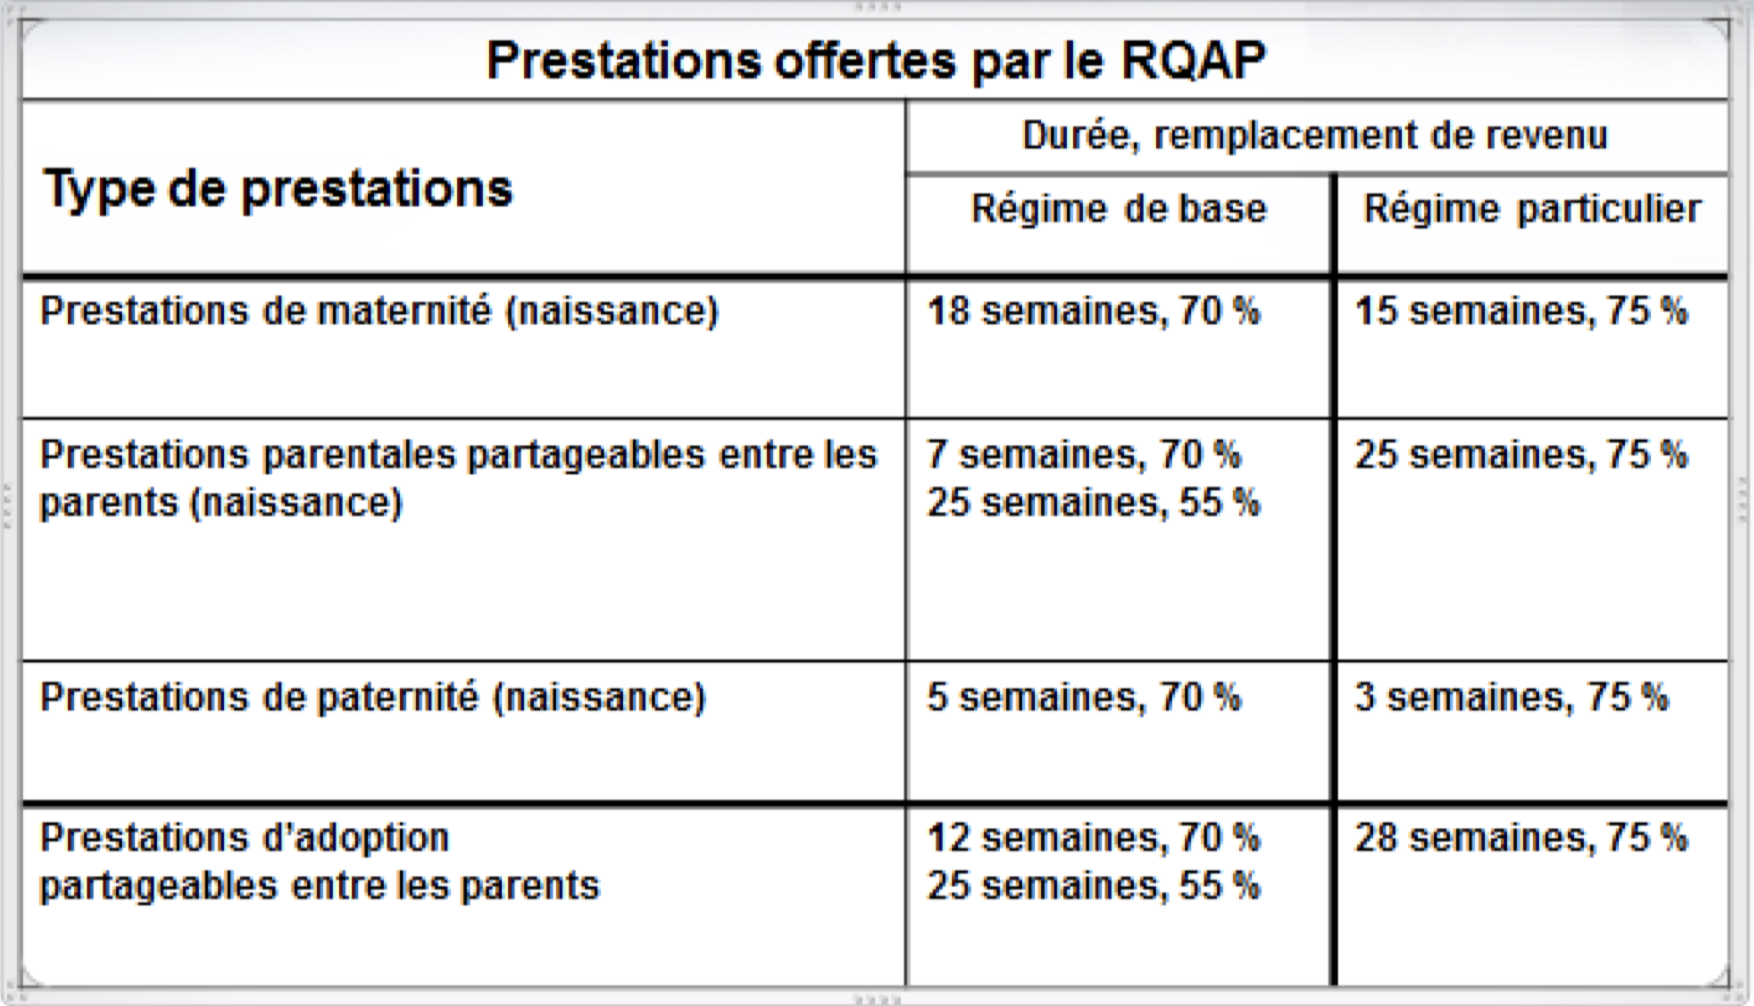
\includegraphics[scale=0.25]{src/ACT-1005/RQAP-prestations.png}
\end{center}


\subsubsection*{Cotisations}

\begin{center}
\begin{tabular}{| >{\columncolor{beaublue}}p{1.8cm}	| >{\columncolor{beaublue}}c  | >{\columncolor{beaublue}}c  |}
\hline\rowcolor{airforceblue} 
\textcolor{white}{\textbf{Type de cotisants}}	&	\parbox[t]{2cm}{\textcolor{white}{\textbf{Taux de\\ cotisation (2019$\rightarrow$2020)}}}	&	\parbox[t]{2cm}{\textcolor{white}{\textbf{Cotisations\\ maximales (2019$\rightarrow$2020)}}}		\\\specialrule{0.1em}{0em}{0em} 
Salariés	&	0.526\%	$\rightarrow$ 0.494\%	&	402.39\$	$\rightarrow$ 387.79\$	\\\hline
Employeurs	&	0.736\%	$\rightarrow$ 0.692\%	&	563.04\$$\rightarrow$ 534.22\$	\\\hline
Travailleurs autonomes	&	0.934\%	$\rightarrow$ 0.878\%		&	714.59 $\rightarrow$ 689.23\$	\\\hline
\end{tabular}
\end{center}

\begin{itemize}[leftmargin = *]
	\item	Le programme fédéral d'assurance-emploi ne couvre plus les prestations de maternité, parentales, et d'adoption pour les Québécois;
	\item	Alors, les Québécois ont un rabais sur leurs cotisations à l'assurance-emploi:
\end{itemize}

\begin{center}
\renewcommand{\arraystretch}{1.5}
\begin{tabular}{| >{\columncolor{beaublue}}m{3cm} | >{\columncolor{beaublue}}l  |}
\hline\rowcolor{airforceblue} 
\textcolor{white}{\textbf{Type de cotisants}}	&	\parbox[c]{4cm}{\textcolor{white}{\textbf{Rabais 2019},\\ (\% du salaire assurable)}}		\\\specialrule{0.1em}{0em}{0em} 
Salariés	&	0.37\%	\\\hline
Employeurs	&	1.4 $\times$ \shortstack{rabais\\ salarié} $=$ 0.518\%	\\\hline
Travailleurs autonomes	&	0.37\%	\\\hline
\end{tabular}
\end{center}


\subsection{Comparaison internationale du RQAP}
\begin{description}
	\item[Congé maternité]	Programme courant, plusieurs pays qui remplacent près de 100\% du salaire;
		\begin{itemize}
		\item	Allemagne, Croatie, Serbie, etc.
		\end{itemize}
	\item[Congé paternité]	Programme rare dont le Canada est exemplaire.
\end{description}


\subsection{Impacts de la mise en place du RQAP}
\begin{itemize}[leftmargin = *]
	\item	Jusqu'en 2006, le taux de natalité était toujours plus grand au Canada, mais le Québec a surpassé le Canada depuis;
	\item	Cela dit, le taux décroît au Québec depuis 2012;
	\item	Augmentation de l'activité physique chez les pères;
	\item	(Faible) réduction de la dépression et anxiété chez les mères;
	\item	Atténuation de l'inégalité des genres. 
\end{itemize}


\columnbreak
\subsection{Projets de loi}

\begin{definitionNOHFILLsub}[Projet de loi 174]
Présenté le 22 mars 2018, mais jamais adopté.\\

\textbf{Propositions :}
\begin{itemize}[leftmargin = *]
	\item	Possibilité d'étaler le congé actuel sur 2 ans;
	\item	D'exclure certaines semaines à faibles revenus de la période de référence dans le calcul des prestations;
	\item	Possibilité de constituer une banque de congés (de 5 ou 10 jours) avec les prestations non versées;
	\item	Créer des prestations exclusives pour chacun des parents adoptants et augmenter le nombre de semaines de prestations d'adoption;
	\item	Offrir des prestations de maternité pendant plus de semaines lors d'une grossesse multiple.
\end{itemize}
\end{definitionNOHFILLsub}

\begin{definitionNOHFILLsub}[Projet de loi 51]
Déposé en fin 2019, si c'est adopté ce sera applicable aux enfants nés à partir du 1er janvier 2020.\\

\textbf{Propositions :}
\begin{itemize}[leftmargin = *]
	\item	Augmenter la durée des prestations (nouveau-nés et adoptions);
	\item	Accorder des semaines de prestations additionnelles si \textbf{chacun} des parents reste à la maison avec leur enfant un minimum de semaine afin d'encourager les pères à passer plus de temps auprès du bébé;
		\begin{description}
		\item[Régime de base]	Si chacun des parents prend au moins 10 semaines des congés parentaux, on ajoute 4 semaines de congé;
		\item[Régime particulier]	Si chacun des parents prend au moins 8 semaines, on en ajoute 4.
		\end{description}
	\item	Ajout de semaines de congé lorsqu'il y une grossesse multiple ou une adoption de plusieurs enfants (5 pour le régime de base et 3 pour le régime particulier);
	\item	Retrait de 5 semaines \textit{à partager} et ajout de 5 semaines pour chacun des parents;
	\item	Le nombre à partager passe donc au même nombre de semaines (32) que les parents naturels;
	\item	Augmentation du maximum de salaire que l'on peut gagner tout en recevant les prestations parentales.
\end{itemize}
\end{definitionNOHFILLsub}



\newpage
\section{L’assurance emploi}

\begin{definitionNOHFILLsub}[Objectifs]
Fournir de l'aide financière temporaire aux chômeurs canadiens qui:
\begin{itemize}[leftmargin = *]
	\item	Ont perdu leur emploi sans en être responsables,
	\item	Cherchent un nouvel emploi ou perfectionnent leurs compétences.
\end{itemize}

\

\textbf{Particulièrement avec des prestations :}
\begin{description}
	\item[régulières]	Les chômeurs;	
	\item[de maladie]	Les travailleurs malades;
	\item[de pêcheur]	Les pêcheurs indépendants;
	\item[de compassion]	Les personnes qui doivent s'occuper d'un membre de leur famille atteint d'une maladie grave;
	\item[de maternité]	Les femmes enceintes;
	\item[parentales]	Les parents de nouveau-nés / nouvellement adoptés;
	\item[\textit{Note}:]	Ces deux dernières sont remplacées par l'assurance parentale au Québec.
\end{description}
\end{definitionNOHFILLsub}


\columnbreak
\subsection{Historique}
\begin{description}
	\item[1935]	La Loi sur le placement et les assurances sociales est déclarée inconstitutionnelle puisque les domaines ne relèvent pas exclusivement du gouvernement fédéral;
	\item[1940]	Accord unanime parmi toutes les provinces d'accorder le pouvoir au gouvernement fédéral de concevoir un régime d'assurance-chômage (10 juillet);
	\item[1940]	Loi \textcolor{bulgarianrose}{fédérale} sur l'assurance-chômage (7 août);
		\begin{itemize}[leftmargin =*]
		\item	But est de fournir un soutien du revenu temporaire aux particuliers en chômage.
		\end{itemize}
	\item[1945]	Soulève la préoccupation d'assister les prestataires dans la recherche d'emploi;
		\begin{itemize}[leftmargin =*]
		\item	Modifications graduelles au fil du temps.
		\end{itemize}
	\item[1971]	Adoption de la nouvelle loi sur l'assurance-chômage;
		\begin{itemize}[leftmargin =*]
		\item	Assouplit les conditions d'admissibilité au régime;
		\item	Augmente le montant des prestations.
		\end{itemize}
	\item[1996]	Loi sur l'assurance-emploi remplace la loi sur l'assurance-chômage;
		\begin{itemize}[leftmargin =*]
		\item	Plus récente grande réforme, le nom est maintenant en lien avec le but du régime (promouvoir l'emploi);
		\item	But de combiner le soutien du revenu et l'aide à l'emploi dans une même loi.
		\end{itemize}
	\item[2008]	Création de l'Office de financement de l'assurance-emploi du Canada.
		\begin{itemize}[leftmargin =*]
		\item	Administré par Service Canada afin d'accroître l'indépendance à établir le taux de cotisation et s'assurer que les cotisations servent exclusivement aux fins du régime.
		\end{itemize}
\end{description}


\columnbreak
\subsection{Cotisations}
\textbf{Notes}:
\begin{itemize}[leftmargin = *]
	\item	Elles sont requises de la part des employeurs et employés;
	\item	Il n'y a pas d'âge minimal ou maximal;
	\item	Certains des programmes spéciaux sont financés par le gouvernement directement au lieu des cotisations.
\end{itemize}

\textbf{Taux}:
\begin{itemize}[leftmargin = *]
	\item	Taux de cotisation des employés:
		\begin{itemize}[leftmargin = *]
		\item	\textcolor{bulgarianrose}{Canada}:  En 2020, taux de 1.58\% de la rémunération assurable avec un maximum de 54 200\$.
		\item	\textcolor{blue(pigment)}{Québec}:  En 2020, taux de 1.20\% de la rémunération assurable (Revoir RQAP pour comprendre d'où vient notre rabais).
		\end{itemize}
	\item	Le taux des employeurs est 1.4 fois celui des employés;
	\item	Il paye plus puisqu'il a plus de contrôle sur les mises à pied.
\end{itemize}

\textbf{Cotisation annuelle}:
\begin{itemize}[leftmargin = *]
	\item	Certifiée par l'actuaire en chef annuellement;
	\item	Le taux d'équilibre est recherché sur une période de 7 ans;
	\item	Le but est qu'il n'y ait pas d'excédents à placer et que les cotisations servent uniquement à financer l'assurance emploi.
\end{itemize}


\columnbreak
\subsection{Prestations}
\subsubsection*{Caractéristiques}
\begin{itemize}[leftmargin = *]
	\item	Délai de carence de 1 semaine;
		\begin{itemize}[leftmargin = *]
		\item	Était 2 semaines avant 2017;
		\item	Les prestations parentales n'ont pas de délai (Il doit être assez rare qu'on la demande pour de faux bébés).
		\end{itemize}
	\item	La prestation équivaut à 55\% de la rémunération hebdomadaire assurable (jusqu'au maximum).
\end{itemize}

\subsubsection*{Types de prestations}
\begin{definitionNOHFILL}[Prestations régulières---chômage]
\paragraph{Admissibilité}
\begin{itemize}[leftmargin = *]
	\item	Présenter une demande de prestations;
	\item	Être en arrêt de travail non volontaire (exclus : démissions sans justification, être congédié pour inconduite, grève, etc.);
	\item	Être prêt à travailler;
	\item	Avoir occupé un emploi assurable pendant un nombre minimal d'heures pendant la période de référence.
\end{itemize}

\paragraph{Période de référence}
La plus courte période entre:
\begin{itemize}[leftmargin = *]
	\item	52 semaines;
	\item	La période depuis le début d'une période de prestations antérieures.
\end{itemize}

\paragraph{Nombre minimal d'heures d'emploi assurables}
420 à 700 heures selon le taux de chômage de la région. \\
Au extrêmes, pour un taux de chômage de:
\begin{itemize}[leftmargin = *]
	\item	6\% ou moins, 700 heures;
	\item	13.1\% ou plus, 420 heures.
\end{itemize}

\paragraph{Période de prestation}
14 à 45 semaines selon :
\begin{itemize}[leftmargin = *]
	\item	Le taux de chômage de la région;
	\item	Le nombre d'heures d'emploi (assurable) accumulées au cours de la période de référence.
\end{itemize}
\end{definitionNOHFILL}

\begin{definitionNOHFILL}[Prestations de maladie]
\paragraph{Admissibilité}
\begin{itemize}[leftmargin = *]
	\item	Personnes incapables de travailler soit en raison d'une blessure ou d'une maladie;
	\item	La rémunération doit avoir diminué d'au moins 40\%.
\end{itemize}

\paragraph{Période de référence}
Même définition que le chômage.

\paragraph{Nombre minimal d'heures d'emploi assurables}
Au moins 600 heures accumulées durant la période de référence.

\paragraph{Période de prestation}
Maximum de 15 semaines.
\end{definitionNOHFILL}

\begin{definitionNOHFILL}[Prestations de compassion]
\paragraph{Admissibilité}
\begin{itemize}[leftmargin = *]
	\item	Personnes qui doivent s'absenter du marché du travail pour \og \textit{offrir des soins ou du soutien}\fg{} à un membre de la famille souffrant d'une maladie grave qui risque d'en décéder;
	\item	\og \textit{offrir des soins ou du soutien} \fg{}:
		\begin{itemize}[leftmargin = *]
		\item	Offrir un support psychologique ou émotionnel;
		\item	S'arranger pour trouver quelqu'un d'autre pour prodiguer des soins;
		\item	Fournir directement des soins.
		\end{itemize}
	\item	La rémunération doit avoir diminué d'au moins 40\%.
\end{itemize}

\paragraph{Période de référence}
Même définition que le chômage.

\paragraph{Nombre minimal d'heures d'emploi assurables}
Au moins 600 heures accumulées durant la période de référence.

\paragraph{Période de prestation}
Maximum de 26 semaines.
\begin{itemize}[leftmargin = *]
	\item	Il est possible de les partager, de façon consécutive ou pas, avec les autres membres de la famille sans délai de carence.
\end{itemize}
\end{definitionNOHFILL}

\begin{definitionNOHFILL}[Prestations de maternité]
\paragraph{Admissibilité}
Pour enfant nouveau-né (différent d'adoption).

\paragraph{Période de référence}
Même définition que le chômage.

\paragraph{Nombre minimal d'heures d'emploi assurables}
Au moins 600 heures accumulées durant la période de référence.

\paragraph{Période de prestation}
Maximum de 15 semaines.
\end{definitionNOHFILL}

\begin{definitionNOHFILL}[Prestations parentales]
\paragraph{Admissibilité}
Pour enfant nouveau-né ou nouvellement adopté.

\paragraph{Période de référence}
Même définition que le chômage.

\paragraph{Nombre minimal d'heures d'emploi assurables}
Au moins 600 heures accumulées durant la période de référence.

\paragraph{Période de prestation et de remplacement de revenu}
Il y a deux options:
\begin{description}
	\item[Standard]	Maximum de 35 semaines à 55\% de la rémunération moyenne (jusqu'au maximum).
	\item[Prolongées]	Maximum de 61 semaines à 33\% de la rémunération moyenne (jusqu'au maximum).
\end{description}

Les périodes peuvent être séparées entre les parents, dans tel cas on ajoute:
\begin{description}
	\item[Standard]	5 semaines.
	\item[Prolongées]	8 semaines.
\end{description}
\end{definitionNOHFILL}

\paragraph{Note}	Les prestations de pêcheur ont une période de référence de 31 semaines au lieu de 52.


\columnbreak
\subsection{Autres gains}
Il existe une mesure de \textit{Travail pendant une période de prestations} : 
\begin{itemize}
\item 	On perd 0.5\$ de prestations pour chaque \$ de gains.
\item	Jusqu'à un maximum de 90\% de la rémunération que l'on avait avant. Ensuite les prestations sont déduites \$ pour \$.
\end{itemize}


\columnbreak
\subsection{Fiscalité}
\begin{definitionNOHFILLsub}[Fiscalité]
\textbf{Impôts}:
\begin{itemize}[leftmargin = *]
	\item	Les prestations d'assurance-emploi sont imposables;
	\item	La prime de l'employeur est déductible d'impôts et de l'employé admissible à un crédit d'impôt.
\end{itemize}

\textbf{Récupération}:
\begin{itemize}[leftmargin = *]
	\item	Si le revenu \textit{net} est plus de 1.25 $\times$ la rémunération assurable (annuelle) maximale (54 200\$ en 2020) on récupère le montant minimal entre:
	\begin{itemize}[leftmargin = *]
	\item	30\% du montant total des prestations de l'année d'imposition;
	\item	30\% du revenu net au-delà de la rémunération assurable maximale $\times$ 1.25.
	\end{itemize}
	\item	 Récupération seulement avec les prestations régulières et de pêcheur;
	\item	Il y a cependant une exemption si l'individu a reçu moins d'une semaine de prestations régulières (ou de pêcheur) dans les 10 dernières années.
\end{itemize}

\textbf{Autres gains}:
\begin{itemize}[leftmargin = *]
	\item	Lorsqu'on travaille pendant une période de prestation, on reçoit 0.50\$ de la prestation pour chaque dollar gagné;
	\item	Jusqu'à 90\% de la rémunération hebdomadaire précédente après quoi la prestation d'assurance-emploi est réduite au dollar.
\end{itemize}
\end{definitionNOHFILLsub}



\newpage
\section{Régimes publics d'assurance maladie et d'assurance hospitalisation}
\begin{definitionNOHFILLsub}[Objectif]
Offrir l'accès à des soins de santé gratuits.\\

\textbf{Notes :}
\begin{itemize}
	\item	C'est un régime universel (\textit{Beveridgien});
	\item	L'assurance médicaments est traitée en détail au prochain chapitre.
\end{itemize}
\end{definitionNOHFILLsub}

\textbf{Au}:	
\begin{description}
	\item[\textcolor{bulgarianrose}{Canada}]	Chaque province s'occupe d'offrir un régime universel d'assurance maladie et d’hospitalisation;
	\item[\textcolor{blue(pigment)}{Québec}]		La \textbf{Régie de l'assurance maladie du Québec} s'en occupe; la régie englobe 3 régimes : 
		\begin{enumerate}
		\item	Régime d'assurance maladie.
		\item	Régime d'assurance hospitalisation.
		\item	Régime public d'assurance médicaments.
		\end{enumerate}
\end{description}


\columnbreak
\subsection{Évolution de la santé au Canada dans le temps}
\subsubsection*{Jusqu'au milieu du 20$^{eme}$ siècle}
\begin{itemize}
	\item	Il y a plusieurs pandémies au $19^{\text{e}}$ siècle;
	\item	Les découvertes scientifiques mènent à un \hl{changement de mentalité} vers une approche plus interventionniste axée sur l'éducation à l'hygiène et la vaccination;
	\item	La \hl{progression est insuffisante} cependant avec un taux de mortalité infantile très élevée en 1921 et une espérance de vie de moins de 60 ans en 1931;
	\item	En \hl{1936}, on créé donc un \hl{ministère de la Santé au Québec}.
\end{itemize}

\subsubsection*{Après la Seconde Guerre mondiale}
\begin{description}
\item[Fin de la Seconde Guerre mondiale] Début de plusieurs années de prospérité.
		\begin{itemize}
		\item	Développement sans précédent de l'aide sociale;
		\item	Par exemple, le Saskatchewan créé le premier régime universel d’assurance hospitalisation au pays en 1947.
		\end{itemize}
\item[Années 50] Le gouvernement \textcolor{bulgarianrose}{fédéral} multiplie les mesures sociales.
		\begin{itemize}
		\item	Par exemple, création de l'assurance hospitalisation en 1957.
		\end{itemize}
\item[Innovations] Plusieurs innovations de régimes au Canada.
		\begin{itemize}
		\item	Notamment, le principe d'assurance maladie couvrant les soins médicaux hors hôpitaux et d'assurance hospitalisation (Saskatchewan en 1962).
		\end{itemize}
\item[Au \textcolor{blue(pigment)}{Québec} : ] Développements semblables au reste du pays :
		\begin{description}
		\item[1960]	Assurance hospitalisation.
		\item[1966-1972] Commission Castoguay-Nepveu qui mène aux suivants :
		\item[1970]	Loi sur le ministère des Affaires sociales.
		\item[1970]	Loi sur l'assurance maladie.
		\item[1971]	Loi sur les services de santé et de services sociaux.
		\end{description}	
	\item[Années 80] Augmentation des coûts.
		\begin{itemize}
		\item	Ceci est aggravé par la crise économique des années 80.
		\end{itemize}
	\item[1984] Loi canadienne sur la santé.
		\begin{itemize}
		\item	Vise à regrouper les lois sur l'assurance hospitalisation et sur l'assurance maladie.
		\end{itemize}
	\item[1996] Adoption de la Loi créant un régime d'assurance médicament (\textcolor{blue(pigment)}{Québec}). 
\end{description}


\columnbreak
\subsection{Sur le plan législatif}
\subsubsection*{Au Canada}
Au \textcolor{bulgarianrose}{Canada}, la santé est un domaine de compétence provinciale. Le gouvernement \textcolor{bulgarianrose}{fédéral} s'occupe d'établir et d'appliquer des principes nationaux pour le système de santé en vertu de la Loi canadienne sur la santé. Il offre aussi un soutien financier aux provinces.

\begin{itemize}
	\item	Le gouvernement \textcolor{bulgarianrose}{fédéral} offre du financement aux provinces (et territoires) sous des critères qu'elles doivent respecter;
	\item	On surnomme les paiements par le gouvernement \textcolor{bulgarianrose}{fédéral} des \textbf{transferts fédéraux};
	\item	Cela permet au gouvernement \textcolor{bulgarianrose}{fédéral} d'encadrer le développement du système de santé canadien.
\end{itemize}

\subsubsection*{Loi canadienne sur la santé (1984)}
Grâce à cette loi, le gouvernement \textcolor{bulgarianrose}{fédéral} a la possibilité d'imposer des sanctions financières aux provinces qui ne respectent pas certaines conditions établies.
\begin{itemize}
	\item 	Entre autres, il doit y avoir un accès raisonnable aux services de santé essentiels sans obstacle financier;
	\item	Il y a eu l'ajout d'égalité d'accès.
		\begin{itemize}
		\item	C'est-à-dire qu'il n'y a pas de système privé qui permet d'être soigné plus rapidement.
		\end{itemize}
	\item	Cependant, les transferts ont diminués de façon importante récemment menant le Québec à rembourser des soins offerts par le secteur privé.
%%%	------------------------
%%%	NOTE
%%%	+	Ici, j'ai l'impression qu'on parle de payer plus cher pour passer avant (OC)
%%%	+	Oueh (AJvR).
%%%	------------------------
%%%	+	J'en enlevé ci-dessous pour simplifier (AJvR).
%%%	------------------------
%%%	+	J'ai aussi posé une question sur ce que je viens d'écrir plus haut sur le forum (AJvR).
%%%	------------------------
\end{itemize}


\subsubsection*{Critères pour obtenir le plein montant des transferts fédéraux}
\begin{description}
	\item[Gestion publique] Les régimes doivent être \hl{sans but lucratif} et gérés par un \hl{organisme public provincial}. 
	\item[Intégralité] Les régimes doivent assurer \hl{tous les services médicalement nécessaires}.
	\item[Universalité] Les régimes doivent \hl{protéger toutes les personnes assurées} au régime d'assurance maladie selon des \hl{modalités uniformes}.
	\item[Accessibilité]Les régimes doivent \hl{fournir} à toutes les personnes assurées \hl{un accès raisonnable aux services médicaux médicalement nécessaires} sans frais ni autres mesures restrictives 
	\item[Transférabilité] Les régimes doivent protéger les personnes assurées lorsqu'elles déménagent dans une autre province et lorsqu'elles voyagent à l'étranger.
		\begin{itemize}
		\item	Les services offerts à l'étranger ont une couverture limitée;
		\item	Les provinces peuvent exiger une approbation préalable pour des services offerts à l'extérieur de la province qui ne sont \textit{pas urgents}.
		\end{itemize}
\end{description}


\subsection{Rôle des gouvernements provinciaux}
Les gouvernements provinciaux gèrent et fournissent la majorité des services de soins de santé du Canada selon les principes nationaux présents dans la Loi canadienne sur la santé.
\begin{itemize}
	\item	Chaque régime s'occupe des coûts des services hospitaliers et médicaux médicalement nécessaires qu'ils offrent gratuitement;
	\item 	Les gouvernements financent ces services grâce aux transferts fédéraux.
\end{itemize}

Les services médicalement nécessaires ne sont pas définis dans la Loi canadienne sur la santé
\begin{itemize}
	\item 	Les régimes d'assurance maladie provinciaux doivent donc créer ces définitions;
	\item 	Si un service est défini comme étant médicalement nécessaire, selon la loi le régime d'assurance maladie \textbf{doit entièrement} le couvrir;
	\item	Sinon, la province n'est pas obligée de le payer.
\end{itemize}

%\subsection*{Dépenses en Santé}

%%%	------------------------
%%%	NOTE
%%%	+	Pour la section plus haut, je pensais ne pas la mettre puisque cette feuille se veut un résumé. Si on la met ça doit être concis (OC)
%%%	+	Je suis d'accord de ne pas le mettre (AJvR)
%%%	------------------------


\columnbreak
\subsection{Prestations}
\begin{definitionNOHFILLsub}[Hospitalisation]
Coûts associés aux soins fournis par un hôpital :
\begin{multicols*}{2}
\begin{itemize}
	\item	salle \underline{commune},
	\item	médicaments, 
	\item	soins infirmiers, 
	\item	salles d'opération, 
	\item	anesthésies, 
	\item	laboratoires,
	\item	diagnostics, 
	\item	radiothérapies, 
	\item	physiothérapies.
\end{itemize}
\end{multicols*}

\begin{itemize}
	\item 	La durée d'un séjour à l'hôpital n'est pas limitée tant qu'elle est médicalement nécessaire (exception pour une maladie chronique);
	\item	Exemples de coûts non-couverts : chirurgie esthétique, médicaments à prendre suite à la sortie de l'hôpital.
\end{itemize}
\end{definitionNOHFILLsub}

\begin{definitionNOHFILLsub}[Soins médicaux]
Coûts associés aux soins médicaux rendus par un médecin.
%%%	------------------------
%%%	NOTE
%%%	+	je comprends pas la formulation des notes de cours... (OC)
%%%	+	Pas super clair mais j'ai tenté d'améliorer (AJvR)
%%%	------------------------

\begin{itemize}
	\item	Contrairement aux coût d'hospitalisation, les coûts sont remboursables peu importe l'endroit où l'individu est soigné (CHSLD, CLSC, chez soi, etc.);
	\item	Il est interdit de facturer à l'individu des montants en surplus de ce que le gouvernement paye;
	\item	Certains soins paramédicaux sont couvert par des provinces.
\end{itemize}
\end{definitionNOHFILLsub}

\begin{definitionNOHFILLsub}[Protections complémentaires]
Certaines provinces, dont le \textcolor{blue(pigment)}{Québec}, couvrent
\begin{description}
	\item[Soins dentaires]	Une partie de certains soins dentaires aux enfants sont couverts.
		\begin{itemize}
		\item	10 ans et moins au \textcolor{blue(pigment)}{Québec}.
		\end{itemize}
	\item[Examen de la vue] Les examens de la vue des enfants et des aînés.
		\begin{itemize}
		\item	18 ans et moins au \textcolor{blue(pigment)}{Québec}.
		\end{itemize}
		
\begin{itemize}
	\item	Les couvertures peuvent être élargis pour couvrir d'autres personnes.
		\begin{itemize}
		\item	Par exemple, les adultes prestataires de l'assurance sociale, les personnes à charge, les personnes souffrant de certaines maladies spécifiques, etc.
		\end{itemize}
	\item	 Récemment, les provinces ont dû réduire ou supprimer ces protections pour des raisons financières.
\end{itemize}
\end{description}
\end{definitionNOHFILLsub}

\begin{definitionNOHFILLsub}[Protections à l'extérieur de la province]
\begin{description}
	\item[dans une autre province]	Les Canadiens sont couverts pour des soins reçus, peu importe la province \textit{cependant} au taux équivalent de leur province; par exemple, si un Québécois se fait soigner dans une autre province:
		\begin{itemize}
		\item	Si le professionnel veut être payé selon les tarifs du Québec, celui-ci fera directement affaire avec la Régie de l'assurance maladie du Québec;
		\item	Sinon, le patient devra payer le professionnel et réclamer ensuite à la Régie de l'assurance maladie du Québec (et donc payer la différence de sa poche).
		\end{itemize}
	\item[à l'étranger]	Les frais seront remboursés seulement si la situation est urgente et que le soin est nécessaire.
		\begin{itemize}
		\item	Le fonctionnement est le même que dans une autre province;
		\item	Les frais sont généralement plus élevés à l'étranger et il est donc fort probable qu'il y aura une différence à payer;
		\item	Il peut être une bonne idée d'avoir une assurance privée pour cette situation.
		\end{itemize}
\end{description}
\end{definitionNOHFILLsub}


\columnbreak
\subsection{Admissibilité}
%%%	-------------------------
%%%	NOTES:
%%%	+	Je ne trouve pas c'est très clair cette section :( (AJvR)
%%%	-------------------------
En bref, pour bénéficier des soins de santé au \textcolor{blue(pigment)}{Québec}, il faut être considéré comme résident au \textcolor{blue(pigment)}{Québec} au sens de la loi sur la santé.
\begin{itemize}
	\item 	La personne autorisée par la loi à demeurer au Canada, qui vit au \textcolor{blue(pigment)}{Québec} et y est ordinairement présente est un résident du \textcolor{blue(pigment)}{Québec}.
\end{itemize}

Une personne qui s'établit au \textcolor{blue(pigment)}{Québec} après avoir quitté une province où il existe un régime équivalent devient une personne qui réside au \textcolor{blue(pigment)}{Québec} lorsqu'elle cesse d'être admissible à son précédent régime.

\

\textbf{Caractéristique de la résidence : }
\begin{description}
\item[Au \textcolor{blue(pigment)}{Québec}] 
	\begin{itemize}
	\item	Être présent plus de 182 jours par année;
	\item	Les séjours de 21 jours et moins ne sont pas comptabilisé;
	\item	Si on est absent pour plus de 182 jours, on devra rembourser le coût des soins reçu gratuitement durant l'année;
		\begin{itemize}
		\item 	Exception pour les échanges étudiants.
		\end{itemize}
	\end{itemize}
\end{description}


\subsection{Financement}
\subsubsection*{Gouvernement fédéral}
Il y a un transfert canadien (appelé précédemment les \textit{transferts fédéraux}) en matière de santé et de services sociaux.

\begin{itemize}
	\item	Ces transferts viennent des revenus généraux du gouvernement \textcolor{bulgarianrose}{fédéral};
	\item 	Avant, les gouvernements se partageaient également les coûts des soins de santé, mais le gouvernement \textcolor{bulgarianrose}{fédéral} paie moins de la moitié maintenant.
\end{itemize}

\subsubsection*{Gouvernement provincial}
Chaque province a la liberté de choisir son mode de financement du solde du coût du régime.
\begin{description}
	\item[Au Québec] Prélevé directement de la masse salariale
		\begin{itemize}
		\item 	varie entre 2.7 \% et 4.26 \% de la masse salariale, dépendant de la masse salariale annuelle brute au Québec.
		\end{itemize}
\end{description}


\subsection{Fiscalité}
\begin{itemize}
\item	Aucun impôt sur les soins reçus;
\item	La cotisation de la paie est un impôt;
\item	Les frais médicaux payés directement par un individu peuvent faire l'objet d'un crédit d'impôt lorsque ceux-ci excèdent un \% du revenu.
\end{itemize}


\newpage
\section{Assurance médicaments}

\subsection{Historique}
\begin{rappel}{Rappels}
\begin{itemize}
	\item	Les médicaments sont exclus de la couverture de la Loi canadienne sur la santé (1984);
	\item	Toutefois, les médicaments administrés à l'hôpital sont gratuits.
\end{itemize}
\end{rappel}
\begin{description}
	\item[1973]	Circulaire \og malades sur pied \fg{}.
		\begin{itemize}
		\item	Programme qui fournit des médicaments à des patients atteints de certaines maladies, dont le coût des traitements est exceptionnellement élevé;
		\item	Le but est d'éviter de retourner à l'hôpital;
		\item	Beaucoup de critiques sur les maladies couvertes et non couvertes;
		\item	Le programme prend fin en 1996 avec l'arrivée de l'assurance médicament.
		\end{itemize}
%%%		------------------
%%%		Notes
%%%		+	Pas clair dans les notes si elle parle des médicaments mais c'est mon interprétation tentative. Qu'est-ce t'en penses? (AJvR)
%%%		------------------
	\item[1970]	Gratuité des médicaments pour les bénéficiaires de l'aide sociale.
	\item[1974]	Gratuité des médicaments pour les bénéficiaires du SRG maximum.
		\begin{itemize}
		\item	Ceci correspond à un quart des personnes âgées de 65 ans et plus.
		\end{itemize}
	\item[1975]	Gratuité des médicaments pour les bénéficiaires de l'allocation au conjoint et du SRG partiel.
		\begin{itemize}
		\item	Ceci correspond à 60\% des personnes âgées de 65 ans et plus.
		\end{itemize}
	\item[1977]	Gratuité des médicaments pour toutes les personnes âgées de 65 ans et plus.
	\item[1992]	Contribution de 2\$ par prescription jusqu'à 100\$ par année pour les bénéficiaires du SRG partiel.
		\begin{itemize}
		\item	L'objectif est d'assurer une consommation appropriée des médicaments;
		\item	Permet de récupérer 40 M\$ par année;
		\item	Prend fin en 1996 avec l'arrivée de l'assurance médicament.
		\end{itemize}
	\item[1997]	Assurance médicament.
\end{description}

\subsection{Programme provincial d'assurance médicament}
\subsubsection*{Contexte}
Avant 1997, il y a plusieurs problèmes:
\begin{itemize}
	\item	15\% de la population n'a pas de couverture d'assurance pour l'achat de médicaments;
	\item	Le coût des médicaments croît très rapidement et il y a un problème d'accessibilité aux nouveaux médicaments;
	\item	La population vieillit et donc la consommation augmente;
	\item	Il y a de la sous et sur consommation de médicaments.
\end{itemize}

Le programme vise donc à:
\begin{itemize}
	\item	Offrir l'accès aux médicaments \underline{essentiels} pour \textbf{tous} les citoyens;
	\item	Diminuer l'écart relatif aux médicaments entre les soins hospitaliers et ambulatoires;
	\item	Partager les coûts d'une façon juste et équitable;
	\item	Contrôler l'évolution des coûts;
	\item	Soutenir le \og virage ambulatoire \fg{}.
		\begin{itemize}
		\item	C'est-à-dire, d'écourter et éviter les séjours en milieu hospitalier;
		\item	Cela en offrant davantage de services plus près des milieux de vie, au CLSC, ou à domicile.
		\end{itemize}
\end{itemize}

\subsubsection*{Couverture}
\textbf{Obligatoire} pour tous les \textcolor{blue(pigment)}{Québécois} d'être couverts par une assurance médicaments.
\begin{itemize}
	\item	On ne peut pas choisir entre un régime public et un privé, ni d'avoir aucune assurance médicaments;
	\item	Si on est éligible à une assurance privée, on doit la choisir.
\end{itemize}

\

\textbf{Secteur privé :}
\begin{itemize}
	\item	Initialement, il était prévu que les assureurs couvrent tous les non-prestataires de l'aide sociale âgés de 18 à 64 ans;
	\item	Cependant, les assureurs étaient contre et le cadre fut restreint aux personnes avec \hl{une couverture d'assurance collective};
	\item	Inclut également \hl{les enfants et le conjoint} de l'adhérent principal.
\end{itemize}

\

\textbf{RAMQ :}
\begin{itemize}
	\item	Personnes âgées de 65 ans et plus;
	\item	Personnes âgées de 65 ans et moins sans accès à un régime d'assurance collective.
		\begin{itemize}
		\item	Par exemple, les chômeurs, les travailleurs autonomes et leurs enfants / conjoints.
		\end{itemize}
\end{itemize}

Il s'ensuit que les compagnies d'assurance privées ont, en moyenne, les meilleurs risques.

\subsubsection*{Modalités financières}
\begin{definitionNOHFILLsub}[Prime]
Prime payable par l'assuré pour la couverture de médicaments.

\begin{itemize}
	\item	Elle est payée annuellement au ministère du Revenu du Québec avec les impôts;
	\item	En 2020, la prime varie entre 0\$ et 636\$ selon:
		\begin{itemize}
		\item	le revenu familial net, et 
		\item	la situation familiale de l'assuré (par exemple, exemption pour les bénéficiaires du SRG de 94\% et plus âgés d'au moins 65 ans);
		\item	C'est nul si l'individu a une assurance collective privée.
		\end{itemize}
\end{itemize}
\end{definitionNOHFILLsub}


\begin{definitionNOHFILLsub}[Franchise]
Montant que l'assuré débourse par lui-même avant de pouvoir réclamer à la RAMQ.

\begin{itemize}
	\item	En 2020, la franchise était de 21.75\$ par mois;
	\item	C'est gratuit pour certaines personnes.
\end{itemize}
\end{definitionNOHFILLsub}


\begin{definitionNOHFILLsub}[Coassurance]
L'assuré paye une portion du coût de chaque ordonnance.

\begin{itemize}
	\item	En 2020, le pourcentage de coassurance était de 37\%;
	\item	Applicable après que la franchise soit payée en entier;
	\item	L'assuré paye jusqu'au maximum de \textbf{contribution mensuel};
	\item	C'est gratuit pour certaines personnes.
\end{itemize}
\end{definitionNOHFILLsub}

\begin{formula}{Exemple}
\begin{tabular}{|	>{\raggedright}p{3.3cm}	|	>{\raggedleft}p{3.6cm}	|}
\hline
Coût de l'ordonnance	&	60\$		\tabularnewline
- franchise	&	-21.75\$		\tabularnewline
= montant à payer	&	38.25\$	\tabularnewline\hline
Montant payable par l'assuré	&	$37\% \times 38.25\$$	=	14.15\$	\tabularnewline
Montant payable par la RAMQ	&	$63\% \times 38.25\$$	=	24.10\$	\tabularnewline\hline
\end{tabular}
\end{formula}

\begin{definitionNOHFILLsub}[Contribution mensuelle maximale]
Maximum après lequel les médicaments sont couverts par le gouvernement en entier.

\begin{itemize}
	\item	En 2020, le maximum de contribution mensuel pour l'assuré est 93.08\$ par mois;
	\item	Maximum moins élevé pour certaines personnes.
\end{itemize}
\end{definitionNOHFILLsub}

\textbf{Notes :}
\begin{itemize}
	\item	Si un individu paye plus que 3\% de son salaire sur des frais médicaux, il est admissible à un crédit d'impôt;
	\item	Ces "frais médicaux" incluent la prime d'assurance médicaments.
\end{itemize}

\subsubsection*{Médicaments inclus}
Les médicaments: 
\begin{itemize}
	\item	obtenus sur ordonnance,
	\item	au Québec,
	\item	fournis par un pharmacien.
\end{itemize}

\

\textbf{Notes :}
\begin{itemize}
	\item	Il y a une \textit{liste des médicaments} qui s'applique au régime public et les régimes privés;
	\item	Cela dit, les régimes privés peuvent en couvrir \textit{plus}.
\end{itemize}

%	statistiques

\columnbreak
\subsection{Impacts au privé}	
\begin{itemize}
	\item	Obligation d'assurer toutes les personnes éligibles y compris le conjoint et les enfants à charge;
	\item	Obligation de respecter \textit{au moins} les conditions du régime provincial;
	\item	Obligation de couvrir \textit{au moins} la liste des médicaments;
	\item	Aucune restriction sur la prime qu'ils peuvent charger;
	\item	Limitations sur les facteurs de sélection :
		\begin{itemize}
		\item	Interdiction d'utiliser le sexe, l'âge ou l'état de santé;
		\item	Ceci peut mener à une surcharge pour un groupe d'assurés.
		\end{itemize}
	\item	Mise en commun des risques graves pour l'ensemble des assureurs privés collectifs.
\end{itemize}


\subsection{Problématiques}

%	perspectives


\end{multicols*}
\end{document}
